\documentclass{article}

% !TEX root =  tb_icml_2018.tex

\PassOptionsToPackage{compress}{natbib}
\usepackage[accepted]{icml2018}

\usepackage{tikz}
\usetikzlibrary{fit}					% fitting shapes to coordinates
\usetikzlibrary{backgrounds}	% drawing the background after the foreground


\usepackage{url}
\usepackage{amsmath}
\usepackage{amssymb}
\usepackage{amsbsy}
\usepackage{siunitx}
%\usepackage{algorithm}
%\usepackage{algorithmicx}
%\usepackage{algpseudocode}
\usepackage{mathtools}
\usepackage{array}
\usepackage{setspace}
\usepackage{caption}
\usepackage{subcaption}
\usepackage{booktabs}
\usepackage{adjustbox}
\usepackage{microtype}

\usepackage{todonotes}

\usepackage{wrapfig}
\usepackage{tabularx}

\usepackage{times}
\usepackage[bottom]{footmisc}
\usepackage{listings}
\usepackage{color}
\usepackage{xcolor}
\usepackage{textcomp}
\usepackage{xspace}

\usepackage{amsthm}

\usepackage{bbm}


\usepackage{thmtools}
\usepackage{thm-restate}
\usepackage{cancel}

%\usepackage{hyperref}

%\bibliographystyle{icml2017}
%\bibliographystyle{abbrvnat-simple}
\bibliographystyle{icml2017}
\setlength{\bibsep}{2.5pt}
%\setlength{\bibsep}{5.0pt}

\usepackage{todonotes}
%\newcommand{\E}{\mathbb{E}}

\theoremstyle{plain}
\newtheorem{theorem}{Theorem}

\theoremstyle{plain}
\newtheorem{theoremApp}{Theorem}

\theoremstyle{remark}
\newtheorem{remark}{Remark}

\theoremstyle{lemma}
\newtheorem{lemma}{Lemma}

\theoremstyle{corollary}
\newtheorem{corollary}{Corollary}

\newcommand{\tom}[1] {{\textcolor{red}{#1}}}

\graphicspath{{../figures/}}

\usepackage{paralist}

\usepackage{thmtools}
\usepackage{thm-restate}

\usepackage{multicol}

\usepackage{wrapfig}

\newcommand{\E}{\mathbb{E}}

\definecolor{darkgreenClj}{rgb}{0.25,.5,0.25}
\definecolor{blueClj}{rgb}{0,0.33,0.66}
\definecolor{redClj}{rgb}{0.66,0.0,0.0}
\definecolor{purpleClj}{rgb}{0.33,0,0.66}
\definecolor{cyanClj}{rgb}{0.0,0.5,0.5}
\definecolor{orangeClj}{rgb}{0.75,0.35,0.0}
\definecolor{grayClj}{rgb}{0.4,0.4,0.4}
\lstset{
	language=Lisp,
	basicstyle=\small\ttfamily,
	keywordstyle={},
	alsoletter={<-,->,:,*,/,?,+,-,/,>,<,=, &},
	commentstyle=\em \color{gray},
	frame=lines,
	%float=tbph,
	% captionpos=b,
	showstringspaces=false,
	keywordstyle=[1]\bf\ttfamily\color{blueClj},
	keywords=[1]{BO,theta-best,bo-acquire,sample-initial-points,sample,observe,observe<-,predict,mem,store,retrieve,return,catch,throw,absorb,produce,with-primitive-procedures,conditional,result,log-marginal,mean,
		->sample,->observe,->result},
	keywordstyle=[2]\bf\ttfamily\color{redClj},
	keywords=[2]{if,let,letfn,loop,looppredict,recur,or,trampoline,assoc,argmax,count,cons,conj,
		do,first,fn,get,keys,lazy-seq,map,nth,mat/add,mat/div,print,reduce,repeat,repeatedly,rest,set,shape,take,vec,
		when,max,fn?,inc,sample*,observe*},
	keywordstyle=[3]\bf\ttfamily\color{cyanClj},
	keywords=[3]{dirichlet-discrete,exponential,flip,gamma,beta,mvn-niw,normal,uniform-continuous,distribution,factor,
		simulate,abc-likelihood,student-t,dirichlet},
	keywordstyle=[4]\bf\ttfamily\color{purpleClj},
	keywords=[4]{defopt,defquery,doopt,doquery,query,defdist,infer,checkpoint,exec,defm,cps-of-expression,
		defn,def,declare},
	keywordstyle=[5]\bf\ttfamily\color{orangeClj},
	keywords=[5]{:lmh,:ipmcmc,:war,:peace,:log-weight,:result,:id,:dist,:cont,:value,:state,:importance,:smc,:pgibbs},
	mathescape=true,
	stringstyle={},
	keywordstyle=[6]\bf\ttfamily\color{darkgreenClj},
	keywords=[6]{+,-,nil,>,<,*,/,=, &,->>,->},
	mathescape=true,
	stringstyle={},
}
\lstnewenvironment{code}[2]{\lstset{caption=#1,label=#2}}{}

%\newtheorem{example}{Example}
%%\newtheorem{theorem}{Theorem}[chapter]
%\newtheorem{lemma}[theorem]{Lemma}
%%\newtheorem{proposition}[proposition]{Proposition}
%\newtheorem{remark}{Remark}[chapter]
%%\newtheorem{corollary}[corollary]{Corollary}
%\newtheorem{definition}{Definition}[chapter]
%\newtheorem{conjecture}[conjecture]{Conjecture}
%\newtheorem{axiom}[axiom]{Axiom}

% % % % % % % % % % % % % % % % % % %


%\usepackage{packages/algorithm,packages/algorithmic}
\usepackage{abbreviations}

%\usepackage{algorithmicx}
%\usepackage{algpseudocode}
%\usepackage{setspace}
%% % % % % % % % %
%\algnewcommand\algorithmicswitch{\textbf{switch}}
%\algnewcommand\algorithmiccase{\textbf{case}}
%\algnewcommand\algorithmicassert{\texttt{assert}}
%\algnewcommand\Assert[1]{\State \algorithmicassert(#1)}%
%% New "environments"
%\algdef{SE}[SWITCH]{Switch}{EndSwitch}[1]{\algorithmicswitch\ #1\ \algorithmicdo}{\algorithmicend\ \algorithmicswitch}%
%\algdef{SE}[CASE]{Case}{EndCase}[1]{\algorithmiccase\ #1}{\algorithmicend\ \algorithmiccase}%
%%\algtext*{EndSwitch}%
%\algtext*{EndCase}%
%\algnewcommand{\IIf}[1]{\State\algorithmicif\ #1\ \algorithmicthen}
%\algnewcommand{\EndIIf}{\unskip\ \algorithmicend\ \algorithmicif}
%
\usepackage{titlesec}
\titlespacing\section{0pt}{4pt plus 2pt minus 2pt}{0pt plus 2pt minus 0pt}
\titlespacing\subsection{0pt}{4pt plus 2pt minus 2pt}{0pt plus 2pt minus 0pt}
\titlespacing\subsubsection{0pt}{4pt plus 2pt minus 2pt}{0pt plus 2pt minus 0pt}

\usepackage[acronym,smallcaps,nowarn,section,nogroupskip,nonumberlist]{glossaries}
\newacronym{VAE}{vae}{variational auto-encoder}
\newacronym{AESMC}{aesmc}{auto-encoding sequential Monte Carlo}
\newacronym{IS}{is}{importance sampling}
\newacronym{IWAE}{iwae}{importance-weighted auto-encoder}
\newacronym{PIWAE}{piwae}{partially importance-weighted auto-encoder}
\newacronym{MIWAE}{miwae}{multiply importance-weighted auto-encoder}
\newacronym{CIWAE}{ciwae}{combination importance-weighted auto-encoder}
\newacronym{SMC}{smc}{sequential Monte Carlo}
\newacronym{SSM}{ssm}{state-space model}
\newacronym{SGA}{sga}{stochastic gradient ascent}
\newacronym{SGD}{sgd}{stochastic gradient descent}
\newacronym{ELBO}{elbo}{evidence lower bound}
\newacronym{KL}{kl}{Kullback-Leibler}
\newacronym{LSTM}{lstm}{long short-term memory}
\newacronym{AD}{ad}{automatic differentiation}
\newacronym{SPSA}{spsa}{simultaneous perturbation stochastic approximation}
\newacronym{CG-SPSA}{cg-spsa}{computational graph SPSA}
\newacronym{MML}{mml}{maximum marginal likelihood}
\newacronym{REINFORCE}{reinforce}{REINFORCE}
\glsunset{REINFORCE}
\newacronym{ADAM}{adam}{ADAM}
\glsunset{ADAM}
\newacronym{GRU}{gru}{gated recurrent unit}
\newacronym{MLP}{mlp}{multilayer perceptron}
\newacronym{MAP}{map}{maximum a-posteriori}
\newacronym{KDE}{kde}{kernel density estimation}
\newacronym{EM}{em}{expectation maximization}
\newacronym{MC}{mc}{Monte Carlo}
\newacronym{ALT}{alt}{alternating \textsc{elbo}s}
\newacronym{SNR}{snr}{signal-to-noise ratio}
\newacronym{VRNN}{vrnn}{Variational Recurrent Neural Network}
\newacronym{LGSSM}{lgssm}{linear Gaussian state space model}
\newacronym[firstplural=recurrent neural networks, plural=RNNs]{RNN}{rnn}{recurrent neural network}
\newacronym{MCM}{mcmc}{Markov Chain Monte Carlo}
\newacronym{RMSE}{rmse}{root mean squared error}

\newcommand{\given}{\lvert}
\DeclareMathOperator{\Var}{\mathbb{V}}
\DeclareMathOperator{\Bernoulli}{\mathrm{Bernoulli}}
\DeclareMathOperator{\ELBO}{\acrshort{ELBO}}
\DeclareMathOperator{\SNR}{\acrshort{SNR}}
\DeclareMathOperator*{\maximize}{maxi\,\!mize}
\newcommand{\KL}[2]{\acrshort{KL}\left(#1 \middle| \middle| #2\right)}


\usepackage{fancyhdr}
%\pagenumbering{arabic} 
%\pagestyle{fancy}
%\cfoot{\vspace*{1.5\baselineskip} \thepage}

\setlength{\parskip}{0.2em}

% The \icmltitle you define below is probably too long as a header.
% Therefore, a short form for the running title is supplied here:
\icmltitlerunning{Tighter Variational Bounds are Not Necessarily Better}


\begin{document}
%
%	\vspace{-20pt}

	
\twocolumn[
\icmltitle{Tighter Variational Bounds are Not Necessarily Better}

% It is OKAY to include author information, even for blind
% submissions: the style file will automatically remove it for you
% unless you've provided the [accepted] option to the icml2018
% package.

% List of affiliations: The first argument should be a (short)
% identifier you will use later to specify author affiliations
% Academic affiliations should list Department, University, City, Region, Country
% Industry affiliations should list Company, City, Region, Country

% You can specify symbols, otherwise they are numbered in order.
% Ideally, you should not use this facility. Affiliations will be numbered
% in order of appearance and this is the preferred way.
\icmlsetsymbol{equal}{*}

\begin{icmlauthorlist}
	\icmlauthor{Tom Rainforth}{stats}
\icmlauthor{Adam R. Kosiorek}{stats,eng}
\icmlauthor{Tuan Anh Le}{eng}
\icmlauthor{Chris J. Maddison}{stats}
\icmlauthor{Maximilian Igl}{eng}
\icmlauthor{Frank Wood}{ucb}
\icmlauthor{Yee Whye Teh}{stats}
\end{icmlauthorlist}

\icmlaffiliation{stats}{Department of Statistics, University of Oxford}
\icmlaffiliation{eng}{Department of Engineering, University of Oxford}
\icmlaffiliation{ucb}{Department of Computer Science, University of British Columbia}

\icmlcorrespondingauthor{Tom Rainforth}{rainforth@stats.ox.ac.uk}

% You may provide any keywords that you
% find helpful for describing your paper; these are used to populate
% the "keywords" metadata in the PDF but will not be shown in the document
\icmlkeywords{Variational inference, variational autoencoders, importance weighted autoencoders}

\vskip 0.3in
]
\printAffiliationsAndNotice{}	

%
\setlength{\abovedisplayskip}{2.5pt}
\setlength{\belowdisplayskip}{2.5pt}
\setlength{\abovedisplayshortskip}{2.5pt}
\setlength{\belowdisplayshortskip}{2.5pt}
%
%\vspace{-8pt}

\begin{abstract}
%	\vspace{-8pt}
%Recent work on variational objectives for deep generative models often makes the implicit assumption that tighter evidence bounds (ELBOs) are better objectives.  
\vspace{2pt}
We provide theoretical and empirical evidence that using tighter \glspl{ELBO}
can be
detrimental to the process of learning an inference network by reducing the 
signal-to-noise ratio of the gradient estimator.  Our results call into question common 
implicit assumptions that tighter \glspl{ELBO} are better variational objectives for 
simultaneous model learning and inference amortization schemes.
Based on our insights, we introduce three new algorithms:  the partially importance
weighted auto-encoder (\textsc{piwae}), the multiply
importance weighted auto-encoder (\textsc{miwae}), and the combination importance weighted
auto-encoder (\textsc{ciwae}), each of which includes the standard importance
weighted auto-encoder (\textsc{iwae}) as a special case.  We show that each
can deliver improvements over \textsc{iwae}, even when performance is measured
by the \textsc{iwae} target itself. Furthermore, our results suggest that \textsc{piwae} 
may be able to deliver simultaneous improvements in the training of both
the inference and generative networks.
%, suggesting that 
%further investigation
%is required to assess the relative utility of different approaches.  
% Based on our
%insights, we introduce a new approach for training deep generative models, the 
%partially importance-weighted auto-encoder (\textsc{piwae}), that uses different objectives for
%training the generative and inference networks.  These objectives can be simply estimated
%using a common set of samples and, despite only requiring minimal algorithmic changes
%to previous approaches, can provide substantial improvements to the learning process.
%\vspace{-8pt}
\end{abstract}

%\vspace{-15pt}

% !TEX root =  tb_icml_2018.tex

\section{Introduction}
\label{sec:intro}
Variational bounds provide tractable and state-of-the-art objectives for training deep generative models \citep{kingma2014auto,rezende2014stochastic}.  Typically taking
the form of a lower bound on the intractable model evidence, 
they provide surrogate targets that are more amenable to optimization.
%with this optimization typically carried out using a variant of \gls{SGA}~\citep{robbins1951stochastic,kingma2014adam}.
In general, this optimization
%typically carried out using a variant of \gls{SGA}~\citep{robbins1951stochastic,kingma2014adam},
requires the generation of approximate posterior samples during the model
training and so a number of methods simultaneously learn an \emph{inference
network} alongside the target \emph{generative network}. 

As well as assisting the training process, this inference network is often also of
direct interest itself.  For example, variational bounds are often used to train 
auto-encoders~\citep{bourlard1988auto,hinton1994autoencoders,gregor2016towards,chen2016variational},
for which the inference network forms the encoder.
Variational bounds are also used in amortized and traditional Bayesian inference 
 contexts~\cite{hoffman2013stochastic,ranganath2014black,
 	paige2016inference,le2017inference}, for which the generative model
 is fixed and the inference network is the primary target for the training.

The performance of variational approaches depends upon the choice of
evidence lower bound (\gls{ELBO})
and the formulation of the inference network, with the two often intricately linked to one another;
if the inference network formulation is not sufficiently expressive, this can have 
a knock-on effect on the generative network~\citep{burda2016importance}.  
In choosing the \gls{ELBO}, it is often implicitly
assumed that using tighter \glspl{ELBO} is universally beneficial,
at least whenever this does not in turn lead to higher variance 
gradient estimates.


% and
%that larger values of the \gls{ELBO} indicate
%a better model.  
In this work we question this implicit assumption
by demonstrating that,
although using a tighter \gls{ELBO} is typically beneficial to gradient 
%\begin{wrapfigure}{r}{0.26\textwidth}
%	\centering
%		\vspace{-7pt}
%	\includegraphics[width=0.24\textwidth]{gaussian_gradient.pdf}
%	\vspace{-15pt}
%	\caption{Density of $\nabla_{\phi} \ELBO$ 
%		for different $K$.}
%	\label{fig:kde}
%	\vspace{-20pt}
%\end{wrapfigure}
updates of the 
generative network, it can be detrimental to updates of
 the inference network.
Remarkably, we find that it is possible to simultaneously tighten the bound,
reduce the variance of the gradient updates, and \emph{arbitrarily deteriorate} the
training of the inference network.

Specifically, we present theoretical and empirical evidence that increasing the
number of importance sampling particles, $K$, to tighten the bound in the \gls{IWAE}~\citep{burda2016importance}, degrades the \gls{SNR} of the
gradient estimates for the inference network, inevitably deteriorating the overall learning process.  In short, this behavior manifests because even though increasing
$K$ decreases the standard deviation of the gradient estimates, it decreases
the magnitude of the true gradient faster, such that the \emph{relative variance increases}.
%
%An intuitive demonstration of this effect is given in Figure~\ref{fig:kde}.
%This shows a kernel density estimation for the distribution of the \gls{ELBO} gradient
%estimator with respect to the proposal parameter $A$ for the model discussed in 
%Section~\ref{sec:emp} (with $D=N=1$) and different $K$.
%We see that as we increase $K$, both the amplitude of the gradient
%and the standard deviation of the estimator decrease.
%However, because the former reduces faster, the \gls{SNR} deteriorates.
%This is perhaps easiest
%to appreciate by noting that for the larger values of $K$, there is a roughly equal probability
%of the estimator being positive or negative, such that we are equally likely to increase or decrease
%the parameter value at the next iteration, inevitably leading to poor performance.
%On the other hand, when $K=1$, it is far more likely that the gradient estimator is positive
%than negative and so there is clear drift to the gradient steps.
%Note that using a larger
%$K$ should always give better performance at test time~\citep{cremer2017reinterpreting}
% -- the implication of our
%result is that it may be better to learn the inference network using a smaller $K$ during
%training.

Our results suggest that it may be best to use distinct objectives for learning
the generative and inference networks, or that when using the same target, it should
take into account the needs of both networks.
%As a consequence of these results, we assert that it is not, in general, best to use the
%same objective for learning the generative and inference networks. 
Namely, while tighter bounds are typically better for training
the generative network, looser bounds often lead to better
training of the inference network.
Based on these insights, we introduce three new algorithms: the \gls{PIWAE}, the \gls{MIWAE}, and the \gls{CIWAE}. Each of these include \gls{IWAE} as a special case and are based on the same set of importance weights, 
but use these weights in different ways to ensure a higher SNR for the
inference network.  

We demonstrate that
our new algorithms can produce inference networks more closely representing the true posterior
than~\gls{IWAE}, while matching the
training of the generative network, or potentially even improving it in the case of~\gls{PIWAE}. 
Even when treating the \gls{IWAE} 
objective itself as the measure of performance, all our algorithms are able to demonstrate clear
improvements over \gls{IWAE}.

%
%We therefore propose  the \gls{PIWAE} which uses the
%\gls{IWAE} objective for updating the generative network parameters, but the looser
%\gls{VAE} objective (estimated using the same $K$ samples) to update the inference
%network.  By using a target for the inference network with a higher \gls{SNR}, the
%\gls{PIWAE} provides more effective updates for the inference network, without degrading
%those of the generative network.  We demonstrate that, over multiple iterations,
%this leads to improved training of both networks, and ultimately improved models and 
%amortized inference schemes.

\section{Background and Notation}

Let $x$ be an $\mathcal{X}$-valued random variable defined via a process involving an unobserved $\mathcal{Z}$-valued random variable $z$ with joint density $p_{\theta}(x, z)$. Direct maximum likelihood estimation of $\theta$ is generally intractable if  $p_{\theta}(x, z)$ is a deep generative model due to the marginalization of $z$. A common strategy is to instead optimize a variational lower bound on $\log p_{\theta}(x)$, defined via an auxiliary inference model $q_{\phi}(z \given x)$:
\begin{align}
	\ELBO_{\text{VAE}} &(\theta, \phi, x) \coloneqq \int q_{\phi}(z \given x) \log \frac{p_{\theta}(x, z)} {q_{\phi}(z \given x)} \,\mathrm dz \nonumber \\
	&= \log p_{\theta}(x) - \mathrm{KL}(q_{\phi}(z \given x) || p_{\theta}(z \given x)). \label{eqn:intro/elbo_vae}
\end{align}
Typically, $q_{\phi}$ is parameterized by a neural network, for which the approach is known as the \gls{VAE}~\citep{kingma2014auto,rezende2014stochastic}. Optimization
is performed with \gls{SGA} using unbiased estimates of $\nabla_{\theta, \phi} \ELBO_{\text{VAE}}(\theta, \phi, x)$. If $q_{\phi}$ is reparameterizable, %~\citep{kingma2014auto, rezende2014stochastic},
% then given a sample  $z \sim q_{\phi}(z  \given x)$, the gradients $\nabla_{\theta, \phi} \left(\log p_{\theta}(x, z) - \log q_{\phi}(z \given x)\right)$ can be used for optimization, taking care to note that,  in general, $\nabla_{\phi} z \neq 0$ due to
% the reparameterization.
then given a reparameterized sample  $z \sim q_{\phi}(z  \given x)$, the gradients $\nabla_{\theta, \phi} (\log p_{\theta}(x, z) - \log q_{\phi}(z \given x))$ can be used for the 
optimization.

The \gls{VAE} objective places a harsh penalty on mismatch between $q_{\phi}(z \given x)$ and $p_{\theta}(z \given x)$; optimizing jointly in $\theta, \phi$ can confound improvements in $\log p_{\theta}(x)$ with reductions in the KL \citep{turner2011two}. Thus, research has looked to develop bounds that separate the tightness of the bound from the expressiveness of the class of $q_{\phi}$. For example, the \gls{IWAE} objectives~\citep{burda2016importance}, which we
denote as $\ELBO_{\text{IS}}(\theta, \phi, x)$, are a family of bounds defined by
\begin{align}
	Q_{\text{IS}}(z_{1:K} \given x) &\coloneqq \prod\nolimits_{k = 1}^K q_{\phi}(z_k \given x), \nonumber
	\\
	\hat Z_{\text{IS}}(z_{1:K}, x) &\coloneqq \frac{1}{K}\sum\nolimits_{k = 1}^K \frac{p_{\theta}(x, z_k)}{q_{\phi}(z_k \given x)}, \label{eq:background/q_is_z_is}\\
	\ELBO_{\text{IS}}(\theta, \phi, x) &\coloneqq \int Q_{\text{IS}}(z_{1:K} \given x) \log \hat Z_{\text{IS}}(z_{1:K}, x) \,\mathrm dz_{1:K}
	% \leq \log \int Q_{\text{IS}}(x^{1:K}) \hat Z_{\text{IS}}(x^{1:K}) \,\mathrm dx^{1:K}
	% = \log p_{\theta}(x), \label{eq:background/elbo-is} \\
	\nonumber
 %\label{eq:background/elbo-is}
\end{align}
$\leq \log p_{\theta}(x)$.
The \gls{IWAE} objectives generalize the \gls{VAE} objective ($K=1$ corresponds to the \gls{VAE}) and the bounds become strictly tighter as $K$ increases \cite{burda2016importance}. When the family of $q_{\phi}$ contains the true posteriors, the global optimum parameters $\{\theta^*,\phi^*\}$ are independent of $K$, see e.g.~\cite{le2017auto}. Nonetheless, except for the most trivial models, it is not usually the case that $q_{\phi}$ contains the true posteriors, and \citet{burda2016importance} provide strong empirical evidence that setting
$K>1$ leads to significant empirical gains over the \gls{VAE} in terms of learning the
generative model. 

Optimizing tighter bounds is usually empirically associated with 
better models $p_{\theta}$ in 
terms of marginal likelihood on held out data.
Other related approaches extend this to \gls{SMC} \citep{maddison2017filtering, le2017auto,naesseth2017variational} or change the lower bound that is optimized to reduce the bias \citep{li2016renyi,bamler2017perturbative}.
A second, unrelated, approach is to tighten the bound by improving the expressiveness of $q_{\phi}$ \citep{salimans_markov_2015, tran_variational_2015, rezende_variational_2015, kingma2016improving, maaloe_auxiliary_2016, ranganath2016hierarchical}.
In this work, we focus on the former, algorithmic, approaches to tightening bounds. 

%We present theoretical and empirical evidence that increasing $K$ makes $\ELBO_{\text{IS}}(\theta, \phi, x)$ 
%a worse objective from the perspective of learning $q_{\phi}$. In particular, as $K$ increases, the learned $q_{\phi}$ becomes a worse approximation of the posterior $p_{\theta}(z|x)$ with which it is jointly learnt. This result is perhaps somewhat counter intuitive: it directly implies that
%reducing the variance of the marginal likelihood estimate $\hat Z_{\text{IS}}(z^{1:K}, x)$
%worsens the estimates for $\nabla_{\phi} \ELBO_{\text{IS}}(\theta, \phi, x)$.  We emphasise
%that this is degradation in performance as the computational effort expended is increased,
%not just a relative decrease to using the samples in a different way.
%At a high level, this usual effect arises from the fact that the \gls{SNR} of the
%reparameterization gradients of $\phi$ decreases with $K$ (specifically at a rate $O(1/\sqrt{K})$): though the standard deviation of the estimate decreases, its expected value decreases faster,
%giving a net negative effect on the \gls{SNR}.
%Thus, to the extent that improving the optimization with respect to $\phi$ improves the final model $p_{\theta}$, this implies that improvements in algorithms can be made by optimizing distinct objectives for $q_{\phi}$ and $p_{\theta}$.  We exploit this insight by introducing \gls{PIWAE},
%which still targets $\ELBO_{\text{IS}}(\theta, \phi, x)$  for optimization of the generative network
%parameters $\theta$, but instead targets $\ELBO_{\text{VAE}}(\theta, \phi, x)$ for
%optimization of the inference network parameters $\phi$.

%
%\begin{itemize}
%\item If we want to diminish the effect of single bad samples, we should probably just
%downscale the KL divergence rather than using a lower bound as this maintains
%the signal-to-noise ratio.
%\item The IWAE argument that its bad to let a few bad samples cause harsh penalization
%is highly dubious.  They are effectively arguing for softening the target gradients --
%a proposal that avoids these is still clearly better so even if we can't achieve it, we want
%this information for our gradient updates.  The question is thus probably more to
%do with the relative trade-off of the log marginal and KL terms, than it is using a proposal
%that lowers the KL.
%\item Using a more powerful proposal form (i.e. multiple samples) during training may
%not always be helpful or beneficial -- using a worse one can force the learning of
%good proposals that then get even better if we use multiple samples at run time.
%\item Still probably help model learning through improving the inference, but we should
%just learn the model and then learn a proposal for this model.
%\end{itemize}
%
\section{Background}
\vspace*{-1ex}
\label{sec:background}

Consider data $(x^{(n)})_{n = 1}^N$ sampled from a true (unknown) generative model $p(x)$, a family of generative models $p_\theta(z, x)$ of latent variable $z$ and observation $x$ parameterized by $\theta$ and a family of inference networks $q_\phi(z \given x)$ parameterized by $\phi$.
We aim to learn the generative model by maximizing the marginal likelihood over data: \(\theta^* = \argmax_\theta  \frac{1}{N} \sum_{n = 1}^N  \log p_\theta(x^{(n)})\).
Simultaneously, we would like to learn an inference network $q_\phi(z \given x)$ that amortizes inference given observation $x$; i.e., $q_\phi(z \given x)$ maps an observation $x$ to an approximation of $p_{\theta^*}(z \given x)$.
Amortization ensures this function evaluation is cheaper than performing approximate inference of $p_{\theta^*}(z \given x)$ from scratch.
Our focus here is on such joint learning of generative model and inference network, here referred to as ``learning a deep generative model'', although we note that other approaches exist that learn the generative model~\citep{Goodfellow2014generative,Mohamed2016learning} or inference network~\citep{Paige2016inference,Le2017inference} in isolation.

We begin by reviewing \glspl{IWAE}~\citep{Burda2016importance} as a general approach for learning deep generative models using \gls{SGD} methods, focusing on generative-model families with discrete latent variables, for which the na\"ive gradient estimator's high variance impedes learning.
We also review control-variate and continuous-relaxation methods for gradient-variance reduction.
\Glspl{IWAE} coupled with such gradient-variance reduction methods are currently the dominant approach for learning deep generative models with discrete latent variables.

\subsection{Importance Weighted Autoencoder}

\citet{Burda2016importance} introduce the \gls{IWAE}, maximizing the mean \glspl{ELBO} over data, $\frac{1}{N} \sum_{n = 1}^N \ELBO_{\text{IS}}^K(\theta, \phi, x^{(n)})$, where, for $K$ particles,
\begin{align}
  \label{eq:elbo_is}
  \ELBO_{\text{IS}}^K(\theta, \phi, x)
  &= \E_{Q_\phi(z_{1:K} \given x)}
    \!\!\left[ \log\!\left(\!\frac{1}{K} \sum_{k = 1}^K w_k \!\right)\right]\!,\\
  Q_\phi(z_{1:K} \given x)
  &= \prod_{k = 1}^K q_\phi(z_k \given x), \,w_k = \frac{p_\theta(z_k, x)}{q_\phi(z_k \given x)}.
  \nonumber
\end{align}
When $K = 1$, this reduces to the \gls{VAE}~\citep{Kingma2014auto,Rezende2014stochastic}.
\citet{Burda2016importance} show that $\ELBO_{\text{IS}}^K(\theta, \phi, x)$ is a lower bound on $\log p_\theta(x)$ and that increasing~$K$ leads to a tighter lower bound.
Further, tighter lower bounds arising from increasing~$K$ improve learning of the generative model, but impair learning of the inference network~\citep{Rainforth2018tighter}, as the signal-to-noise ratio of~\(\theta\)'s gradient estimator is $O(\sqrt{K})$ whereas~\(\phi\)'s is $O(1 / \sqrt{K})$.
Note that although \citet{Tucker2019doubly} solve this for reparameterizable distributions, the issue persists for discrete distributions.
Consequently, poor learning of the inference network, beyond a certain point (large~\(K\)), can actually impair learning of the generative model as well; a finding we explore in \cref{sec:experiments/gmm}.

Optimizing the \gls{IWAE} objective using \gls{SGD} methods requires unbiased gradient estimators of $\ELBO_{\text{IS}}^K(\theta, \phi, x)$ with respect to $\theta$ and $\phi$~\citep{Robbins1951stochastic}.
$\nabla_\theta \ELBO_{\text{IS}}^K(\theta, \phi, x)$ is estimated by evaluating $\nabla_\theta \log \hat Z_K$ using samples $z_{1:K} \sim Q_\phi(\cdot \given x)$, where $\hat Z_K = \frac{1}{K} \sum_{k = 1}^K\! w_k$.
$\nabla_\phi \!\ELBO_{\acrshort{IS}}^K\!(\theta, \phi, x)$ is estimated similarly for models with reparameterizable latents, discrete (and other non-reparameterizable) latents require the \acrshort{REINFORCE} gradient estimator~\citep{Williams1992simple}
\begin{align}
  \!\!\!\!g_{\acrshort{REINFORCE}}
  \!=\! \underbrace{\log \hat Z_K \nabla_\phi \log Q_\phi(z_{1:K} \given x)}_{\circled[5]{1}}
  \!+\! \underbrace{\nabla_\phi \log \hat Z_K}_{\circled[5]{2}}.\!\!
    \label{eq:iwae-reinforce}
\end{align}

\vspace*{-1ex}
\subsection{Continuous Relaxations and Control Variates}
\vspace*{-1ex}
\label{sec:background/control-variates}

Since the gradient estimator in \cref{eq:iwae-reinforce} typically suffers from high variance, mainly due to the effect of \circled[5]{1}, a number of approaches have been developed to ameliorate the issue.
These can be broadly categorized into approaches that directly transform the discrete latent variables (continuous relaxations), or approaches that target improvement of the na\"ive \acrshort{REINFORCE} estimator (control variates).

\paragraph{Continuous Relaxations:}%
Here, discrete variables are transformed to enable reparameterization~\citep{Kingma2014auto,Rezende2014stochastic}, helping reduce gradient-estimator variance.
Approaches span the Gumbel distribution~\citep{Maddison2017concrete,Jang2017categorical}, spike-and-X transforms~\citep{Rolfe2016dvae}, overlapping exponentials~\citep{Vahdat2018dvaepp}, and generalized overlapping exponentials for tighter bounds~\citep{Vahdat2018dvaehash}.

Besides difficulties inherent to such methods, such as tuning temperature parameters, or the suitability of undirected Boltzmann machine priors, these methods are not well suited for learning \glspl{SCFM} as they generate samples on the surface of a probability simplex rather than its vertices.
For example, sampling from a transformed Bernoulli distribution yields samples of the form \([\alpha, (1 - \alpha)]\) rather than simply 0 or 1---the latter form required for branching.
With relaxed samples, as illustrated in \cref{fig:exponential-all}, one would need to execute \emph{all} the exponentially many discrete-variable driven branches in the model, weighting each branch appropriately---something that can quickly become infeasible for even moderately complex models.
However, for purposes of comparison, for relatively simple \glspl{SCFM}, one could apply methods involving continuous relaxations, as demonstrated in \cref{sec:experiments/gmm}.

\paragraph{Control Variates:}%
Here, approaches build on the \acrshort{REINFORCE} estimator for the \gls{IWAE} \gls{ELBO} objective, designing control-variate schemes to reduce the variance of the na\"ive estimator.
\Gls{VIMCO}~\citep{Mnih2016variational} eschews designing an explicit control variate, instead exploiting the particle set obtained in \gls{IWAE}.
It replaces \circled[5]{1} with
\begin{align}
\vspace*{-1ex}
  g_{\acrshort{VIMCO}}^{\circled[2]{1}}
  &= \sum_{k = 1}^K (\log \hat Z_K - \Upsilon_{-k}) \nabla_\phi \log q_\phi(z_k \given x),\\[-0.5ex]
  \Upsilon_{-k}
  & = \log \frac{1}{K} \biggl(\exp\biggl(\frac{1}{K - 1} \sum\limits_{\ell \neq k} \log w_\ell\biggr)
    + \sum_{\ell \neq k} w_\ell \biggr) \nonumber
\vspace*{-1ex}
\end{align}
where \(\Upsilon_{-k} \perp\hspace*{-6pt}\perp z_k\) and highly correlated with $\log \hat Z_K$.

Finally, assuming $z_k$ is a discrete random variable with $C$ categories\footnote{The assumption is needed only for notational convenience. However, using more structured latents leads to difficulties in picking the control-variate architecture.}, \acrshort{REBAR}~\citep{Tucker2017rebar} and \acrshort{RELAX}~\citep{Grathwohl2018backpropagation} improve on \citet{Mnih2014neural} and \citet{Gu2016muprop}, replacing \circled[5]{1} as
\begin{align}
  g_{\acrshort{RELAX}}^{\circled[2]{1}}
  &= \biggl(\log \hat Z_K - c_\rho(\tilde g_{1:K}) \biggr) \nabla_\phi \log Q_\phi(z_{1:K} \given x) \nonumber \\
  &\quad+ \nabla_\phi c_\rho(g_{1:K}) - \nabla_\phi c_\rho(\tilde g_{1:K}),
\end{align}
where $g_k$ is a $C$-dimensional vector of reparameterized Gumbel random variates, $z_k$ is a one-hot argmax function of $g_k$, and $\tilde g_k$ is a vector of reparameterized conditional Gumbel random variates conditioned on $z_k$.
The conditional Gumbel random variates are a form of Rao-Blackwellization used to reduce variance.
The control variate $c_\rho$, parameterized by $\rho$, is optimized to minimize the gradient variance estimates along with the main \gls{ELBO} optimization, leading to state-of-the-art performance on, for example, sigmoid belief networks~\citep{Neal1992connectionist}.
The main difficulty in using this method is choosing a suitable family of $c_\rho$, as some choices lead to higher variance despite concurrent gradient-variance minimization.





%\section{Literature}
There has been extensive literature investigating how to make the ELBO a tighter bound to the log marginal likelihood by improving the variational posterior.
Broadly speaking, there are two approaches.

The first approach aims at making the \emph{learned} variational distribution more expressive, thereby allowing it to more closely approximate the true posterior \emph{when trained}.
This can be done by normalising flows \citep{RezendeVariational2015,Kingma2016improving},
using auxiliary variables \citep{MaaloeAuxiliary2016} \citep{Ranganath2016hierarchical}

The second approach improves upon the current variational distribution by algorithmic means. This can be done using particle methods including weighting \citep{Burda2015importance} or resampling \citep{Maddison2017filtering}\citep{Le2017auto}. Alternatively, Markov Chain Monte Carlo can be used in latent space \citep{SalimansMarkov2015}.
Another possibility is to use a different divergence measure as done in \citep{Li2016renyi}.


To fit in:

Perturbative Black Box Variational Inference:
\citep{BamlerPerturbative2017}

Ladder VAEs:
\citep{SoNderbyLadder2016}
This is weird but probably part of the first approach.

Variational Gaussian Process
\citep{TranVariational2015}
Also weird but probably also part of first approach.

Christian Naesseth
\citep{Naesseth2017variational}

% !Tex root=tb_icml_2018.tex

\section{Assessing the Signal-to-Noise Ratio of the Gradient Estimators}
\label{sec:snr}
Because it is not feasible to analytically optimize these \glspl{ELBO} in complex models,  the effectiveness of any particular choice of \gls{ELBO} is linked
to our ability to numerically solve the resulting optimization problem. This motivates us to examine 
the effect $K$ has on the variance and magnitude of the gradient estimates of \gls{IWAE} for the two networks. More generally, we study \gls{IWAE} gradient estimators constructed as the average of $M$ estimates, each built from $K$ independent particles. We present a result characterizing the asymptotic signal-to-noise ratio in $M$ and $K$. For the standard case of $M=1$, our result shows that the signal-to-noise ratio of the reparameterization gradients of the inference network for the \gls{IWAE} decreases with rate $O(1/\sqrt{K})$.
%Therefore, our results
%suggest that the tighter bound achieved for larger $K$ is actually detrimental to 
%learning the inference network.  

As estimating the $\ELBO$ requires a Monte Carlo estimation of an expectation over $z$, 
we have two sample sizes to tune for the estimate:
the number of samples $M$ used for Monte Carlo estimation of the \gls{ELBO} and the number of importance samples $K$ used
in the bound construction.  Here $M$ does not change the true value of
$\nabla_{\theta, \phi} \ELBO$, only our variance in estimating
it, while changing $K$ changes the \gls{ELBO} itself, with larger $K$ leading to tighter 
bounds~\citep{burda2016importance}.  Presuming that reparameterization
is possible, we can express our gradient estimate in the general form
\begin{align}
\label{eq:grad-est}
\Delta_{M,K} :=  &\frac{1}{M} \sum\nolimits_{m=1}^{M}
\nabla_{\theta, \phi} \log \frac{1}{K} \sum\nolimits_{k=1}^{K} w_{m,k}^{}, \\
\text{where} \, \, w_{m,k}^{} &= \frac{p_{\theta}(z_{m,k},x^{})}{q_{\phi}(z_{m,k} \given x^{})} \, \,
\text{and} \, \,z_{m,k} \iid q_{\phi}(z_{m,k} \given x^{}). \nonumber
\end{align}
%\begin{align}
%\label{eq:grad-est}
%\Delta_{M,K} &:=  \frac{1}{M} \sum_{m=1}^{M}
%\nabla_{\theta, \phi} \log \hat{Z}_{m,K}, \\
%\text{where} \,\, \hat{Z}_{m,K} &=
%\frac{1}{K} \sum_{k=1}^{K} w_{m,k}^{},
% \,\, w_{m,k}^{} = \frac{p_{\theta}(z_{m,k},x^{})}{q_{\phi}(z_{m,k} \given x^{})},
%\end{align}
%and each $z_{m,k} \iid q_{\phi}(z_{m,k} \given x^{})$.  
Thus, for a fixed budget of $T = MK$ samples, we have a family of estimators with the cases $K=1$ and $M=1$
corresponding respectively to the \gls{VAE} and \gls{IWAE} objectives.
We will use ${\Delta}_{M,K} \left(\theta\right)$ to refer to gradient estimates with respect
to $\theta$ and ${\Delta}_{M,K} \left(\phi\right)$ for those with respect to
$\phi$. 

Variance is not always a good barometer for the effectiveness
of a gradient estimation scheme; estimators with small expected values need proportionally smaller variances to 
be estimated accurately. In the case of \gls{IWAE}, when changes in $K$ simultaneously affect both the variance and
expected value, the quality of the estimator for learning can actually \emph{worsen} as the variance decreases.
To see why, consider
the marginal likelihood estimates $\hat{Z}_{m,K}^{} =\sum_{k=1}^{K} w_{m,k}^{}$. Because these become exact (and thus independent of the proposal) as $K\to\infty$, it must be the case that 
$\lim_{K\rightarrow\infty} {\Delta}_{M,K} (\phi) = 0$. 
Thus as $K$ becomes large, the expected value of the gradient
must decrease along with its variance, such that the variance relative to the problem scaling
need not actually improve.

To investigate this formally, we introduce the signal-to-noise-ratio (\textsc{snr}),
defining it to be the absolute value of the expected estimate scaled by its standard deviation:
\begin{align}
\SNR_{M,K} (\theta) &= \left|\E \left[\Delta_{M,K} (\theta)\right]/
\sigma\left[\Delta_{M,K} (\theta)\right]\right|
%\SNR_{M,K} (\phi) = \left|\frac{\E \left[\Delta_{M,K} (\phi)\right]}{
%	\sigma\left[\Delta_{M,K} (\phi)\right]}\right|
\end{align}
where $\sigma [\cdot]$ denotes the standard deviation of a random variable.
The \gls{SNR} is defined separately on each dimension of the parameter vector and
similarly for $\SNR_{M,K} (\phi)$. It provides a measure of the relative accuracy of the gradient estimates. Though a high \gls{SNR}
does not always indicate a good \gls{SGA} scheme (as the target objective itself might be
poorly chosen), a low \gls{SNR} is always problematic as it indicates that
the gradient estimates are dominated by noise: if $\SNR\to0$ then the estimates
become completely random.  We are now ready to state our main
theoretical result:  
$\SNR_{M,K} (\theta) = O(\sqrt{MK})$ and
$\SNR_{M,K} (\phi) = O(\sqrt{M/K})$.

\begin{restatable}{theorem}{snrproof}
	\label{the:snr}
Assume that when $M=K=1$, the expected gradients; the variances of the gradients; and the 
first four moments of  $w_{1,1}$, $\nabla_{\theta} w_{1,1}$, and 
$\nabla_{\phi} w_{1,1}$ are all finite and the variances are
also non-zero.
Then the signal-to-noise ratios of the gradient estimates converge at the following rates
\begin{align}
&\SNR_{M,K} (\theta) = 
	\label{eq:snr_theta} \\
&\sqrt{M}\left|\frac{ \sqrt{K} \; 
	\nabla_{\theta} Z -\frac{1}{2Z\sqrt{K}}\nabla_{\theta} \left(\frac{\textnormal{Var} \left[w_{1,1}\right]}{Z^2}\right)+ O\left(\frac{1}{K^{3/2}}\right) }
{\sqrt{\E \left[w_{1,1}^2\left(\nabla_{\theta} \log w_{1,1}-\nabla_{\theta} \log Z\right)^2\right]} + O\left(\frac{1}{K}\right)}\right| \nonumber \\
\label{eq:snr_phi}
& \SNR_{M,K} (\phi) =\sqrt{M} \left|\frac{
	\nabla_{\phi} \textnormal{Var} \left[w_{1,1}\right] + O\left(\frac{1}{K}\right) }
{2 Z\sqrt{K} \; \sigma\left[\nabla_{\phi} w_{1,1}\right] +O\left(\frac{1}{\sqrt{K}}\right)}\right|
\end{align}
where $Z := p_{\theta}(x)$ is the true marginal likelihood.
\end{restatable}
\begin{proof}
    We give an intuitive demonstration
	of the result here and provide a formal proof in Appendix~\ref{sec:proof}.
	The effect of $M$ on the \gls{SNR} follows from
	using the law of large
	numbers on the random variable $\nabla_{\theta, \phi} \log \hat{Z}_{m,K}$.  Namely, the 
	overall expectation is independent of $M$ and
	the variance reduces at a rate $O(1/M)$.  
	The effect of $K$ is more complicated but
	is perhaps most easily seen by noting that~\cite{burda2016importance}
	\begin{align*}
	\nabla_{\theta, \phi} \log \hat{Z}_{m,K}
	= \sum_{k=1}^{K} \frac{w_{m,k}^{}}{\sum_{\ell=1}^{K} w_{m,k}^{}} 
	\nabla_{\theta, \phi} \log \left(w_{m,k}^{}\right),
	\end{align*}
	such that $\nabla_{\theta, \phi} \log \hat{Z}_{m,K}$ can be interpreted as a self-normalized importance sampling
	estimate.  We can, therefore, invoke the known result (see e.g.~\citet{hesterberg1988advances}) 
	that the bias of a self-normalized
	importance sampler converges at a rate $O(1/K)$ and the standard deviation at
	a rate $O(1/\sqrt{K})$.  We thus see that the \gls{SNR} converges at a rate $O((1/K)/(1/\sqrt{K}))
	=O(1/\sqrt{K})$ if the asymptotic gradient is $0$ and $O((1)/(1/\sqrt{K}))=O(\sqrt{K})$
	otherwise, giving the convergence rates in the $\phi$ and $\theta$ cases respectively.
	\vspace{-8pt}
\end{proof}

The implication of these rates is that increasing $M$ is monotonically beneficial to
the \gls{SNR} for both $\theta$ and $\phi$, but that increasing $K$ is beneficial to the
former and detrimental to the latter.  We emphasize that this means the \gls{SNR} for the \gls{IWAE} inference network
gets worse as we increase $K$: this is not just an opportunity cost
from the fact that we could have increased $M$ instead, increasing the total number of samples
used in the estimator actually worsens the \gls{SNR}!

\subsection{Asymptotic Direction}
\label{sec:dir}

Even though the magnitude of the inference
network gradient estimates diminish with increasing $K$, the \emph{direction}
of the true gradient still converges to a fixed vector.
Namely, we have as an intermediary result from deriving~\eqref{eq:snr_phi}
that
\begin{align}
\label{eq:expt}
\hspace{-3pt}
\E \left[\Delta_{M,K} (\phi)\right] = -\frac{\nabla_{\phi} \text{Var}\left[w_{1,1}\right]}{2K Z^2} 
+O\left(\frac{1}{K^2}\right),
\end{align}
and we see that expected gradient points in the direction of
$-\nabla_{\phi} \text{Var}\left[w_{1,1}\right]$ as $K \to \infty$.  
%Furthermore,
%we also have the following result detailing the rate of this convergence.
%\begin{restatable}{corollary}{dirproof}
%Assuming the setup from Theorem~\ref{the:snr} then
%\begin{align}
%\label{eq:dir_conv}
%\left\lVert \frac{\E \left[\Delta_{M,K} (\phi)\right]}
%{\left\lVert\E \left[\Delta_{M,K} (\phi)\right]\right\rVert_2} 
%-\frac{-\nabla_{\phi} \textnormal{Var}\left[w_{1,1}\right]}
%{\left\lVert \nabla_{\phi} \textnormal{Var}\left[w_{1,1}\right]\right\rVert_2}
%\right\rVert_2 = O\left(\frac{1}{K}\right).
%\end{align}
%	\end{restatable}
%\begin{proof}
%The result follows straightforwardly by substituting the right hand side 
%of~\eqref{eq:expt} for $\E \left[\Delta_{M,K} (\phi)\right]$ as shown in
%Appendix~\ref{sec:dirproof}.
%\end{proof}
%The direction of the gradient converges to as $K\to\infty$ 
This direction is rather interesting: it implies that as $K\to\infty$, the optimal $\phi$
is that which minimizes the variance of the weights.  This is well known to be 
the optimal importance sampling
distribution in terms of estimating the marginal likelihood~\citep{mcbook}.
Given that the role of the inference network during training is to estimate the
marginal likelihood, this is thus arguably exactly what we want to optimize for.  
As such, this result, which complements those
of~\cite{cremer2017reinterpreting}, suggests that increasing 
$K$ provides a preferable target in terms of the direction of the
true inference network gradients.  We thus see that there is a trade-off with the fact that increasing $K$ also diminishes
the \gls{SNR}, reducing the estimates to pure noise if $K$ is
set too high.   In the absence of other factors, there may thus be a ``sweet-spot'' for 
setting $K$.

\begin{figure*}[t]
	\centering
	\begin{subfigure}[b]{0.4\textwidth}
		\centering
		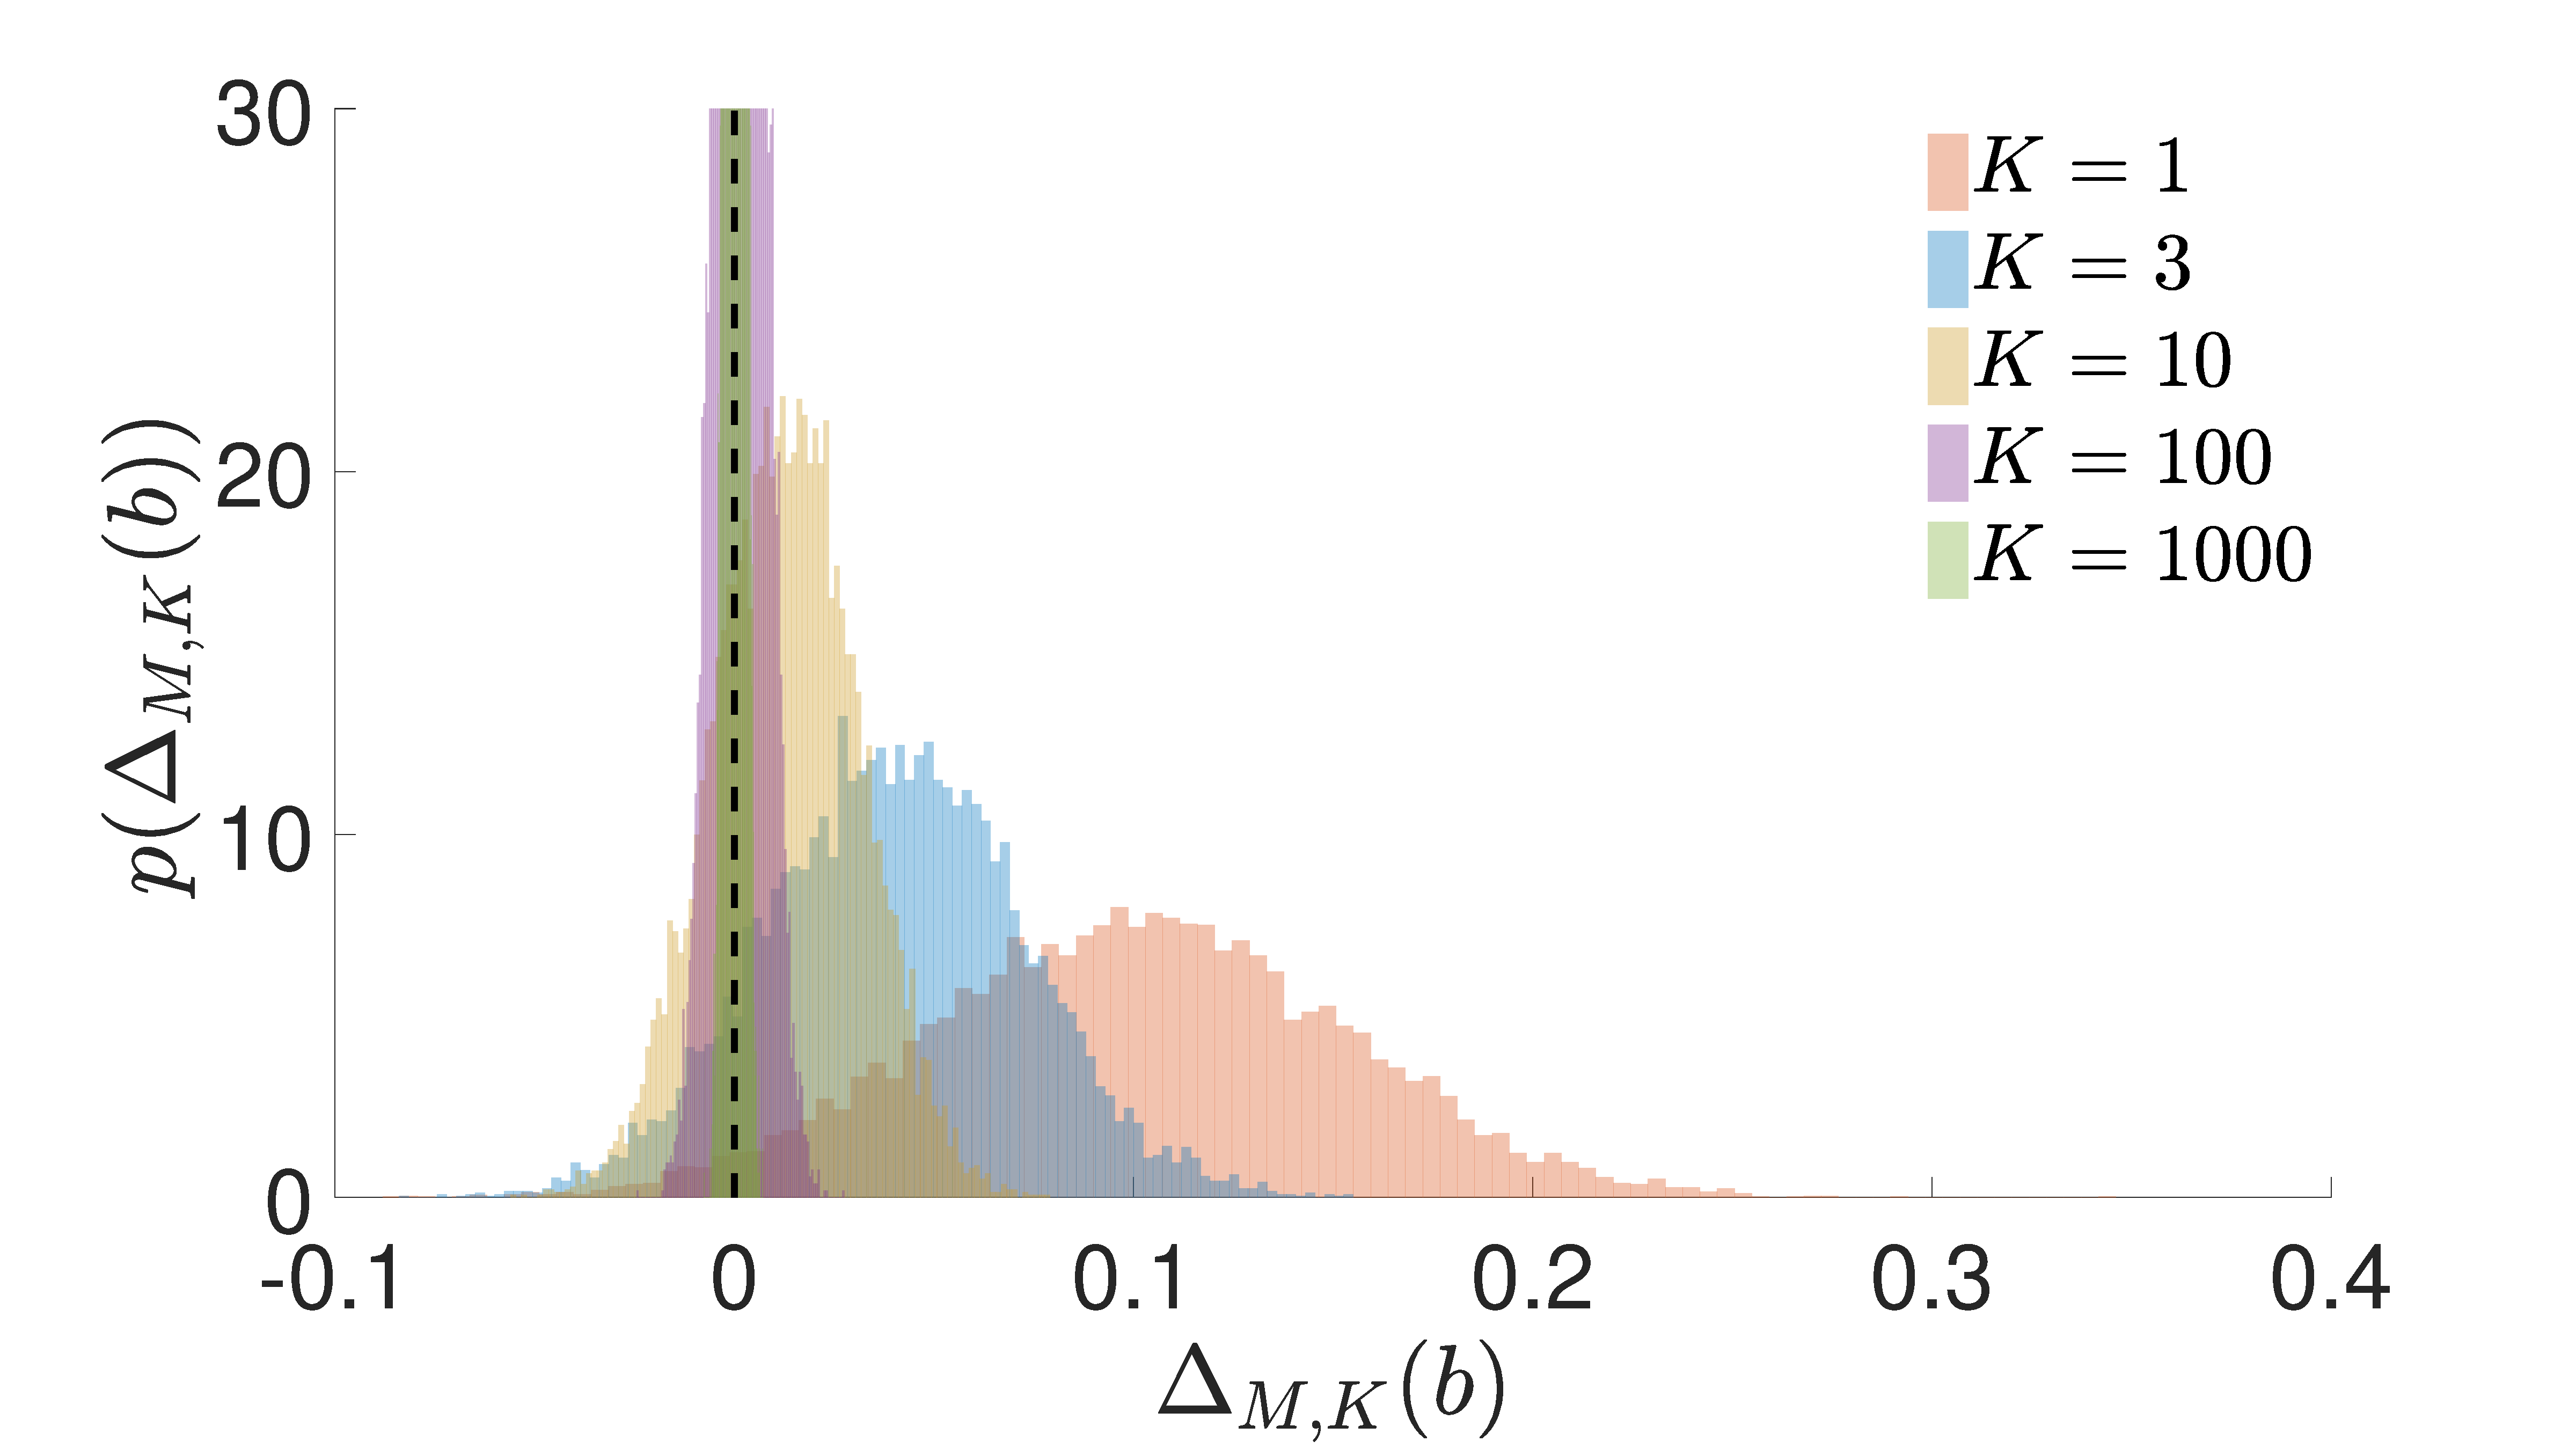
\includegraphics[width=\textwidth]{b_hist_IWAE} %\vspace{-2pt}
		\caption{ \gls{IWAE} inference network gradient estimates \label{fig:snr/b_hist_iwae}}
	\end{subfigure} ~~~~~~~~~~~~~
	%	\begin{subfigure}[b]{0.49\textwidth}
	%		\centering
	%		\includegraphics[width=\textwidth]{b_hist_VAE}
	%		\caption{\gls{VAE} inference network gradient estimates \label{fig:snr/b_hist_vae}}
	%	\end{subfigure}\\
	\begin{subfigure}[b]{0.4\textwidth}
		\centering
		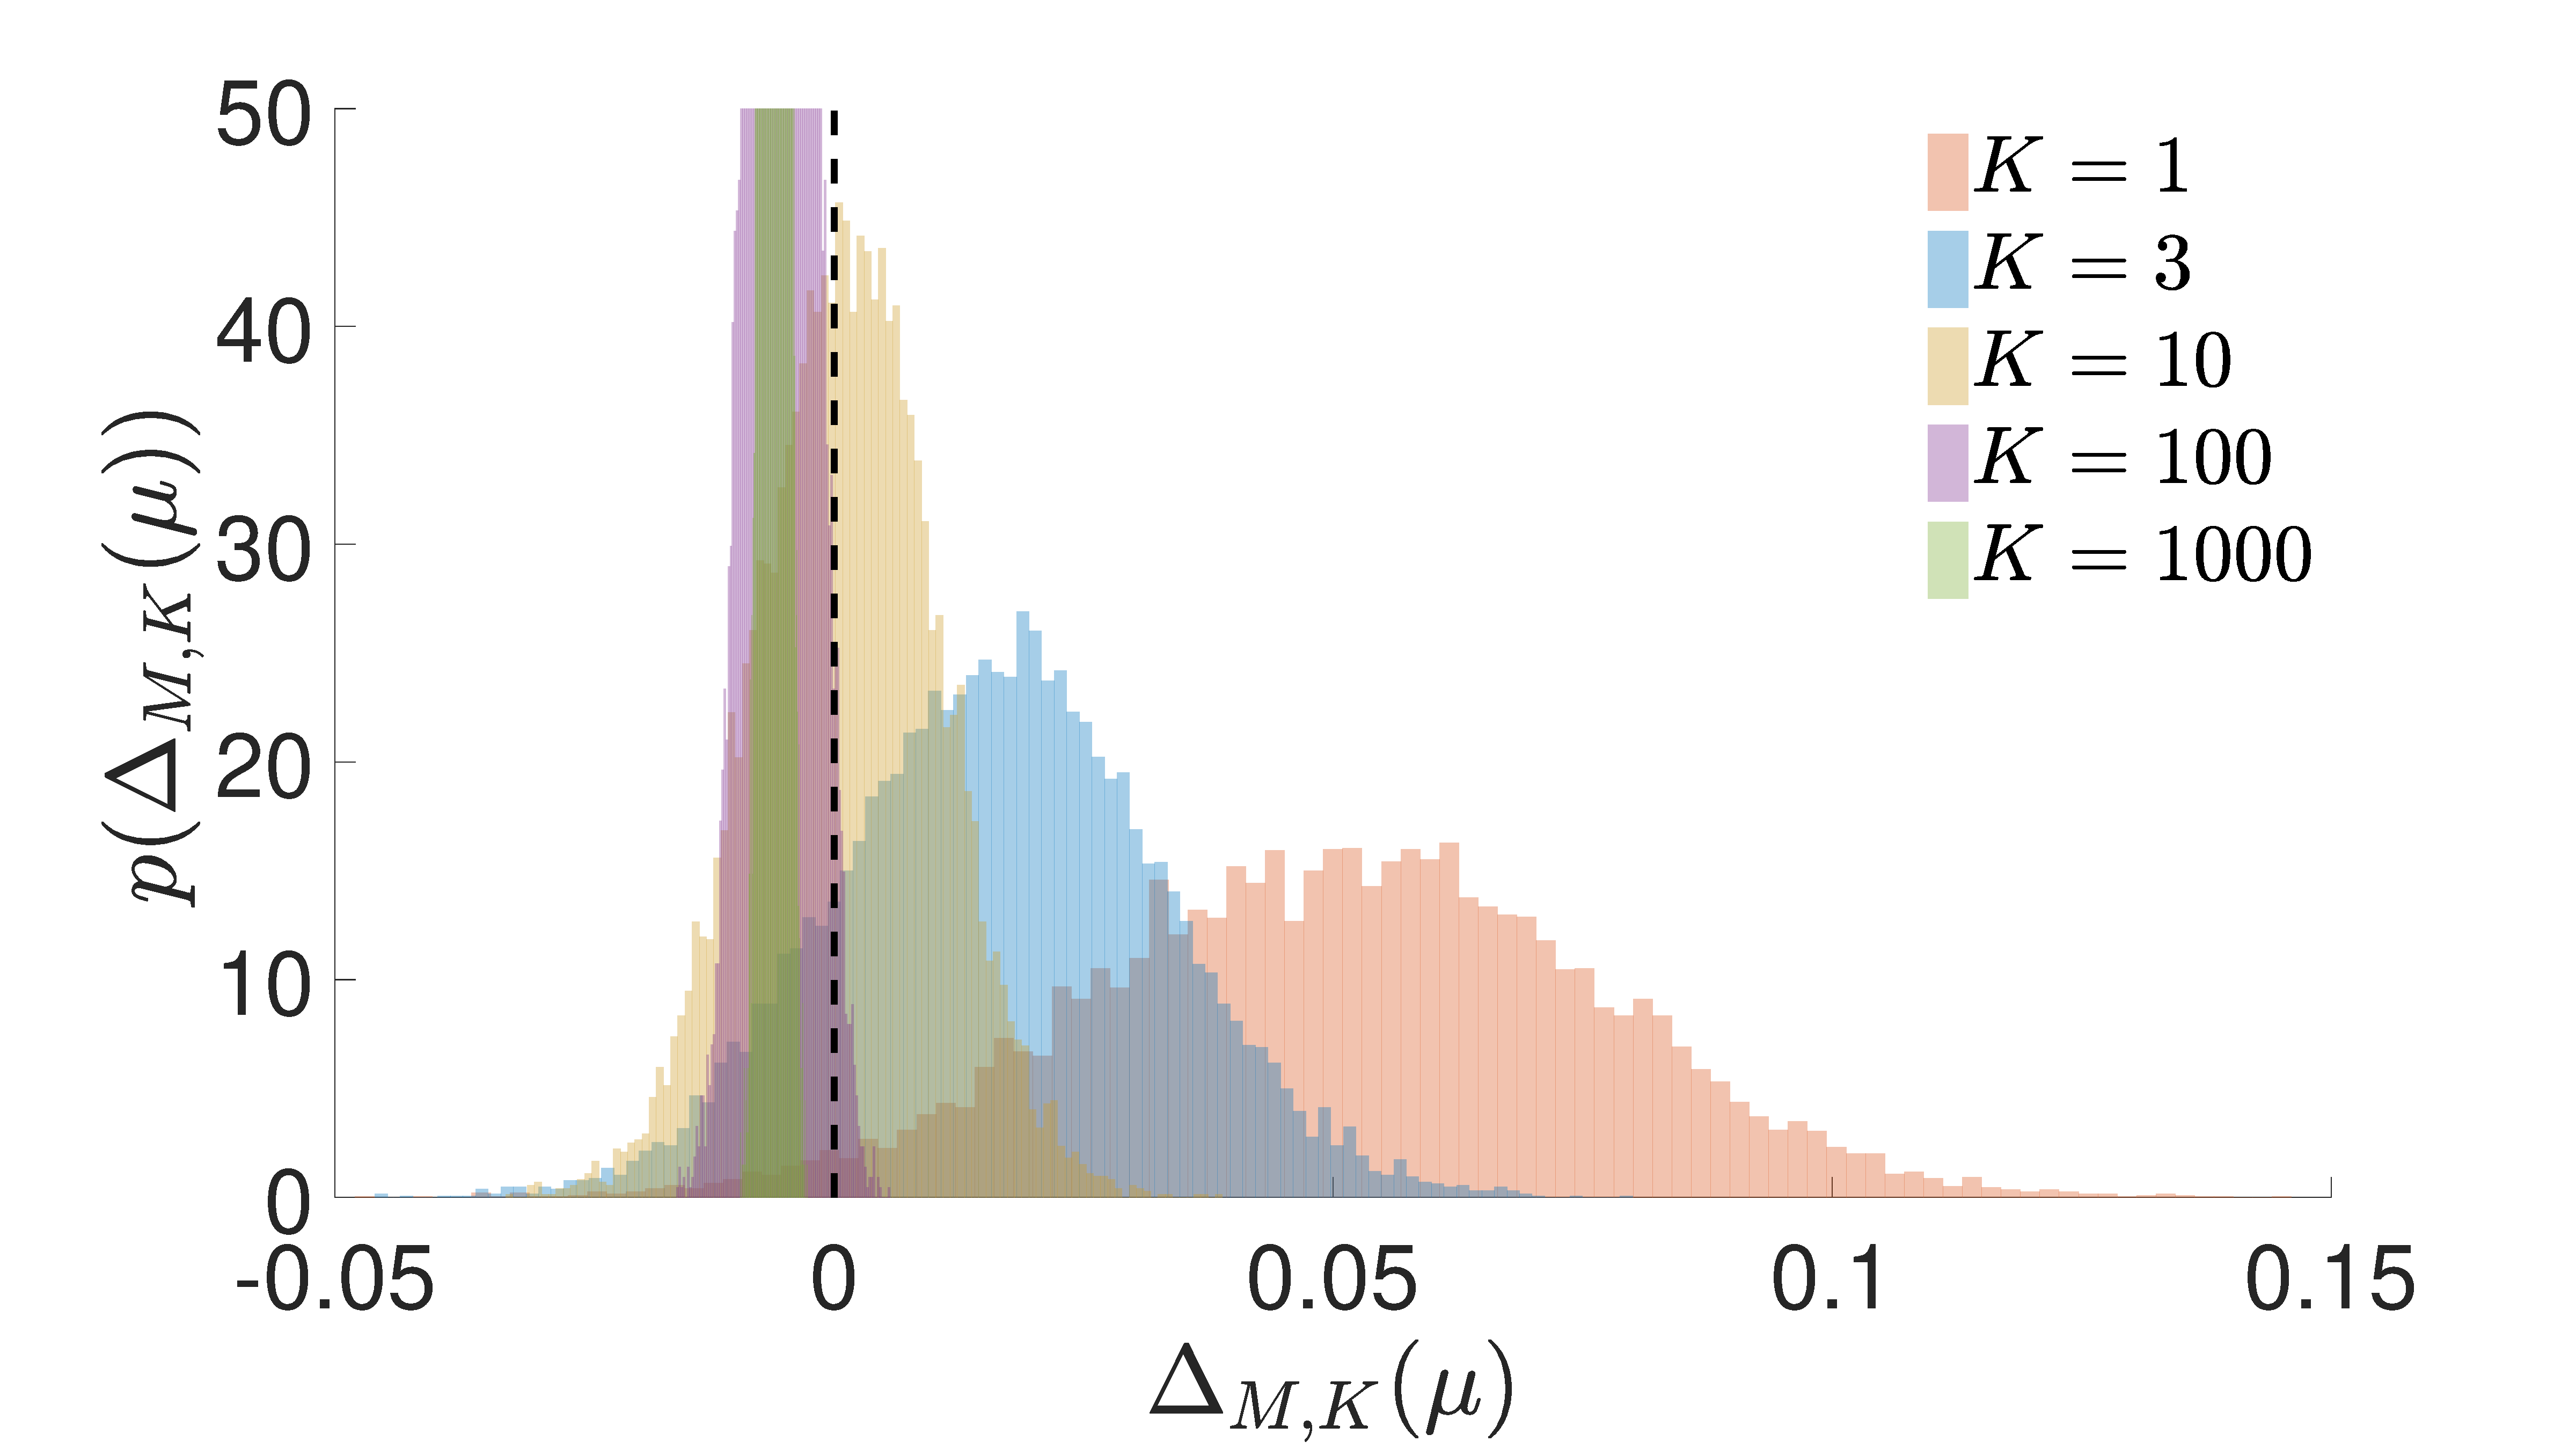
\includegraphics[width=\textwidth]{mu_hist_IWAE} %\vspace{-2pt}
		\caption{ \gls{IWAE} generative network gradient estimates \label{fig:snr/mu_hist_iwae}}
	\end{subfigure}\vspace{-6pt}
	%	\begin{subfigure}[b]{0.49\textwidth}
	%		\centering
	%		\includegraphics[width=\textwidth]{mu_hist_VAE}
	%		\caption{\gls{VAE} generative network gradient estimates \label{fig:snr/mu_hist_vae}}
	%	\end{subfigure}
	\caption{Histograms of gradient estimates $\Delta_{M,K}$ for the generative network and 
		the inference network using the \gls{IWAE} ($M=1$)
		objective with different values of $K$.
			\vspace{-14pt}
		\label{fig:snr/hists}}
\end{figure*}

\subsection{Multiple Data Points}
\label{sec:multi}

%Not only does this show that, for a given budget $T=MK$, then
%it is (at least asymptotically) better to increase $M$ instead of $K$
% to improve $\SNR_{M,K} (\phi)$, but also that
%increasing our overall budget for a fixed $M$ actually diminishes $\SNR_{M,K} (\phi)$.

	Typically when training deep generative models, one does not optimize a single \gls{ELBO}
	but instead its average over multiple data points, i.e.
	\begin{align}
	\label{eq:J}
	\mathcal J(\theta, \phi) &:= 
	\frac{1}{N} \sum\nolimits_{n = 1}^N \ELBO_{\text{IS}} (\theta, \phi, x^{(n)}).
	\end{align}
	Our results extend to this setting because the $z$ are drawn independently for each $x^{(n)}$, so
	\begin{align}
	\hspace{-4pt}\E\left[\frac{1}{N} \sum\nolimits_{n=1}^{N} \Delta_{M,K}^{(n)}\right]\hspace{-2pt} &=\hspace{-2pt}\frac{1}{N}\sum\nolimits_{n=1}^{N}
	\E\left[\Delta_{M,K}^{(n)}\right], \displaybreak[0] \\
	\hspace{-4pt}\text{Var}\left[\frac{1}{N} \sum\nolimits_{n=1}^{N} \Delta_{M,K}^{(n)}\right]\hspace{-2pt} &=\hspace{-2pt}\frac{1}{N^2}\sum\nolimits_{n=1}^{N}
	\text{Var}\left[\Delta_{M,K}^{(n)}\right]\hspace{-2pt}.
	\end{align}
	We thus also see that if we are using mini-batches such that $N$ is a chosen parameter and the $x^{(n)}$ are
	drawn from the empirical data distribution, then 
	the \glspl{SNR} of $\bar{\Delta}_{N,M,K} := \frac{1}{N} \sum_{n=1}^{N} \Delta_{M,K}^{(n)}$ scales as $\sqrt{N}$, i.e.
$\SNR_{N,M,K} (\theta) = O(\sqrt{NMK})$ and $\SNR_{N,M,K} (\phi) 
= O(\sqrt{NM/K})$.  Therefore increasing $N$ has the same ubiquitous benefit as increasing $M$.
In the rest of the paper, we will implicitly be considering the \glspl{SNR} for $\bar{\Delta}_{N,M,K}$, but
will omit the dependency on $N$ to simplify the notation.

% \begin{wrapfigure}{r}{0.24\textwidth}
% 	\centering
% 	\vspace{-10pt}
% 	\includegraphics[width=0.24\textwidth,trim={0 0 0 0.7cm},clip]{figures/gaussian_gradient.pdf}
% 	\vspace{-20pt}
% 	\caption{Density estimate of $\nabla_{\phi} \ELBO$
% 		for different $K$ \label{fig:kde}}
% 	\vspace{-12pt}
% \end{wrapfigure}
% %At a high-level, our argument that increasing $K$ can be detrimental to 
% %training the inference network is that even though
% %$\sigma[\nabla_{\phi} \log \hat{Z}_K]$ reduces as $K$ increases, 
% %$\nabla_{\phi} \ELBO$ also decreases because
% %more accurate estimates for $\hat{Z}_K$ can be achieved
% %for a wide range of proposal parameters $\phi$ such that the impact of $\phi$
% %diminishes.
% %Furthermore, as $\nabla_{\phi} \ELBO$
% %decreases faster than $\sigma[\nabla_{\phi} \log \hat{Z}_K]$, $\SNR_{\phi}(K)$
% %decreases as $K$ increases.
% %Typically, this shrinkage happens faster than
% %increasing $K$ reduces the standard deviation of the estimate and so the 
% %\gls{SNR} for inference network actually decreases, even though
% %it is a lower variance estimate.  
% The effect suggested by our previous theoretical result
% is demonstrated in Figure~\ref{fig:kde},
% showing a kernel density estimator for the distribution of the \gls{ELBO} gradient
% estimate for different $K$ and a simple Gaussian unknown mean model.  
% We see that as we increase $K$, both the expected gradient estimate
% and its standard deviation decrease with $K$, but the former decreases faster
% such that $\SNR_{\phi}(K)$ decreases.
% This is perhaps easiest
% to appreciate by noting that for $K\ge10$, there is a roughly equal probability
% of the estimate being positive or negative, such that we are equally likely to increase or decrease
% the parameter value at the next \gls{SGA} iteration, inevitably leading to poor performance.
% On the other hand, when $K=1$, it is far more likely that the gradient estimate is positive
% than negative, and so there is clear drift to the gradient steps.  
% Note that using a larger
% $K$ should always give better performance at test time -- the implication of our
% result is that it may be better to learn $\phi$ using a smaller $K$. 


%
%
%It is already well established that increasing $K$ in the \gls{IWAE} leads to a tighter
%\gls{ELBO} and that choosing $K>1$ tends to lead to better 
%performance in learning the generative network~\citep{burda2016importance}.  Our
%assertion is that these improvements do not necessarily translate
%to improved gradient estimators or, by proxy, better \gls{SGA} schemes for
%the inference network.  Though, as we showed in the last section, 
%the global optimum for $\{\theta,\phi\}$ is independent of $K$, 
%changing $K$ can  significantly impact
%the variance and expected magnitude of the gradients.  
%

%
%
%More formally, we have ...
%
%We can further demonstrate our result using an informal theoretical
%argument.
%Our gradient estimate for the $K$ particle \gls{IWAE} is
%\begin{align}
%\label{eq:iwae}
%I_{K} = \nabla_{\phi} \log \left(\frac{1}{K} \sum_{k=1}^{K} \frac{p_{\theta}(x^k, y)}{q_{\phi}(x^k \given y)} \right),
%\end{align}
%where $I = \lim\limits_{K \rightarrow \infty} I_{K} = 0$ because
%with infinite samples, the estimate is exact and thus independent
%of the proposal parameters.  Now adapting the \gls{IWAE} result
%of~\citet{rainforth2017opportunities} shows that
%\begin{align}
%\label{eq:mse-bound}
%\E \left[I_{K}^2\right] = \E \left[\left(I_{K}-I\right)^2\right] \le \frac{C_0 ^2 \varsigma_1^4}{4 K^2}+\frac{C_0 ^2 \varsigma_1^4}{4 K^2}
%+\frac{\kappa_0^2 \varsigma_1^2}{K}+\frac{C_0 \kappa_0 \varsigma_1^3}{K^{3/2}}+O\left(\frac{1}{K^3}\right),
%\end{align}
%where $C_0$, $\kappa_0$ ($K_0$ in~\citet{rainforth2017opportunities}), 
%and $\varsigma_1$ are constants and we have set $N=1$ in their formulation.  
%Here the first $\frac{C_0 ^2 \varsigma_1^4}{4 K^2}$ and $O\left(\frac{1}{K^3}\right)$
%are ``bias terms'', i.e. $\left(\E \left[I_{K}\right]\right)^2 = \left(\nabla_{\phi} \ELBO\right)^2$, and
%the rest are variance terms.  We can now define our \gls{SNR} as follows
%\begin{align}
%\SNR = \frac{\nabla_{\phi} \ELBO}{\sqrt{\mathrm{Var}[I_{K}]}}
%\approx \sqrt{\frac{\frac{C_0 ^2 \varsigma_1^4}{4 K^2}+O\left(\frac{1}{K^3}\right)}
%	{\frac{C_0 ^2 \varsigma_1^4}{4 K^2}
%		+\frac{\kappa_0^2 \varsigma_1^2}{K}+\frac{C_0 \kappa_0 \varsigma_1^3}{K^{3/2}}}}
%\approx \sqrt{\frac{C_0 ^2 \varsigma_1^2}{4 \kappa_0^2 K}} =
%O\left(\sqrt{\frac{1}{K}}\right),
%\end{align}
%where we have substituted in the bounds for the bias and variance
%from~\eqref{eq:mse-bound} and the approximations will, in general, become increasingly
%exact as $K$ increases.  We thus see that increasing $K$ reduces the \gls{SNR} and
%so a lower $K$ is preferable for training the inference network.  Alternatively
%we can think of this in terms of the standard deviation of our estimate increasing
%as $O(\sqrt{K})$ relative to the true gradient.
%


% !tex root=./main.tex

\vspace*{-1ex}
\section{EXPERIMENTS}
\vspace*{-1ex}
\label{sec:experiments}

% Purpose of experiments
% - run rws and iwae on something else than MNIST
% - compare rws to all other methods
% - confirm tighter is not necessarily better and effect on generative model
% - gradient estimator of ww is lower variance than that of iwae
% - mode collapse of ww, check if defensive rws helps
% - badness of ws
% - revisiting competitiveness of rws on large models
% - check whether claims hold for continuous

The \gls{IWAE} and \gls{RWS} algorithms have primarily been applied to problems with continuous latent variables and/or discrete latent variables that do not actually induce branching (such as sigmoid belief networks;~\cite{neal1992connectionist}).
%
The purpose of the following experiments is to compare \gls{RWS} to \gls{IWAE} combined with control variates and continuous relaxations (c.f \cref{sec:method}) on models with conditional branching, and show that it outperform such methods.
%
We empirically demonstrate that increasing the number of particles $K$ can be detrimental in \gls{IWAE} but advantageous in \gls{RWS}, as evidenced by achieved \glspl{ELBO} and average distance between true and amortized posteriors.
% \begin{compactitem}
%   \item , \label{experiment-point-1}
%   \item \gls{RWS} has a lower variance gradient estimator for $\phi$ than \gls{IWAE}, and
% \end{compactitem}
%

In the first experiment, we present learning and amortized inference in a \gls{PCFG}~\citep{booth1973applying}, an example \gls{SCFM} where continuous relaxations are inapplicable.
We demonstrate that \gls{RWS} outperforms \gls{IWAE} with a control variate both in terms of learning and inference.
The second experiment focuses on \glsreset{AIR}\gls{AIR}, the deep generative model of \cite{eslami2016attend}.
It demonstrates that \gls{RWS} leads to better learning of the generative model in a setting with both discrete and continuous latent variables, for modeling a complex visual data domain (c.f. \cref{sec:experiments/air}).
The final experiment involves a \gls{GMM} (\cref{sec:experiments/gmm}), thereby serving as a pedagogical example.
It explains the causes of why \gls{RWS} might be preferable to other methods in more detail.
\footnote{In \cref{app:sigmoid_belief_nets}, we include additional experiments on sigmoid belief networks which, however, are not \glspl{SCFM}.}

% The first experiment (\cref{sec:experiments/gmm}) aims to address all three points in a simple \gls{GMM} with a discrete latent variable used to select cluster locations.
% The next experiment, on \gls{AIR} (\cref{sec:experiments/air}), addresses the first point in a model containing both discrete latent variables used for branching as well as continuous latent variables in a more complex visual data domain.
% Finally, the \acrshort{MNIST} experiment (\cref{sec:experiments/mnist}) addresses the first point in a model with continuous latent variables.
%

% \todo{Didn't move this block to before ``Advantages of Reweighted Wake-Sleep'' because defensive \gls{RWS} is not introduced by then yet}
Notationally, the different variants of \gls{RWS} will be referred to as \gls{WS} and \gls{WW}.
The \emph{wake-phase $\theta$ update} is always used.
We refer to using it in conjunction with the \emph{sleep-phase $\phi$ update} as \acrshort{WS} and using it in conjunction with the \emph{wake-phase $\phi$ update} as \acrshort{WW}.
% %
% The variants differ in
% \begin{tabular}{@{}>{\bfseries}r@{\,\,}p{80ex}@{}}
%   \acrshort{WS} --  & using the \emph{sleep-phase $\phi$ update}, \\
%   \acrshort{WW} --  & using the \emph{wake-phase $\phi$ update}.
%   % \gls{WWS} -- & using both wake and sleep gradient estimators of $\phi$ where the
%   % gradient estimator is a uniform mixture of the two separate estimators.
% \end{tabular}
% %
Using both \emph{wake-} and \emph{sleep-phase $\phi$ updates} doubles the required stochastic sampling while yielding only minor improvements on the models we considered.
%
The number of particles $K$ used for the \emph{wake-phase $\theta$} and \emph{$\phi$ updates} is always specified, and computation between them is matched so
a \emph{wake-phase $\phi$ update} with batch size $B$ implies a \emph{sleep phase $\phi$ update} with $KB$ samples.

\subsection{PROBABILISTIC CONTEXT-FREE GRAMMAR}
\label{sec:experiments/pcfg}

% \begin{figure}
%   \includegraphics[width=\linewidth]{figures/pcfg/errors_end_points.pdf}
%   \caption{}
%   \label{fig:experiments/pcfg/astronomers_errors}
% \end{figure}
\begin{figure*}
  \centering
  % \includegraphics[width=0.94\textwidth]{figures/pcfg/errors.pdf}
  \includegraphics[width=\textwidth]{figures/pcfg/errors_vector.pdf}
  \vspace*{-0.7\baselineskip}
  \caption{
    \Gls{PCFG} training.
    \emph{(Top)}
    Quality of the generative model:
    While all methods have the same gradient update for $\theta$, the performance of \gls{WS} improves and is the best as $K$ is increased.
    Other methods, including \gls{WW}, do not yield significantly better model learning as $K$ is increased, since \gls{WS}'s inference network learns the fastest.
    \emph{(Bottom)}
    Quality of the inference network:
    \Gls{VIMCO} and \acrshort{REINFORCE} do not improve with increasing $K$.
    \Gls{WS} performs best as $K$ is increased, and while \gls{WW}'s performance improves, the improvement is not as significant.
    This can be attributed to the data-distribution bias being less significant than the bias coming from self-normalized \gls{IS} (c.f. \cref{sec:disadvantages}).
    Median and interquartile ranges from up to $10$ repeats shown (see text).
  }
  \label{fig:experiments/pcfg/astronomers_errors}
  \vspace*{-2ex}
\end{figure*}

% \begin{figure*}
%   \includegraphics[width=\textwidth]{figures/pcfg/both_errors.pdf}
%   \caption{}
%   \label{fig:experiments/pcfg/astronomers_errors}
% \end{figure*}

In this experiment we learn model parameters and amortize inference in a \gls{PCFG}~\citep{booth1973applying}.
Each discrete latent variable in a \gls{PCFG} chooses a particular child of a node in a tree.
Depending on each discrete choice, the generative model can lead to different future latent variables.
A \gls{PCFG} is an example of an \gls{SCFM} where continuous relaxations cannot be applied---weighing combinatorially many futures by a continuous relaxation is infeasible and doing so for futures which have infinite latent variables is impossible.

While supervised approaches have recently led to state-of-the-art performance in parsing~\citep{chen2014fast}, \glspl{PCFG} remain one of the key models for unsupervised parsing~\citep{manning1999foundations}.
Learning in a \gls{PCFG} is typically done via expectation-maximization~\citep{dempster1977maximum} which uses the inside-outside algorithm~\citep{lari1990estimation}.
Inference methods are based on dynamic programming~\citep{younger1967recognition,earley1970efficient} or search~\citep{klein2003parsing}.
Applying \gls{RWS} and \gls{IWAE} algorithms to \glspl{PCFG} allows learning from large unlabeled datasets through \gls{SGD} while inference amortization ensures linear-time parsing in the number of words in a sentence, at test-time.
Moreover, using the inference network as a proposal distribution in \gls{IS} provides asymptotically exact posteriors if parses are ambiguous.

% generative model
A \gls{PCFG} is defined by sets of terminals (or words) $\{t_i\}$, non-terminals $\{n_i\}$, production rules $\{n_i \to \zeta_j\}$ with $\zeta_j$ a sequence of terminals and non-terminals, probabilities for each production rule such that $\sum_j~P\left(n_i \!\to\! \zeta_j\right)~=~1$ for each $n_i$, and a start symbol $n_1$.
% A \gls{PCFG} is defined by a set of terminals (or words) $\{t_i\}$, a set of non-terminals $\{n_i\}$, a start symbol $n_1$, a set of production rules $\{n_i \to \zeta_j\}$, with $\zeta_j$ a sequence of terminals and non-terminals, and a set of probabilities for each production rule such that $\sum_j~P\left(n_i \to \zeta_j\right)~=~1$ for each $n_i$.
Consider the \emph{Astronomers \gls{PCFG}} given in \citet[Table
11.2]{manning1999foundations} (c.f. \cref{app:pcfg}).
A parse tree $z$ is obtained by recursively applying the production rules until there are no more non-terminals.
For example, a parse tree (S (NP astronomers) (VP (V saw) (NP stars))) is obtained by applying the production rules as follows:

\par\nobreak\vspace{-1.2em}
{\small
\begin{align*}
  \text{S} \xrightarrow{1.0} \text{NP}\,\text{VP} \xrightarrow{0.1} \text{astronomers}\,\text{VP} \xrightarrow{0.7} \text{astronomers}\,\text{V}\,\text{NP} \\
  \,\xrightarrow{1.0} \text{astronomers}\,\text{saw}\,\text{NP} \xrightarrow{0.18} \text{astronomers}\,\text{saw}\,\text{stars},
\end{align*}
}%
where the probability $p(z)$ is obtained by multiplying the corresponding production probabilities as indicated on top of the arrows.
The likelihood of a \gls{PCFG}, $p(x \given z)$, is $1$ if the sentence $x$ matches the sentence produced by $z$ (in this case ``astronomers saw stars'') and $0$ otherwise.
One can easily construct infinitely long $z$ by choosing productions which contain non-terminals, for example: $\text{S} \to \text{NP}\,\text{VP} \to \text{NP}\,\text{PP}\,\text{VP} \to \text{NP}\,\text{PP}\,\text{PP}\,\text{VP} \to \cdots$.

% Grammars let us identify structure in sentences.
% In many situations, the underlying structure of a sentence is ambiguous.
% Take, for instance the sentence ``astronomers saw stars with telescopes.''
% This sentence could be interpreted either as i) the astronomers used telescopes to see stars or ii) the astronomers saw stars which had telescopes.
% % what are pcfgs?
% \Glspl{PCFG}~\citep{manning1999foundations} allow us to handle such ambiguities by modeling the joint distribution over the structure $z$, which is represented as a parse tree, and the sentence $x$.

% p, q architecture
We learn the production probabilities of the \gls{PCFG} and an inference network computing the conditional distribution of a parse tree given a sentence.
%
The architecture of the inference network is the same as described in \citep[Section 3.3]{le2017inference} except the input to the \gls{RNN} consists only of the sentence embedding, previous sample embedding, and an address embedding.
%
Each word is represented as a one-hot vector and the sentence embedding is obtained through another \gls{RNN}.
%
Instead of a hard $\{0, 1\}$ likelihood which can make learning difficult, we use a relaxation, $p(x \given z) = \exp(-L(x, s(z))^2)$, where $L$ is the Levenshtein distance and $s(z)$ is the sentence produced by $z$.
%
Using the Levenshtein distance can also be interpreted as an instance of approximate Bayesian computation~\citep{sisson2018handbook}.
%
Training sentences are obtained by sampling from the \emph{astronomers} \gls{PCFG} with the true production probabilities.
%, discarding the corresponding parse trees.

% why ws is better?
We run \gls{WW}, \gls{WS}, \gls{VIMCO} and \acrshort{REINFORCE} ten times for $K \in \{2, 5, 10, 20\}$, with batch size \(B=2\), using the Adam optimizer~\citep{kingma2015adam} with default hyperparameters.
%
We observe that the inference network can often end up sub-optimally sampling very long $z$ (by choosing production rules with many non-terminals), leading to slow and ineffective runs.
%
We therefore cap the run-time to $100$ hours---out of ten runs, \gls{WW}, \gls{WS}, \gls{VIMCO} and \acrshort{REINFORCE} retain on average $6$, $6$, $5.75$ and $4$ runs respectively
%
In \cref{fig:experiments/pcfg/astronomers_errors}, we show both
%
\begin{inparaenum}[(i)]
\item the quality of the generative model as measured by the average \gls{KL} between the true and the model production probabilities, and
\item the quality of the inference network as measured by $\E_{p(x)}[\KL(p(z \given x), q_\phi(z \given x))]$ which is estimated up to an additive constant (the conditional entropy $H(p(z \given x))$) by the sleep-$\phi$ loss \cref{eq:sleep-phi-obj} using samples from the true \gls{PCFG}.
\end{inparaenum}

Quantitatively, \gls{WS} improves as $K$ increases and outperforms \gls{IWAE}-based algorithms both in terms of learning and inference amortization.
While \gls{WW}'s inference amortization improves slightly as $K$ increases, it is significantly worse than \gls{WS}'s.
This is because \gls{IS} proposals will rarely produce a parse tree $z$ for which $s(z)$ matches $x$, leading to extremely biased estimates of the wake-$\phi$ update.
In this case, this bias is more significant than that of the data-distribution which can harm the sleep-$\phi$ update.

%
We inspect the quality of the inference network by sampling from it.
%
\Cref{fig:experiments/pcfg/ws_q_samples}, shows samples from an inference network trained with \gls{WS}, conditioned on the sentence ``astronomers saw stars with telescopes'', weighted according to the frequency of occurrence.
%
\Cref{app:pcfg} further includes samples from an inference network trained with \gls{VIMCO}, showing that none of them match the given sentence ($s(z) \neq x$), and whose production probabilities are poor, unlike with \gls{RWS}.

\begin{figure}[t]
  \centering
  % \vspace*{-1.5\baselineskip}
  \includegraphics[width=0.95\linewidth]{figures/pcfg/ws_q_samples.eps}
  \caption{
    Samples from the inference network trained with \gls{WS} ($K = 20$).
    %
    Highest probability samples correspond to correct sentences ($s(z) = x$).
  }
  \label{fig:experiments/pcfg/ws_q_samples}
  \vspace*{-2ex}
\end{figure}

% \begin{figure*}
%   \includegraphics[width=\textwidth]{figures/pcfg/ws.eps}
%   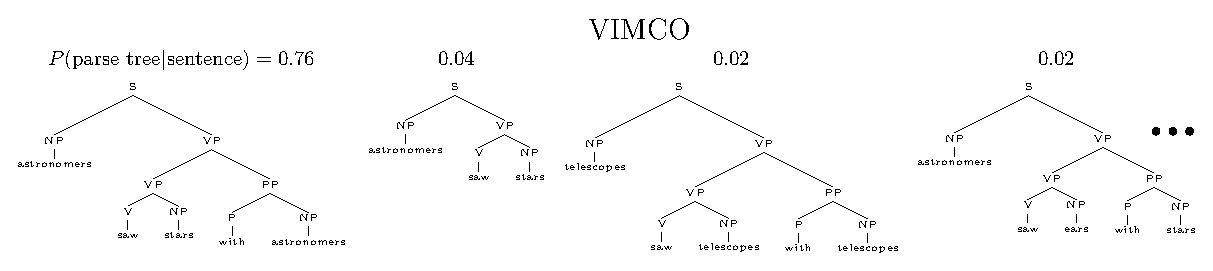
\includegraphics[width=\textwidth]{figures/pcfg/vimco.eps}
% \end{figure*}

% p(tree1 | sentence) = 0.42857142857
% p(tree2 | sentence) = 0.57142857142

\begin{figure*}[!ht]
  \includegraphics[width=0.33\textwidth]{figures/air/logp_test.pdf}
  \includegraphics[width=0.33\textwidth]{figures/air_logp_end_2.pdf}
  \includegraphics[width=0.33\textwidth]{figures/air/kl_test.pdf}
  \caption{
    Training of \gls{AIR}.
    \emph{(Left)}
    Training curves:
    % there is larger variance in models learned with \gls{VIMCO}.
    training with \gls{VIMCO} leads to larger variance in training than \gls{WW}.
    \emph{(Middle)}
    Log evidence values at the end of training:
    increasing number of particles improves \gls{WW} monotonically but improves \gls{VIMCO} only up to a point ($K = 10$ is the best).
    \emph{(Right)}
    \gls{WW} results in significantly lower variance and better inference networks than \gls{VIMCO}.
    Note that \gls{KL} is between the inference network and the \emph{current} generative model.
  }
  \label{fig:air_logp}
  \vspace*{-2ex}
\end{figure*}

\subsection{ATTEND, INFER, REPEAT}
\label{sec:experiments/air}

% model
Next, we evaluate \gls{WW} and \gls{VIMCO}
% (the best performing \gls{IWAE}-based algorithm for the \gls{GMM})
on \gls{AIR}~\citep{eslami2016attend}, a structured deep generative model with both discrete and continuous latent variables.
%
\Gls{AIR} uses the discrete variable to decide how many continuous variables are necessary to explain an image.
%
The sequential inference procedure of \gls{AIR} poses a difficult problem, since it implies a sequential decision process with possible branching.
%
See \citep{eslami2016attend} and \cref{app:air} for the model notation and details.

% training
We set the maximum number of inference steps in \gls{AIR} to three and train on $50 \times 50$ images with zero, one or two \acrshort{MNIST} digits.
%
The training and testing data sets consist of $60000$ and $10000$ images respectively, generated from the respective \acrshort{MNIST} train/test datasets.
%
Unlike \gls{AIR}, which used Gaussian likelihood with fixed standard deviation and continuous inputs (i.e., input $\mathbf{x} \in [0, 1]^{50 \times 50}$), we use a Bernoulli likelihood and binarized data; the stochastic binarization is similar to \citet{burda2016importance}.
%
% This choice is motivated by initial experiments, which have shown that the original setup is detrimental to the sleep phase of \gls{WS} -- samples from the generative model did not look similar to true data even after the training has converged.
%
Training is performed over two million iterations by RmsProp \citep{tieleman2012rms} with the learning rate of $10^{-5}$, which is divided by three after $400$k and $1000$k training iterations.
%
We set the glimpse size to $20 \times 20$.

% evaluation
We first evaluate the generative model via the average test log marginal where each log marginal is estimated by a one-sample, $5000$-particle \gls{IWAE} estimate.
%
The inference network is then evaluated via the average test \gls{KL} from the inference network to the posterior under the current model where each $\KL(q_\phi(z \given x), p_\theta(z \given x))$ is estimated as a difference between the log marginal estimate above and a $5000$-sample, one-particle \gls{IWAE} estimate.
%
Note that this estimate is just a proxy to the desired \gls{KL} from the inference network to the \emph{true} model posterior.
%
% Finally, we approximate the accuracy of number of inference steps as a proxy for the qualities of both the generative model and inference network.

% result
This experiment confirms that increasing number of particles improves \gls{VIMCO} only up to a point, whereas \gls{WW} improves monotonically with increased~\(K\) (\cref{fig:air_logp}).
%
\Gls{WW} also results in significantly lower variance and better inference networks than \gls{VIMCO}.

%%%%%%%%%%%%%%%%%%%%%%%%%%%%%%%%%%%%%%%%%%%%%%%%%%%%%%%%%%%%%%%%%%%%%%%%%%%%%%
% Run eval and restore !!!!!!!!!!!!!!!!!!!!!!!!!!!!!!!!!!
%
%
% the below num steps accuracy in AIR is importance-resampled, with different number of particles for every model (the same K as used for training); for this reason I don't think it is valid to report it as is. I think I can still evaluate it for M=100, say, and K=1 (k=1 to emphasise quality of q). For now, though, it's misleading.
%
%
%
%    \begin{table}[ht]
%      \centering
%      \caption{Accuracy of number of inference steps in \gls{AIR} is better for \gls{WW} than \gls{VIMCO}.}
%      \label{table:air_accuracy}
%      \begin{tabular}{@{}llllll@{}}
%      \toprule
%      $K$ & $5$ & $10$ & $20$ & $40$ & $80$ \\ \midrule
%      \gls{IWAE} & $0.949 \pm 0.063$ & $0.997 \pm 0.001$ & $0.997 \pm 0.000$ & $0.830 \pm 0.289$ & $0.997 \pm 0.002$ \\
%      \gls{WW}   & $0.997 \pm 0.000$ & $0.997 \pm 0.000$ & $0.997 \pm 0.000$ & $0.983 \pm 0.025$ & $0.996 \pm 0.001$ \\ \bottomrule
%      \end{tabular}
%    \end{table}
%%%%%%%%%%%%%%%%%%%%%%%%%%%%%%%%%%%%%%%%%%%%%%%%%%%%%%%%%%%%%%%%%%%%%%%%%%%

    % \begin{figure}
    %     \centering
    %     \includegraphics[width=0.5\linewidth]{air/logp_test}
    %     \caption{AIR: Marginal log likelihood. Solid lines are means and shaded regions represent one standard deviation. Standard deviation has been omitted for cases where the mean standard deviation is greater than $5$.}
    %     \label{fig:air_logp}
    % \end{figure}

    % \begin{figure}
    %     \centering
    %     \includegraphics[width=0.5\linewidth]{air/vae_test}
    %     \caption{AIR: The evidence lower-bound. Solid lines are means and shaded regions represent one standard deviation. Standard deviation has been omitted for cases where the mean standard deviation is greater than $5$.}
    %     \label{fig:air_vae}
    % \end{figure}

    % \begin{figure}
    %     \centering
    %     \includegraphics[width=0.5\linewidth]{air/kl_test}
    %     \caption{AIR: KL-divergence between the approximate posterior and the posterior of the current model. Solid lines are means and shaded regions represent one standard deviation. Standard deviation has been omitted for cases where the mean standard deviation is greater than $5$.}
    %     \label{fig:air_acc}
    % \end{figure}

    % \begin{figure}
    %     \centering
    %     \includegraphics[width=0.5\linewidth]{air/num_step_acc_test}
    %     \caption{AIR: Accuracy of number of inference steps. Solid lines are means and shaded regions represent one standard deviation. Standard deviation has been omitted for cases where the mean standard deviation is greater than $0.1$.}
    %     \label{fig:air_acc_2}
    % \end{figure}




%numbers for AIR:
%
%tag, target, k, mean+-std, mean_std_across_training
%
%vae_test
%vae_test, iwae_vimco, 80, -461.778+-194.494 214.07364
%vae_test, iwae_vimco, 40, -268.693+-234.041 196.0884
%vae_test, iwae_vimco, 20, -154.271+-43.617 19.922382
%vae_test, iwae_vimco, 10, -183.581+-80.310 38.15588
%vae_test, iwae_vimco, 5, -113.130+-9.452 7.988214
%vae_test, rw_rw, 80, -103.821+-0.086 0.27857488
%vae_test, rw_rw, 40, -104.072+-0.759 0.67278016
%vae_test, rw_rw, 20, -103.609+-0.265 0.32347438
%vae_test, rw_rw, 10, -104.129+-0.301 0.35700417
%vae_test, rw_rw, 5, -104.523+-0.252 0.3047606
%vae_test
%vae_test, iwae_vimco, 80, -461.778+-194.494 214.07364
%vae_test, iwae_vimco, 40, -268.693+-234.041 196.0884
%vae_test, iwae_vimco, 20, -154.271+-43.617 19.922382
%vae_test, iwae_vimco, 10, -183.581+-80.310 38.15588
%vae_test, iwae_vimco, 5, -113.130+-9.452 7.988214
%vae_test, rw_rw, 80, -103.821+-0.086 0.27857488
%vae_test, rw_rw, 40, -104.072+-0.759 0.67278016
%vae_test, rw_rw, 20, -103.609+-0.265 0.32347438
%vae_test, rw_rw, 10, -104.129+-0.301 0.35700417
%vae_test, rw_rw, 5, -104.523+-0.252 0.3047606
%kl_test
%kl_test, iwae_vimco, 80, 355.846+-194.526 214.1097
%kl_test, iwae_vimco, 40, 165.203+-234.058 196.11067
%kl_test, iwae_vimco, 20, 55.454+-43.618 19.963625
%kl_test, iwae_vimco, 10, 84.986+-80.311 38.194466
%kl_test, iwae_vimco, 5, 13.805+-9.457 8.035896
%kl_test, rw_rw, 80, 6.978+-0.098 0.28919804
%kl_test, rw_rw, 40, 6.818+-0.797 0.7250941
%kl_test, rw_rw, 20, 5.995+-0.267 0.32935238
%kl_test, rw_rw, 10, 5.858+-0.323 0.37547684
%kl_test, rw_rw, 5, 5.362+-0.333 0.3886485
%kl_test
%kl_test, iwae_vimco, 80, 355.846+-194.526 214.1097
%kl_test, iwae_vimco, 40, 165.203+-234.058 196.11067
%kl_test, iwae_vimco, 20, 55.454+-43.618 19.963625
%kl_test, iwae_vimco, 10, 84.986+-80.311 38.194466
%kl_test, iwae_vimco, 5, 13.805+-9.457 8.035896
%kl_test, rw_rw, 80, 6.978+-0.098 0.28919804
%kl_test, rw_rw, 40, 6.818+-0.797 0.7250941
%kl_test, rw_rw, 20, 5.995+-0.267 0.32935238
%kl_test, rw_rw, 10, 5.858+-0.323 0.37547684
%kl_test, rw_rw, 5, 5.362+-0.333 0.3886485
%logpx_test
%logpx_test, iwae_vimco, 80, -105.932+-3.512 3.614406
%logpx_test, iwae_vimco, 40, -103.490+-2.875 2.5203645
%logpx_test, iwae_vimco, 20, -98.817+-0.268 0.75712645
%logpx_test, iwae_vimco, 10, -98.595+-0.378 0.7549159
%logpx_test, iwae_vimco, 5, -99.324+-0.283 0.42569834
%logpx_test, rw_rw, 80, -96.842+-0.046 0.0680763
%logpx_test, rw_rw, 40, -97.254+-0.243 0.2675206
%logpx_test, rw_rw, 20, -97.614+-0.033 0.051102422
%logpx_test, rw_rw, 10, -98.271+-0.116 0.10897209
%logpx_test, rw_rw, 5, -99.161+-0.218 0.23595817
%
%num_steps_acc_test, iwae_vimco, 80, 0.997+-0.002 0.0097846912577274
%num_steps_acc_test, iwae_vimco, 40, 0.830+-0.289 0.24703451530470122
%num_steps_acc_test, iwae_vimco, 20, 0.997+-0.000 0.005596457855210997
%num_steps_acc_test, iwae_vimco, 10, 0.997+-0.001 0.008849094343651977
%num_steps_acc_test, iwae_vimco, 5, 0.949+-0.063 0.06692072584329027
%num_steps_acc_test, rw_rw, 80, 0.996+-0.001 0.0008066281251088672
%num_steps_acc_test, rw_rw, 40, 0.983+-0.025 0.02411366072534301
%num_steps_acc_test, rw_rw, 20, 0.997+-0.000 0.00047535752918038856
%num_steps_acc_test, rw_rw, 10, 0.997+-0.000 0.0005349459234959429
%num_steps_acc_test, rw_rw, 5, 0.997+-0.000 0.000862527605328427

% \begin{figure}
%     \centering
%     \includegraphics[width=0.5\linewidth]{air/fixed_prior_iwae_test}
%     \caption{AIR with fixed priors: \textsc{IWAE}-5 bound. \ak{This is just to show correctness of IWAE+VIMCO implementation and should be moved into appendix in case of space issues.}}
%     \label{fig:air_iwae_fixed_prior}
% \end{figure}

% \begin{figure}
%     \centering
%     \includegraphics[width=0.5\linewidth]{air/fixed_prior_vae_test}
%     \caption{AIR with fixed priors: \textsc{IWAE}-5 bound. \ak{This is just to show correctness of IWAE+VIMCO implementation and should be moved into appendix in case of space issues.}}
%     \label{fig:air_iwae_fixed_prior_2}
% \end{figure}

\subsection{GAUSSIAN MIXTURE MODEL}
\label{sec:experiments/gmm}

\begin{figure*}[!ht]
  \centering
  % \includegraphics[width=0.9\textwidth]{figures/gmm/plot_paper.pdf}
  % \includegraphics[width=0.89\textwidth]{figures/gmm/errors.pdf}
  \includegraphics[width=\textwidth]{figures/gmm/errors_no_std.pdf}
  \vspace*{-4ex}
  \caption{
    \Gls{GMM} training.
    Median and interquartile ranges from $10$ repeats shown.
    \emph{(Top)}
    Quality of the generative model:
    \gls{WS} and \gls{WW} improve with more particles thanks to lower variance and lower bias estimators of the gradient respectively.
    \Gls{IWAE} methods suffer with a larger particle budget~\citep{rainforth2018tighter}.
    \Gls{WS} performs the worst as a consequence of computing the expected \gls{KL} under the model distribution~\(p_\theta(x)\)~\cref{eq:sleep-phi-obj} instead of the true data distribution~\(p(x)\) as with \gls{WW}~\cref{eq:wake-phi-obj}.
    \Gls{WW} suffers from branch-pruning (see text) in low-particle regimes, but learns the best model fastest in the many-particle regime; $\delta$-\gls{WW} additionally learns well in the low-particle regime.
    \emph{(Bottom)}
    Both inference network and generative model quality develop identically.
    % \emph{(Bottom)}
    % \Gls{WW} and \gls{WS} have lower-variance gradient estimators of $\phi$ than \gls{IWAE}, as they avoid the high-variance term \circled{1} in \eqref{eq:iwae-reinforce}.
    % This is a necessary, but not sufficient, condition for efficient learning, with other factors being gradient direction and the ability to escape local optima.
  }
  \label{fig:gmm}
  \vspace*{-1ex}
\end{figure*}

% model
% \setlength{\columnsep}{1pt}
% \begin{wrapfigure}[7]{r}{0.21\textwidth}
%   \centering
%   \vspace*{-3ex}
%   \includegraphics[width=0.95\linewidth,trim={1em 0 1em 1em},clip]{figures/gmm_true_dist.pdf}
%   \vspace*{-2.5ex}
%   \caption{True \gls{GMM}.}
%   \label{fig:true-gmm}
% \end{wrapfigure}
%
In order to examine the differences between \gls{RWS} and \gls{IWAE} more closely, we study  a \gls{GMM} which branches on a discrete latent variable to select cluster assignments.
The generative model and inference network are defined as
%
% {\footnotesize
\begin{align*}
  p_\theta(z) &= \mathrm{Cat}(z \given \mathrm{softmax}(\theta)),\,\,
  p(x \given z) = \mathcal{N}(x \given \mu_z, \sigma_z^2), \\
  q_\phi(z \given x) &= \mathrm{Cat}(z \given \mathrm{softmax}(\eta_\phi(x))),
\end{align*}
% }
%
where $z \in \{0, \dotsc, C - 1\}$,  $C$ is the number of clusters and $\mu_c, \sigma_c^2$ are fixed to $\mu_c = 10c$ and $\sigma_c^2 = 5^2$.
The generative model parameters are $\theta \in \mathbb R^C$.
The inference network consists of a \acrlong{MLP} $\eta_\phi: \mathbb R \to \mathbb R^C$, with the $1$-$16$-$C$ architecture and the $\tanh$ nonlinearity, parameterized by $\phi$.
The chosen family of inference networks is empirically expressive enough to capture the posterior under the true model.
The true model is set to $p_{\theta_\text{true}}(x)$ where $\mathrm{softmax}(\theta_\text{true})_c = (c + 5) / \sum_{i = 1}^C (i + 5)$ ($c = 0, \dotsc, C - 1$), i.e. the mixture probabilities are linearly increasing with the $z$
.
% (\cref{fig:true-gmm}).
We fix the mixture parameters in order to study the important features of the problem at hand in isolation.

% training details
We train using \gls{WS}, \gls{WW}, as well as using \gls{IWAE} with \acrshort{REINFORCE}, \acrshort{RELAX}, \gls{VIMCO} and the Concrete distribution.
%
We attempted different variants of relaxations \citep{rolfe2016dvae,vahdat2018dvaepp} in this setting, but they performed considerably worse than any of the alternatives (c.f. \Cref{app:dvae}).
%
We fix $C = 20$ and increase number of particles from $K = 2$ to $20$.
%
We use the Adam optimizer with default parameters.
%
Each training iteration samples a batch of $100$ data points from the true model.
%
Having searched over several temperature schedules for the Concrete distribution, we use the one with the lowest trainable terminal temperature (linearly annealing from $3$ to $0.5$).
%
We found that using the control variate $c_\rho(g_{1:K}) = \frac{1}{K} \sum_{k = 1}^K \acrshort{MLP}_\rho([x, g_k])$, with \gls{MLP} architecture $(1 + C)$-$16$-$16$-$1$ ($\tanh$) led to most stable training (c.f.\ \cref{app:gmm}).

% evaluation details
% We evaluate the generative model, inference network.
The generative model is evaluated via the $L_2$ distance between the \glspl{PMF} of its prior and true prior as $\|\mathrm{softmax}(\theta) - \mathrm{softmax}(\theta_\text{true})\|$.
The inference network is evaluated via the $L_2$ distance between \glspl{PMF} of the current and true posteriors, averaged over a fixed set~(\(M=100\)) of observations $(x_{\text{test}}^{(m)})_{m = 1}^{M}$ from the true model: $\frac{1}{M} \sum_{m = 1}^M \|q_\phi(z \given x_{\text{test}}^{(m)}) - p_{\theta_{\text{true}}}(z \given x_{\text{test}}^{(m)})\|$.
% Finally, \(\phi\)'s gradient-estimator standard deviation is given by $\frac{1}{D_\phi} \sum_{d = 1}^{D_\phi} \std(g_d)$ where $g_d$ is the $d$th (out of $D_\phi$) element of one of~\(\phi\)'s gradient estimators (e.g. \cref{eq:iwae-reinforce} for \acrshort{REINFORCE}) and $\std(\cdot)$ is estimated using $10$ samples.

% results & zero forcing & defensive IS
% Here, we demonstrate that increasing number of particles leads to better inference networks for \gls{WS} and \gls{WW} but not for \gls{IWAE} methods (\cref{fig:gmm}, Middle).
We demonstrate that using \gls{WS} and \gls{WW} with larger particle budgets leads to better inference networks whereas this is not the case for \gls{IWAE} methods (\cref{fig:gmm}, bottom).
% Here, we demonstrate that using \gls{WS} and \gls{WW} leads to a better inference networks when number of particles is increased whereas this is not the case for \gls{IWAE} methods (\cref{fig:gmm}, Middle).
Recall that the former is because using more samples to estimate the gradient of the sleep $\phi$ objective \cref{eq:sleep-phi-obj} for \gls{WS} reduces variance at a standard Monte Carlo rate and that using more particles in \cref{eq:wake-phi-est} to estimate the gradient of the wake $\phi$ objective results in a lower bias.
The latter is because using more particles results in the signal-to-noise of \gls{IWAE}'s $\phi$ gradient estimator to drop at the rate $O(1 / \sqrt{K})$~\citep{rainforth2018tighter}.

Learning of the generative model, through inference-network learning, also monotonically improves with increasing \(K\) for \gls{WS} and \gls{WW}, but worsens for all \gls{IWAE} methods except \gls{VIMCO}, since the $\theta$ gradient estimator (common to all methods), $\nabla_\theta \ELBO_{\acrshort{IS}}^K(\theta, \phi, x)$ can be seen as an importance sampling estimator whose quality is tied to the proposal distribution (inference network).

To highlight the difference between \gls{WW} and \gls{WS}, we study the performance of the generative model and the inference network for different initializations of $\theta$.
In \cref{fig:gmm}, $\theta$ is initialized such that the mixture probabilities are exponentially decreasing with $z$ which results in the data distribution $p_\theta(x)$ being far from $p_{\theta^*}(x)$.
Consequently, the sleep-phase $\phi$ update is highly biased which is supported by \gls{WS} being worse than \gls{WW}.
On the other hand, if $\theta$ is initialized such that the mixture probabilities are equal, $p_\theta(x)$ is closer to $p_{\theta^*}(x)$, which is supported by \gls{WS} outperforming \gls{WW} (see \cref{app:gmm/additional}).

% \Gls{WW} and \gls{WS} have lower variance gradient estimators than \gls{IWAE}, even if used with control-variate and continuous-relaxation methods.
% %
% This is because $\phi$'s gradient estimators for \gls{WW} and \gls{WS} do not include the high-variance term \circled{1} in \cref{eq:iwae-reinforce}.
% %
% This is a necessary but not sufficient condition for efficient learning with other important factors being gradient direction and the ability to escape local optima (explored below).
% %
% Employing the Concrete distribution gives low-variance gradients for $\phi$ to begin with, but the model learns poorly due to the high gradients bias (due to high temperature hyperparameter).

\begin{figure*}[!ht]
  \centering
  % \includegraphics[width=\textwidth]{figures/gmm/plot_paper_2.pdf}
  % \includegraphics[width=\textwidth]{figures/gmm/plot_paper_2_stair.pdf}
  % \includegraphics[width=0.9\textwidth]{figures/gmm/plot_paper_3.pdf}
  \includegraphics[width=\textwidth]{figures/gmm/models.pdf}
  \vspace*{-4ex}
  \caption{
    Generative model and inference network during \gls{GMM} training shown as Hinton diagrams where areas are proportional to probability.
    % $z$ goes from $0$ to $19$, left to right.
    Rows correspond to start, middle and end of optimization.
    \emph{(Left half)}
    Learning with few particles leads to the branch-pruning (described in text) of the inference network (shown as conditional \gls{PMF} given different $x$) and the generative model (first column of each half) for all methods except $\delta$-\gls{WW}.
    Concrete distribution fails.
    \emph{(Right half)}
    Learning with many particles leads to branch-pruning only for \gls{WS}; \gls{WW} and $\delta$-\gls{WW} succeed where \gls{IWAE} fails, learning a suboptimal final generative model.
  }
  \label{fig:gmm2}
\end{figure*}

We now describe a failure mode affecting \gls{WS}, \gls{WW}, \gls{VIMCO}, \acrshort{RELAX} and \acrshort{REINFORCE} due the adverse initialization of $\theta$ which we call \emph{branch-pruning}.
%
It is best illustrated by inspecting the generative model and the inference network as training progresses, focusing on the low-particle ($K = 2$) regime (\cref{fig:gmm2}).
%
For \gls{WS}, the generative model $p_\theta(z)$ peaks at $z = 9$ and puts zero mass for $z > 9$; the inference network $q_\phi(z \given x)$ becomes the posterior for this model which, here, has support at most $\{0, \dotsc, 9\}$ for all $x$.
% is a delta mass at $z = 9$ for $x$ larger than around $90$ ($x = 95$ and $x = 190$ shown) and a distribution with the support $\{0, \dotsc, 9\}$ for other values of $x$.
This is a local optimum for \gls{WS} as
%
\begin{inparaenum}[(i)]
\item the inference network already approximates the posterior of the model $p_\theta(z, x)$ well, and
\item the generative model $p_\theta(z)$, trained using samples from $q_\phi(z \given x)$, has no samples outside of its current support. % ($\{0, \dotsc, 9\}$).
\end{inparaenum}
%
Similar failures occur for \gls{WW} and \gls{VIMCO}/\acrshort{RELAX}/\acrshort{REINFORCE} although the support of the locally optimal $p_\theta(z)$ is larger ($\{0, \dotsc, 14\}$ and $\{0, \dotsc, 17\}$ respectively).

While this failure mode is a particular feature of the adverse initialization of $\theta$, we hypothesize that \gls{WS} and \gls{WW} suffer from it more, as they alternate between two different objectives for optimizing $\theta$ and $\phi$.
\Gls{WS} attempts to amortize inference for the current model distribution $p_\theta(x)$ which reinforces the coupling between the generative model and the inference network, making it easier to get stuck in a local optimum.
\Gls{WW} with few particles (say $K = 1$) on the other hand, results in a highly-biased gradient estimator \cref{eq:wake-phi-est} that samples $z$ from $q_\phi(\cdot \given x)$ and evaluates $\nabla_\phi \log q_\phi(z \given x)$; this encourages the inference network to concentrate mass.
This behavior is not seen in \gls{WW} with many particles where it is the best algorithm at learning both a good generative model and inference network (\cref{fig:gmm}; \cref{fig:gmm2}, right).

% Recall that \gls{WW} and \gls{WS} alternate between two different objectives for optimizing $\theta$ and $\phi$; this can lead to the optimization process getting stuck in a local optimum which prevents effective learning, especially in cases with low-dimensional latent spaces such as our \gls{GMM}.
% In this experiment, we find that using \acrshort{WW} can lead to mode collapse of the inference network in low-particle regimes (\cref{fig:gmm2}).

We propose a simple extension of \gls{WW}, denoted $\delta$-\acrshort{WW}, that mitigates this shortcoming by changing the proposal of the self-normalized importance sampling estimator in \cref{eq:wake-phi-est} to \(q_{\phi, \delta}(z \given x) = (1 - \delta) q_\phi(z \given x) + \delta \mathrm{Uniform}(z)\).
We use $\delta = 0.2$, noting that the method is robust to a range of values.
Using a different proposal than the inference network $q_\phi(z \given x)$ means that using the low-particle estimator in \cref{eq:wake-phi-est} no longer leads to branch-pruning.
This is known as defensive \acrlong{IS}~\citep{hesterberg1995weighted}, and is used to better estimate integrands that have long tails using short-tailed proposals.
Using $\delta$-\gls{WW} outperforms all other algorithms in learning both the generative model and the inference network in the low-$K$ regime and performs similarly as \gls{WW} in the high-$K$ regime.


%%% Local Variables:
%%% mode: latex
%%% TeX-master: "main"
%%% End:
%  LocalWords:  IWAE RWS sigmoid variates ELBO PCFG SCFM GMM WS VIMCO
%  LocalWords:  Notationally interquartile combinatorially infeasible
%  LocalWords:  chen dempster lari earley klein datasets SGD le RNN
%  LocalWords:  Levenshtein sisson kingma adam hyperparameters eslami
%  LocalWords:  MNIST binarized binarization burda RmsProp tieleman
%  LocalWords:  rms rainforth MLP nonlinearity parameterized softmax
%  LocalWords:  rolfe dvae vahdat dvaepp PMF initializations
%  LocalWords:  suboptimal hesterberg integrands


\section{New Estimators}
\label{sec:algs}

Based on our theoretical results, we now introduce three new
algorithms that address the issue of diminishing \gls{SNR} for the inference
network.  Our first, \gls{MIWAE}, is exactly equivalent to the 
general formulation given in~\eqref{eq:grad-est}, the distinction from previous
approaches coming from the fact that it takes both $M>1$ and $K>1$.  
The motivation for this is that because our inference network \gls{SNR} increases as
$O(\sqrt{M/K})$, we should be able to mitigate the issues increasing
$K$ has on the \gls{SNR} by also increasing $M$.  For fairness, we will
keep our overall budget $T=MK$ fixed, but we will show that given this
budget, the optimal value for $M$ is often not $1$.  In practice, we expect that
it will often be beneficial to increase the mini-batch size $N$ rather than $M$ for
\gls{MIWAE};
as we showed in Section~\ref{sec:multi} this has the same effect on the~\gls{SNR}.  Nonetheless, \gls{MIWAE} forms an interesting reference method
for testing our theoretical results and, as we will show, it can offer improvements
over \gls{IWAE} for a given $N$.

Our second algorithm, \gls{CIWAE} uses a convex combination of the
\gls{IWAE} and \gls{VAE} bounds, namely
\begin{align}
\ELBO_{\text{CIWAE}} = \beta \ELBO_{\text{VAE}} + (1-\beta) \ELBO_{\text{IWAE}}
\end{align}
where $\beta \in [0,1]$ is a combination parameter.  It is trivial
to see that $\ELBO_{\text{CIWAE}}$ is a lower bound on the log marginal
that is tighter than the \gls{VAE} bound but looser than the \gls{IWAE}
bound.  We then employ the following estimator
\begin{align}
\label{eq:CIWAE-est}
\Delta_{K,\beta}^{\text{C}}
=& \\\nabla_{\theta, \phi} &\left(
\beta \frac{1}{K} \sum_{k=1}^{K} 
\log w_k + (1-\beta) \log \left(\frac{1}{K} \sum_{k=1}^{K}  w_k\right)\right) \nonumber
\end{align}
where we use the same $w_k$ for both terms.  The motivation
for  \gls{CIWAE} is that, if we set $\beta$ to a relatively small value, the
objective will behave mostly like \gls{IWAE}, except when the
expected \gls{IWAE} gradient becomes very small.  When this happens,
the \gls{VAE} component should ``take-over'' and alleviate SNR issues:
the asymptotic SNR of $\Delta_{K,\beta}^{\text{C}}$ for $\phi$ is
$O(\sqrt{MK})$ because the \gls{VAE} component has non-zero expectation
in the limit $K\rightarrow\infty$.

Our results suggest that what is good for the generative
network, in terms of setting $K$, is often detrimental for the inference 
network.  It is therefore natural to question whether it is sensible
to always use the same target for both the inference and generative networks.
Motivated by this,
our third method, \gls{PIWAE}, uses the \gls{IWAE} target when
training the generative network, but the \gls{MIWAE} target for training
the inference network.  We thus have
\begin{subequations}
\begin{align}
\label{eq:PIWAE-est}
\Delta_{M,K}^{\text{P}} (\theta) &= \nabla_{\theta} \log \frac{1}{K}
\sum\nolimits_{k=1}^{K} w_k \\
\Delta_{M,K}^{\text{P}} (\phi) &= \frac{1}{M} \sum\nolimits_{m=1}^{M}
\nabla_{\phi} \log \frac{1}{L} \sum\nolimits_{\ell=1}^{L} w_{m,\ell}
\end{align}
\end{subequations}
where we will generally set $K=ML$ so that the same weights can be
used for both gradients.  
% !Tex root=tb_icml_2018.tex

\begin{figure*}[t!]
	\centering
	\begin{subfigure}[b]{0.33\textwidth}
		\centering
		\includegraphics[width=\textwidth]{figures/tighter_bounds/convergence_IWAE_64}
		\caption{\textsc{IWAE}$_{64}$ \label{fig:mnistexpt/convergence/iwae64}}
	\end{subfigure}
	\begin{subfigure}[b]{0.33\textwidth}
		\centering
		\includegraphics[width=\textwidth]{figures/tighter_bounds/convergence_log_p(x)}
		\caption{$\log \hat{p}(x)$ \label{fig:mnistexpt/convergence/logpx}}
	\end{subfigure}
	\begin{subfigure}[b]{0.33\textwidth}
		\centering
		\includegraphics[width=\textwidth]{figures/tighter_bounds/convergence_KL}
		\caption{$-\mathrm{KL}(Q_{\phi}(z \given x) || P_{\theta}(z \given x))$ \label{fig:mnistexpt/convergence/kl}}
	\end{subfigure}\vspace{-6pt}
	\caption{Convergence of evaluation metrics on the test set with increased training time. 
		All lines show mean $\pm$ standard deviation 
		over 4 runs with different random
		initializations. Larger values are preferable for each plot.
		\vspace{-8pt}  \label{fig:mnistexpt/convergence}}
\end{figure*}

\begin{figure*}[t!]
	\centering
	\begin{subfigure}[b]{0.33\textwidth}
		\centering
		\includegraphics[width=\textwidth]{figures/tighter_bounds/combinations_miwae}\
		\caption{Comparing \gls{MIWAE} and \gls{IWAE} \label{fig:mnistexpt/dotplot/miwae}}
	\end{subfigure}
	\begin{subfigure}[b]{0.33\textwidth}
		\centering
		\includegraphics[width=\textwidth]{figures/tighter_bounds/combinations_combo}\
		\caption{Comparing \gls{CIWAE} and \gls{IWAE} \label{fig:mnistexpt/dotplot/ciwae}}
	\end{subfigure}
	\begin{subfigure}[b]{0.33\textwidth}
		\centering
		\includegraphics[width=\textwidth]{figures/tighter_bounds/combinations_piwae}\figures/RRWS/
		\caption{Comparing \gls{PIWAE} and \gls{IWAE} \label{fig:mnistexpt/dotplot/piwae}}
	\end{subfigure} \vspace{-12pt}
	\caption{Test set performance of \gls{MIWAE}, \gls{CIWAE}, and \gls{PIWAE} relative to \gls{IWAE} in terms of the \gls{IWAE}-64 (top), $\log \hat p(x)$ (middle), and $-\mathrm{KL}(Q_{\phi}(z \given x) || P_{\theta}(z \given x))$ (bottom) metrics.  All dots are the difference in the metric to that of~\gls{IWAE}. Dotted line is the \gls{IWAE} baseline.
		Note that in all cases, the far left of the plot correspond to
		settings equivalent to the \gls{IWAE}.\vspace{-8pt} 	 \label{fig:mnistexpt/dotplot}}
\end{figure*}

\begin{table*}[t!]                        
	\centering    
	\scriptsize             
	\setlength\tabcolsep{2.5pt}	  
	\renewcommand{\arraystretch}{1.2}          
	\caption{Mean final test set performance $\pm$ standard deviation over $4$ runs. Numbers in brackets indicate $(M,K)$.
		The best result is shown in red, while bold results are not
		statistically significant to best result at the 5\% level of a Welch's t-test. \vspace{-8pt} \label{table:final-pef}}                    
	\begin{tabular}{|c|cccccccc|}                    
		\hline                                                       
		Metric & \gls{IWAE} & \gls{PIWAE} $(4,16)$ & \gls{PIWAE} $(8,8)$ & 
		\gls{MIWAE} $(4,16)$ & \gls{MIWAE} $(8,8)$ & \gls{CIWAE} $\beta=0.05$ & \gls{CIWAE} $\beta=0.5$ & \gls{VAE}     \\
		\hline    
		\gls{IWAE}-$64$ 
		& --$86.11\pm 0.10$ 
		& {\bf--}$\mathbf{85.68\pm 0.06}$ & {\bf--}$\mathbf{85.74\pm 0.07}$ 
		& {\color{red} \bf --$\mathbf{85.60\pm 0.07}$} & {\bf--}$\mathbf{85.69\pm 0.04}$ 
		& --$85.91\pm 0.11$ & --$86.08\pm 0.08$  
		& --$86.69\pm 0.08$ \\ 
		$\log \hat{p}(x)$ 
		& {\bf--}$\mathbf{84.52\pm 0.02}$  
		& {\color{red} \bf --$\mathbf{84.40\pm 0.17}$} 	& {\bf--}$\mathbf{84.46\pm 0.06}$ 
		& {\bf--}$\mathbf{84.56\pm 0.05}$ & --$84.97\pm 0.10$	 
		& 	{\bf--}$\mathbf{84.57\pm 0.09}$ & --$85.24\pm 0.08$  
		& --$86.21\pm 0.19$ \\ 
		$-\mathrm{KL}(Q|| P)$ 
		& --$1.59\pm 0.10$ 
		& --$1.27\pm 0.18$ & --$1.28\pm 0.09$ 
		& {\bf--}$\mathbf{1.04\pm 0.08}$ & {\bf--}$\mathbf{0.72\pm 0.11}$  
		& --$1.34\pm 0.14$ & {\bf--}$\mathbf{0.84\pm 0.11}$ 
		& {\color{red} \bf --$\mathbf{0.47\pm 0.20}$} \\ 
		\hline                                
	\end{tabular}                 
	\vspace{-12pt}                                           
\end{table*} 

\subsection{Experiments}
\label{sec:exp-algs}

We now use our new estimators to train deep generative models for the MNIST digits 
dataset~\citep{lecun1998gradient}.  For this, we duplicated the 
architecture and
training schedule outlined in~\citet{burda2016importance}. In particular, all networks were trained and evaluated using their
 stochastic binarization.
For all methods we set a budget of $T=64$ weights in the target estimate
for each datapoint in the minibatch.  

To assess different aspects of the training performance, we consider three
different metrics: $\ELBO_{\text{IWAE}}$ with $K=64$, 
$\ELBO_{\text{IWAE}}$ with $K=5000$, and the latter of these minus
 the former.  All reported metrics are evaluated on the test data.

The motivation for the  $\ELBO_{\text{IWAE}}$ with $K=64$ metric,
denoted as \gls{IWAE}-64, is that this is the target
used for training the \gls{IWAE} and so if another method does better on
this metric than the \gls{IWAE}, this is a clear indicator that \gls{SNR} issues
of the \gls{IWAE} estimator have degraded its performance.   In fact, 
this would demonstrate that, from a practical perspective, 
using the \gls{IWAE} estimator is sub-optimal, even if our explicit aim is to
optimize the \gls{IWAE} bound.  
The second metric, $\ELBO_{\text{IWAE}}$ with $K=5000$, denoted $\log \hat{p}(x)$, is used as a surrogate
for estimating the log marginal likelihood and thus provides an indicator
for fidelity of the learned generative model.  
The third metric is an
estimator for the divergence implicitly targeted by the \gls{IWAE}.  Namely, as shown
by~\citet{le2017auto}, the $\ELBO_{\text{IWAE}}$ can be interpreted as
\begin{align}
\ELBO_{\text{IWAE}} = 
\log p_{\theta}(x) - \mathrm{KL}(Q_{\phi}(z \given x) || P_{\theta}(z \given x))
\end{align}
\begin{align}
&\text{where} \quad Q_{\phi}(z \given x) := \prod\nolimits_{k = 1}^K q_{\phi}(z_k \given x),
\quad \text{and} \\
&P_{\theta}(z \given x) := \frac{1}{K} \sum\nolimits_{k = 1}^K \frac{\prod_{\ell = 1}^K q_{\phi}(z_{\ell} \given x)}{q_{\phi}(z_k \given x)} p_{\theta}(z_k\given x).
\end{align}
Thus we can estimate $\mathrm{KL}(Q_{\phi}(z \given x) || P_{\theta}(z \given x))$
using $\log \hat{p}(x)-{\text{IWAE-64}}$, to provide a
metric for divergence between the inference network and the
 proposal network.  
We use this instead of
$\mathrm{KL}(q_{\phi}(z \given x) || p_{\theta}(z \given x))$
because the latter can be deceptive metric for the inference network
fidelity.  For example, it tends to 
prefer $q_{\phi}(z \given x)$ that cover only one of the posterior modes, rather than
encompassing all of them.  As we showed in Section~\ref{sec:dir}, the implied target 
of the true gradients for the inference network improves as $K$ increases and so 
$\mathrm{KL}(Q_{\phi}(z \given x) || P_{\theta}(z \given x))$ should be a more reliable
metric of inference network performance.


Figure~\ref{fig:mnistexpt/convergence} shows the convergence of these metrics
for each algorithm.  Here we have considered
the middle value for each of the parameters, namely $K=M=8$
for \gls{PIWAE} and \gls{MIWAE}, and $\beta=0.5$ for \gls{CIWAE}.  
We see that \gls{PIWAE} and \gls{MIWAE} both
comfortably outperformed, and \gls{CIWAE} slightly outperformed,
\gls{IWAE} in terms of \gls{IWAE}-64 metric, despite
\gls{IWAE} being directly trained on this target.  In terms of 
$\log \hat{p}(x)$, \gls{PIWAE} gave the best performance, 
followed by \gls{IWAE}.  For the \textsc{KL}, we see that
the \gls{VAE} performed best followed by \gls{MIWAE}, 
with \gls{IWAE} performing the worst.  
We note here that the \textsc{KL} is not an exact
measure of the inference network performance as it also depends on the generative model.
As such, the apparent superior performance of the \gls{VAE} may be because it produces a
simpler model, as per the observations of~\citet{burda2016importance}, which in turn is easier
to learn an inference network for.  Critically though,
\gls{PIWAE} improves this metric whilst also improving generative network performance, such
that this reasoning no longer applies.  Similar behavior is observed for~\gls{MIWAE} and~\gls{CIWAE}
for different parameter settings (see Appendix~\ref{sec:app:exp-algs}).
%These
%results imply that, while \gls{IWAE} is able to learn a generative network
%with performance similar to that of \gls{PIWAE}, the inference 
%network it learns is
%substantially worse than all the competing methods.

%Figure~\ref{fig:mnistexpt/dotplot} shows the convergence of these metrics
%for each algorithm.  Here we have set $M=4, K=16$ for 
%\gls{PIWAE} and \gls{MIWAE}, and $\beta=0.05$ for \gls{CIWAE}. 
%We see that all the suggested methods outperformed
%\gls{IWAE} in terms of \gls{IWAE}-64 metric, despite
%\gls{IWAE} being directly trained on this target.  
%In terms of $\log \hat{p}(x)$, all the suggested methods gave similar performance
%to \gls{IWAE}, with~\gls{PIWAE} slightly outperforming it.
%In terms of the \textsc{KL}, we see that
%the \gls{VAE} performed best followed by \gls{MIWAE}, 
%with \gls{IWAE} performing the worst.  


\begin{figure}[t!]
	\centering
	\includegraphics[width=0.39\textwidth]{ess_violin}\vspace{-10pt}
	\caption{Violin plots of ESS estimates for each image of MNIST,
		normalized by the number of samples drawn. A violin plot uses a kernel density plot on each side -- thicker means more MNIST images whose $q_{\phi}$ achieves that ESS. 
		\vspace{-17pt}  \label{fig:violiness}}
\end{figure}

We next considered tuning the parameters for each of
our algorithms as shown in Figure~\ref{fig:mnistexpt/dotplot}, for
which we look at the final metric values after training.
Table~\ref{table:final-pef} further summarizes the performance
for certain selected parameter settings. For \gls{MIWAE} we see that as we increase $M$, 
the $\log \hat{p}(x)$ metric gets worse, while the \textsc{KL}
gets better.  The \gls{IWAE}-64  metric initially increases with $M$, before reducing
again from $M=16$ to $M=64$, suggesting that intermediate
values for $M$ (i.e. $M\neq1$, $K\neq1$) give a better trade-off.  For \gls{PIWAE}, similar
behavior to \gls{MIWAE} is seen for the \gls{IWAE}-64 
and \textsc{KL} metrics.  However, unlike for \gls{MIWAE}, we see that 
$\log \hat{p}(x)$ initially increases with $M$, such that 
\gls{PIWAE} provides uniform improvement over \gls{IWAE}
for the $M=2,4,8,$ and $16$ cases.  
\gls{CIWAE} exhibits similar behavior in increasing $\beta$
as increasing $M$ for \gls{MIWAE}, but there appears to
be a larger degree of noise in the evaluations, while the optimal
value of $\beta$, though non-zero, seems to be closer
to \gls{IWAE} than for the other algorithms.

As an additional measure of the performance of the inference
network that is distinct to any of the training targets, 
we also considered the effective sample size (ESS)~\cite{mcbook}
for the fully trained networks, defined as
\begin{align}
\text{ESS} = (\textstyle \sum_{k=1}^K w_k)^2 / \textstyle \sum_{k=1}^K w_k^2.
\end{align}
The ESS is a measure of how many unweighted samples would be equivalent
to the weighted sample set.  
%It is thus bounded between $1$ and $K$.
A low $\text{ESS}$ indicates that the inference network is struggling to
perform effective inference for the generative network.
The results, given in Figure~\ref{fig:violiness}, show that the
ESSs for \gls{CIWAE}, \gls{MIWAE}, and the \gls{VAE} were
all significantly larger than for \gls{IWAE} and \gls{PIWAE},
with \gls{IWAE} giving a particularly poor ESS.

Our final experiment looks at the \gls{SNR} values for the 
inference networks during training.  Here we took a number of different neural network gradient weights
at different layers of the network and calculated empirical estimates
for their \gls{SNR}s at various points during the training.  We then
averaged these estimates over the different network weights, the 
results of which are given in Figure~\ref{fig:inferencesnr}.  This
clearly shows the low \gls{SNR} exhibited by the \gls{IWAE}
inference network, suggesting that our results from the simple
Gaussian experiments carry over to the more complex neural network
domain.

 


\begin{figure}[t!]
	\centering
	\includegraphics[width=0.395\textwidth]{snr_encoder}\vspace{-9pt}
	\caption{\gls{SNR} of inference network weights during training. All lines are mean $\pm$ standard deviation over 20 randomly chosen weights per layer.
		\vspace{-12pt} \label{fig:inferencesnr}}
\end{figure}


%% !Tex root=main.tex

\section{The Partially Importance-Weighted Auto-Encoder}
\label{sec:piwae}

We have provided theoretical and empirical evidence that using a
lower $K$ is beneficial to calculating gradients of inference network,  while a higher $K$
is beneficial for the generative network.  From this it is natural to conclude
that one should use a different target for each network.  To this end, we introduce
the partially importance-weighted auto-encoder (\gls{PIWAE}), which for a given budget $T=KM$
sets $K=1$, $M=T$ for the inference network updates as per the \gls{VAE} and 
$K=T$, $M=1$ for the generative network updates as per the \gls{IWAE}.  Using
the general form of our estimator as per~\eqref{eq:grad-est}, the same importance
weights can be used for calculating both targets, thereby requiring only minimal
algorithmic changes to the \gls{IWAE}.  Namely, the gradient update algorithm for
\gls{PIWAE} is as follows.

\todo[inline]{Add algorithm block}


% !Tex root=tb_icml_2018.tex

\section{Conclusions}
We have provided theoretical and empirical evidence that algorithmic approaches to increasing the tightness of the \gls{ELBO} independently to the expressiveness of the inference network can be detrimental to learning by reducing the
signal-to-noise ratio of the inference network gradients.
% We show for the case of \gls{IWAE} that increasing the particle number reduces the amplitude of the expected gradient $\mathbb{E}\left[\nabla_\phi \mathrm{ELBO}\right]$ faster than its standard deviation, thereby reducing the signal-to-noise ratio.
%Namely, we have shown for the case of \gls{IWAE} that the signal-to-noise ratio, namely
%the magnitude of expected value divided by the standard deviation, of the inference network
%gradients estimates decreases as we increase the number of importance samples $K$.
%However, we also showed that increasing $K$ can provide a better target for the inference
%network if gradients can be calculated exactly, suggesting that there is trade-off involved in
%setting $K$.
Experiments on a simple latent variable model confirmed our theoretical findings.
We then exploited these insights to introduce three estimators,
\gls{PIWAE},~\gls{MIWAE}, and~\gls{CIWAE} and showed that each
can deliver improvements over~\gls{IWAE}, even when the metric
used for this assessment is the~\gls{IWAE} target itself.  In particular, 
each was able to deliver improvement in the training of the inference network,
while maintaining the quality of the learned generative network.

Whereas \gls{MIWAE} and \gls{CIWAE} mostly allow for balancing the requirements of
the inference and generative networks, \gls{PIWAE} appears to be able to offer
simultaneous improvements to both, with the improved training of the inference network
having a knock-on effect on the generative network.  Key to achieving this is, is its use
of separate targets for the two networks, opening up interesting avenues for
future work.
%
%Of these, \gls{PIWAE} is likely to be of particular interest for future work 
%as it shows improvements are possible from using different targets for the generative
%and inference networks; whereas 
%
%In particular, \textsc{piwae} delivered simultaneous improvements in both
%the inference network and the generative network
%compared to \textsc{iwae}.

%Our results qualify recent developments with regards to learning inference networks
%and instigate further investigations regarding desired properties of variational objective functions.
%
%A natural conclusion from our results is that it may be beneficial to use different
%objectives for learning the generative and inference networks.  For example, one
%might look to use a tighter bound for the generative network than the inference network.
%Naturally, doing this might introduce its own complications, but it forms a tantalizing possible
%line of inquiry for future work nonetheless.

%\section{Conclusions and Future Work}


\clearpage

\section*{Acknowledgments}

TR and YWT are supported in part by the European Research Council under the European Union's Seventh Framework Programme (FP7/2007--2013) / ERC grant agreement no. 617071. 
TAL is supported by a Google studentship, project code DF6700.
MI is supported by the UK EPSRC CDT in Autonomous Intelligent Machines
and Systems.
CJM is funded by a DeepMind Scholarship.
FW is supported under DARPA PPAML through the U.S. AFRL
under Cooperative Agreement FA8750-14-2-0006, Sub Award number 61160290-111668.

\bibliography{refs}


\clearpage

\appendix
	\onecolumn
\setlength{\abovedisplayskip}{5pt}
\setlength{\belowdisplayskip}{5pt}
\setlength{\abovedisplayshortskip}{5pt}
\setlength{\belowdisplayshortskip}{5pt}

\titlespacing\section{0pt}{8pt plus 2pt minus 2pt}{2pt plus 2pt minus 0pt}
\titlespacing\subsection{0pt}{8pt plus 2pt minus 2pt}{2pt plus 2pt minus 0pt}
\titlespacing\subsubsection{0pt}{8pt plus 2pt minus 2pt}{2pt plus 2pt minus 0pt}

\thispagestyle{empty} 
\rule{\textwidth}{1pt}
\vspace{-6pt}
\begin{center}
	\textbf{ \Large  Appendices for Tighter Variational Bounds are Not Necessarily
		Better}
\end{center}%\vspace{-6pt}
\rule{\textwidth}{1pt}

	\begin{minipage}{\textwidth}
		\centering
		\vspace{17pt}
		\textbf{Tom Rainforth \quad Adam R. Kosiorek \quad Tuan Anh Le \quad Chris J. Maddison \\
		 Maximilian Igl \quad Frank Wood \quad Yee Whye Teh}
		\vspace{6pt}
	\end{minipage}


\section{Proof of SNR Convergence Rates}
\label{sec:proof}

\begin{theoremApp}
	\label{the:app:snr}
	Assume that when $M=K=1$, the expected gradients; the variances of the gradients; and the 
	first four moments of  $w_{1,1}$, $\nabla_{\theta} w_{1,1}$, and 
	$\nabla_{\phi} w_{1,1}$ are all finite and the variances are
	also non-zero.
	Then the signal-to-noise ratios of the gradient estimates converge at the following rates
	\begin{align}
	\SNR_{M,K} (\theta) &= 
	\sqrt{M}\left|\frac{ \sqrt{K} \; 
		\nabla_{\theta} Z -\frac{1}{2Z\sqrt{K}}\nabla_{\theta} \left(\frac{\textnormal{Var} \left[w_{1,1}\right]}{Z^2}\right)+ O\left(\frac{1}{K^{3/2}}\right) }
	{\sqrt{\E \left[w_{1,1}^2\left(\nabla_{\theta} \log w_{1,1}-\nabla_{\theta} \log Z\right)^2\right]} + O\left(\frac{1}{K}\right)}\right| \\
	\SNR_{M,K} (\phi) & =\sqrt{M} \left|\frac{
		\nabla_{\phi} \textnormal{Var} \left[w_{1,1}\right] + O\left(\frac{1}{K}\right) }
	{2 Z\sqrt{K} \; \sigma\left[\nabla_{\phi} w_{1,1}\right] +O\left(\frac{1}{\sqrt{K}}\right)}\right|
	\end{align}
	where $Z := p_{\theta}(x)$ is the true marginal likelihood.
\end{theoremApp}

\begin{proof}
We start by considering the variance of the estimators.   We will first exploit the 
fact that each $\hat{Z}_{m,K}$ is independent and identically distributed and then apply
Taylor's theorem\footnote{This approach follows similar lines
	to the derivation of nested Monte Carlo convergence bounds in~\cite{Rainforth2017thesis,Rainforth2017opportunities,Fort2017mcmc}
and the derivation of the mean squared error for self-normalized
importance sampling, see e.g.~\cite{Hesterberg1988advances}.}
to 
$\log \hat{Z}_{m,K}$ about $Z$, using $R_1(\cdot)$ to indicate the remainder term, as
follows.
\begin{align*}
M& \cdot \text{Var} \left[\Delta_{M,K}\right] = \text{Var} \left[\Delta_{1,K}\right]
=\text{Var} \left[\nabla_{\theta,\phi} \left( 
\log Z + \frac{\hat{Z}_{1,K}-Z}{Z} + R_1\left(\hat{Z}_{1,K}\right)
\right)\right] \displaybreak[0] \\
=& \text{Var} \left[\nabla_{\theta,\phi} \left( 
\frac{\hat{Z}_{1,K}-Z}{Z} + R_1\left(\hat{Z}_{1,K}\right)
\right)\right] \displaybreak[0] \\
=& \E \left[\left(\nabla_{\theta,\phi} \left( 
\frac{\hat{Z}_{1,K}-Z}{Z} + R_1\left(\hat{Z}_{1,K}\right)
\right)\right)^2\right] -  \left(\E \left[\nabla_{\theta,\phi} \left( 
\frac{\hat{Z}_{1,K}-Z}{Z} + R_1\left(\hat{Z}_{1,K}\right)
\right)\right]\right)^2 \displaybreak[0]\\
=&\E \left[\left(\frac{1}{K} \sum_{k=1}^{K} \frac{Z \nabla_{\theta,\phi} w_{1,k}-w_{1,k}\nabla_{\theta,\phi} Z}{Z^2}
+ \nabla_{\theta, \phi} R_1\left(\hat{Z}_{1,K}\right)\right)^2\right]
-  \left(\nabla_{\theta,\phi} \cancelto{0}{\E \left[
	\frac{\hat{Z}_{1,K}-Z}{Z}\right]} + \E \left[ \nabla_{\theta, \phi} R_1\left(\hat{Z}_{1,K}\right)\right]\right)^2 \displaybreak[0]\\
=&\frac{1}{KZ^4} \E \left[\left(Z \nabla_{\theta,\phi} w_{1,1}-w_{1,1}\nabla_{\theta,\phi} Z\right)^2\right] + \text{Var} \left[ \nabla_{\theta, \phi} R_1\left(\hat{Z}_{1,K}\right)\right] \\
&+ 2\E \left[\left(\nabla_{\theta, \phi} R_1\left(\hat{Z}_{1,K}\right)\right)
\left(\frac{1}{K} \sum_{k=1}^{K} \frac{Z \nabla_{\theta,\phi} w_{1,k}-w_{1,k}\nabla_{\theta,\phi} Z}{Z^2}\right)\right]
\end{align*}
Now we have by the mean-value form of the remainder that for some
$\tilde{Z}$ between $Z$ and $\hat{Z}_{1,K}$
\begin{align*}
R_1\left(\hat{Z}_{1,K}\right) = -\frac{\left(\hat{Z}_{1,K}-Z\right)^2}{2 \tilde{Z}^2}
\end{align*}
and therefore
\begin{align*}
\nabla_{\theta,\phi} R_1\left(\hat{Z}_{1,K}\right)
=-\frac{\tilde{Z}\left(\hat{Z}_{1,K}-Z\right)\nabla_{\theta,\phi} \left(\hat{Z}_{1,K}-Z\right)
	-\left(\hat{Z}_{1,K}-Z\right)^2 \nabla_{\theta,\phi}\tilde{Z}}{\tilde{Z}^3}.
\end{align*}
It follows that the $\nabla_{\theta,\phi} R_1\left(\hat{Z}_{1,K}\right)$ terms are
dominated as each of $\left(\hat{Z}_{1,K}-Z\right)\nabla_{\theta,\phi} \left(\hat{Z}_{1,K}-Z\right)$
and $\left(\hat{Z}_{1,K}-Z\right)^2$ vary with the square of the estimator error, whereas
other comparable terms vary only with the unsquared difference.  The assumptions on
moments of the weights and their derivatives further guarantee that these terms are finite.
More precisely, we have $\tilde{Z} = Z+\alpha (\hat{Z}_{1,K}-Z)$ for some
$0<\alpha<1$ where $\nabla_{\theta,\phi} \alpha$ must be bounded with 
probability $1$ as $K\to\infty$ to
maintain our assumptions.  It follows that $\nabla_{\theta,\phi} R_1(\hat{Z}_{1,K}) = O((\hat{Z}_{1,K}-Z)^2)$ and thus that
\begin{align}
\label{eq:var}
\text{Var} \left[\Delta_{M,K}\right] = 
\frac{1}{MKZ^4} \E \left[\left(Z \nabla_{\theta,\phi} w_{1,1}-w_{1,1}\nabla_{\theta,\phi} Z\right)^2\right]
+\frac{1}{M}O\left(\frac{1}{K^2}\right)
\end{align}
using the  fact that the third and fourth order moments of a Monte Carlo 
estimator both decrease at a rate $O(1/K^2)$.

Considering now the expected gradient estimate and again using Taylor's theorem, this
time to a higher number of terms,
\begin{align}
\E \left[\Delta_{M,K}\right] &= \E \left[\Delta_{1,K}\right]
= \E \left[\Delta_{1,K}-\nabla_{\theta,\phi} \log Z\right] +
\nabla_{\theta,\phi} \log Z\displaybreak[0] \nonumber \\ &= 
\nabla_{\theta,\phi} \E \left[\log Z + \frac{\hat{Z}_{1,K}-Z}{Z} 
- \frac{\left(\hat{Z}_{1,K}-Z\right)^2}{2Z^2} + R_2\left(\hat{Z}_{1,K}\right)-\log Z\right]
+
\nabla_{\theta,\phi} \log Z \displaybreak[0] \nonumber \\
&= 
-\frac{1}{2}\nabla_{\theta,\phi} \E \left[\left(\frac{\hat{Z}_{1,K}-Z}{Z}\right)^2\right]+
\nabla_{\theta,\phi} \E \left[R_2\left(\hat{Z}_{1,K}\right)\right] +\nabla_{\theta,\phi} \log Z \displaybreak[0] \nonumber \\
&= -\frac{1}{2}\nabla_{\theta,\phi} \left(\frac{\text{Var} \left[\hat{Z}_{1,K}\right]}{Z^2}\right)
+\nabla_{\theta,\phi} \E \left[R_2\left(\hat{Z}_{1,K}\right)\right] +\nabla_{\theta,\phi} \log Z \displaybreak[0] \nonumber \\
&= -\frac{1}{2K}\nabla_{\theta,\phi} \left(\frac{\text{Var} \left[w_{1,1}\right]}{Z^2}\right)
+\nabla_{\theta,\phi} \E \left[R_2\left(\hat{Z}_{1,K}\right)\right]+\nabla_{\theta,\phi} \log Z . \label{eq:mean}
\end{align}
Using a similar process as in variance case, it is now straightforward to show that
$\nabla_{\theta,\phi} \E \left[R_2\left(\hat{Z}_{1,K}\right)\right]=O(1/K^2)$, which is
thus similarly dominated (also giving us~\eqref{eq:expt}).

Finally, by combing~\eqref{eq:var} and~\eqref{eq:mean} and noting that
$\sqrt{\frac{A}{K}+\frac{B}{K^2}} = \frac{A}{\sqrt{K}}+\frac{B}{2AK^{3/2}}+O\left(\frac{1}{K^{(5/2)}}\right)$ we have
\begin{align}
\SNR_{M,K} (\theta)
&= \left|\frac{\nabla_{\theta} \log Z-\frac{1}{2K}\nabla_{\theta} \left(\frac{\text{Var} \left[w_{1,1}\right]}{Z^2}\right)
	+O\left(\frac{1}{K^2}\right)}
{\sqrt{\frac{1}{MKZ^4} \E \left[\left(Z \nabla_{\theta} w_{1,1}-w_{1,1}\nabla_{\theta} Z\right)^2\right]
	+\frac{1}{M}O\left(\frac{1}{K^2}\right)}}\right| 
\\ &= \sqrt{M}\left|\frac{Z^2\sqrt{K}
	\left(\nabla_{\theta} \log Z -\frac{1}{2K}\nabla_{\theta} \left(\frac{\text{Var} \left[w_{1,1}\right]}{Z^2}\right)\right) 
	+ O\left(\frac{1}{K^{3/2}}\right) }
{\sqrt{\E \left[\left(Z \nabla_{\theta} w_{1,1}-w_{1,1}\nabla_{\theta} Z\right)^2\right]} +O\left(\frac{1}{K}\right)}\right| 
\displaybreak[0] \\
&= \sqrt{M}\left|\frac{ \sqrt{K} \; 
	\nabla_{\theta} Z -\frac{1}{2Z\sqrt{K}}\nabla_{\theta} \left(\frac{\text{Var} \left[w_{1,1}\right]}{Z^2}\right)+ O\left(\frac{1}{K^{3/2}}\right) }
{\sqrt{\E \left[w_{1,1}^2\left(\nabla_{\theta} \log w_{1,1}-\nabla_{\theta} \log Z\right)^2\right]} + O\left(\frac{1}{K}\right)}\right| =O\left(\sqrt{MK}\right).
\end{align}
For $\phi$, then because $\nabla_{\phi} Z = 0$, we instead have
\begin{align}
\SNR_{M,K} (\phi) = \sqrt{M} \left|\frac{
	\nabla_{\phi} \text{Var} \left[w_{1,1}\right] + O\left(\frac{1}{K}\right) }
{2 Z\sqrt{K} \; \sigma\left[\nabla_{\phi} w_{1,1}\right] +O\left(\frac{1}{\sqrt{K}}\right)}\right| = O\left(\sqrt{\frac{M}{K}}\right)
\end{align}
and we are done.
\end{proof}
% !Tex root=./main.tex

\vspace{-4pt}

\section{Derivation of Optimal Parameters for Gaussian Experiment}
\label{sec:optGauss}

\vspace{-4pt}

To derive the optimal parameters for the Gaussian experiment we first note that
\begin{align*}
\mathcal J(\theta, \phi) %&:= \frac{1}{N} \sum_{n = 1}^N \ELBO_{\text{IS}}(\theta, \phi, x^{(n)}) \\
&= \frac{1}{N}\log \prod_{n=1}^{N} p_{\theta}(x^{(n)}) - \frac{1}{N}\sum_{n=1}^{N} \KL{Q_{\phi}(z_{1:K}|x^{(n)})}{P_{\theta}(z_{1:K}|x^{(n)})} \quad \text{where}\\
P_{\theta}(z_{1:K}|x^{(n)}) &= \frac{1}{K} \sum_{k=1}^{K}
q_{\phi} (z_1 | x^{(n)}) \dots q_{\phi} (z_{k-1} | x^{(n)}) p_{\theta} (z_k | x^{(n)}) 
q_{\phi} (z_{k+1} | x^{(n)}) \dots q_{\phi} (z_{K} | x^{(n)}),
\end{align*}
$Q_{\phi}(z_{1:K}|x^{(n)})$ is as per~\eqref{eq:background/q_is_z_is} 
 and the form of the \gls{KL} is taken from~\cite{le2017auto}.
Next, we note that $\phi$ only controls the mean of the proposal so, while it is not possible to drive the
$\textsc{KL}$ to zero, it will be minimized for any particular $\theta$ when the means of $q_{\phi}(z|x^{(n)})$
and $p_{\theta}(z|x^{(n)})$ are the same.  
Furthermore, the corresponding minimum possible value of the \textsc{KL} is independent of
$\theta$ and so we can
calculate the optimum pair $(\theta^*,\phi^*)$ by first optimizing for $\theta$ and then choosing the matching $\phi$.
The optimal $\theta$ maximizes $\log \prod_{n=1}^{N} p_{\theta}(x^{(n)})$, giving $\theta^* := \mu^* = \frac{1}{N} \sum_{n = 1}^N x^{(n)}$.
As we straightforwardly have $p_{\theta} (z | x^{(n)}) = 
\mathcal{N}(z; \left(x^{(n)}+\mu\right)/2, I/2)$, the \text{KL} is then minimized
when $A=I/2$ and $b=\mu/2$, giving $\phi^* := (A^*, b^*)$, where $A^* = I / 2$ and $b^* = \mu^* / 2$.

\vspace{-4pt}
% !Tex root=tb_icml_2018.tex

\section{Additional Empirical Analysis of SNR}
\label{sec:app:emp}

\subsection{Histograms for VAE}
\label{sec:hist-vae}

To complete the picture for the effect of $M$ and $K$ on the distribution
of the gradients, we generated histograms for the $K=1$ (i.e. \gls{VAE})
gradients as $M$ is varied.  As shown in Figure~\ref{fig:snr/b_hist_vae},
we see the expected effect from the law of large numbers that the 
variance of the estimates decreases with $M$, but not the expected value.

\begin{figure*}[h]
	\centering
%	\begin{subfigure}[b]{0.49\textwidth}
%		\centering
%		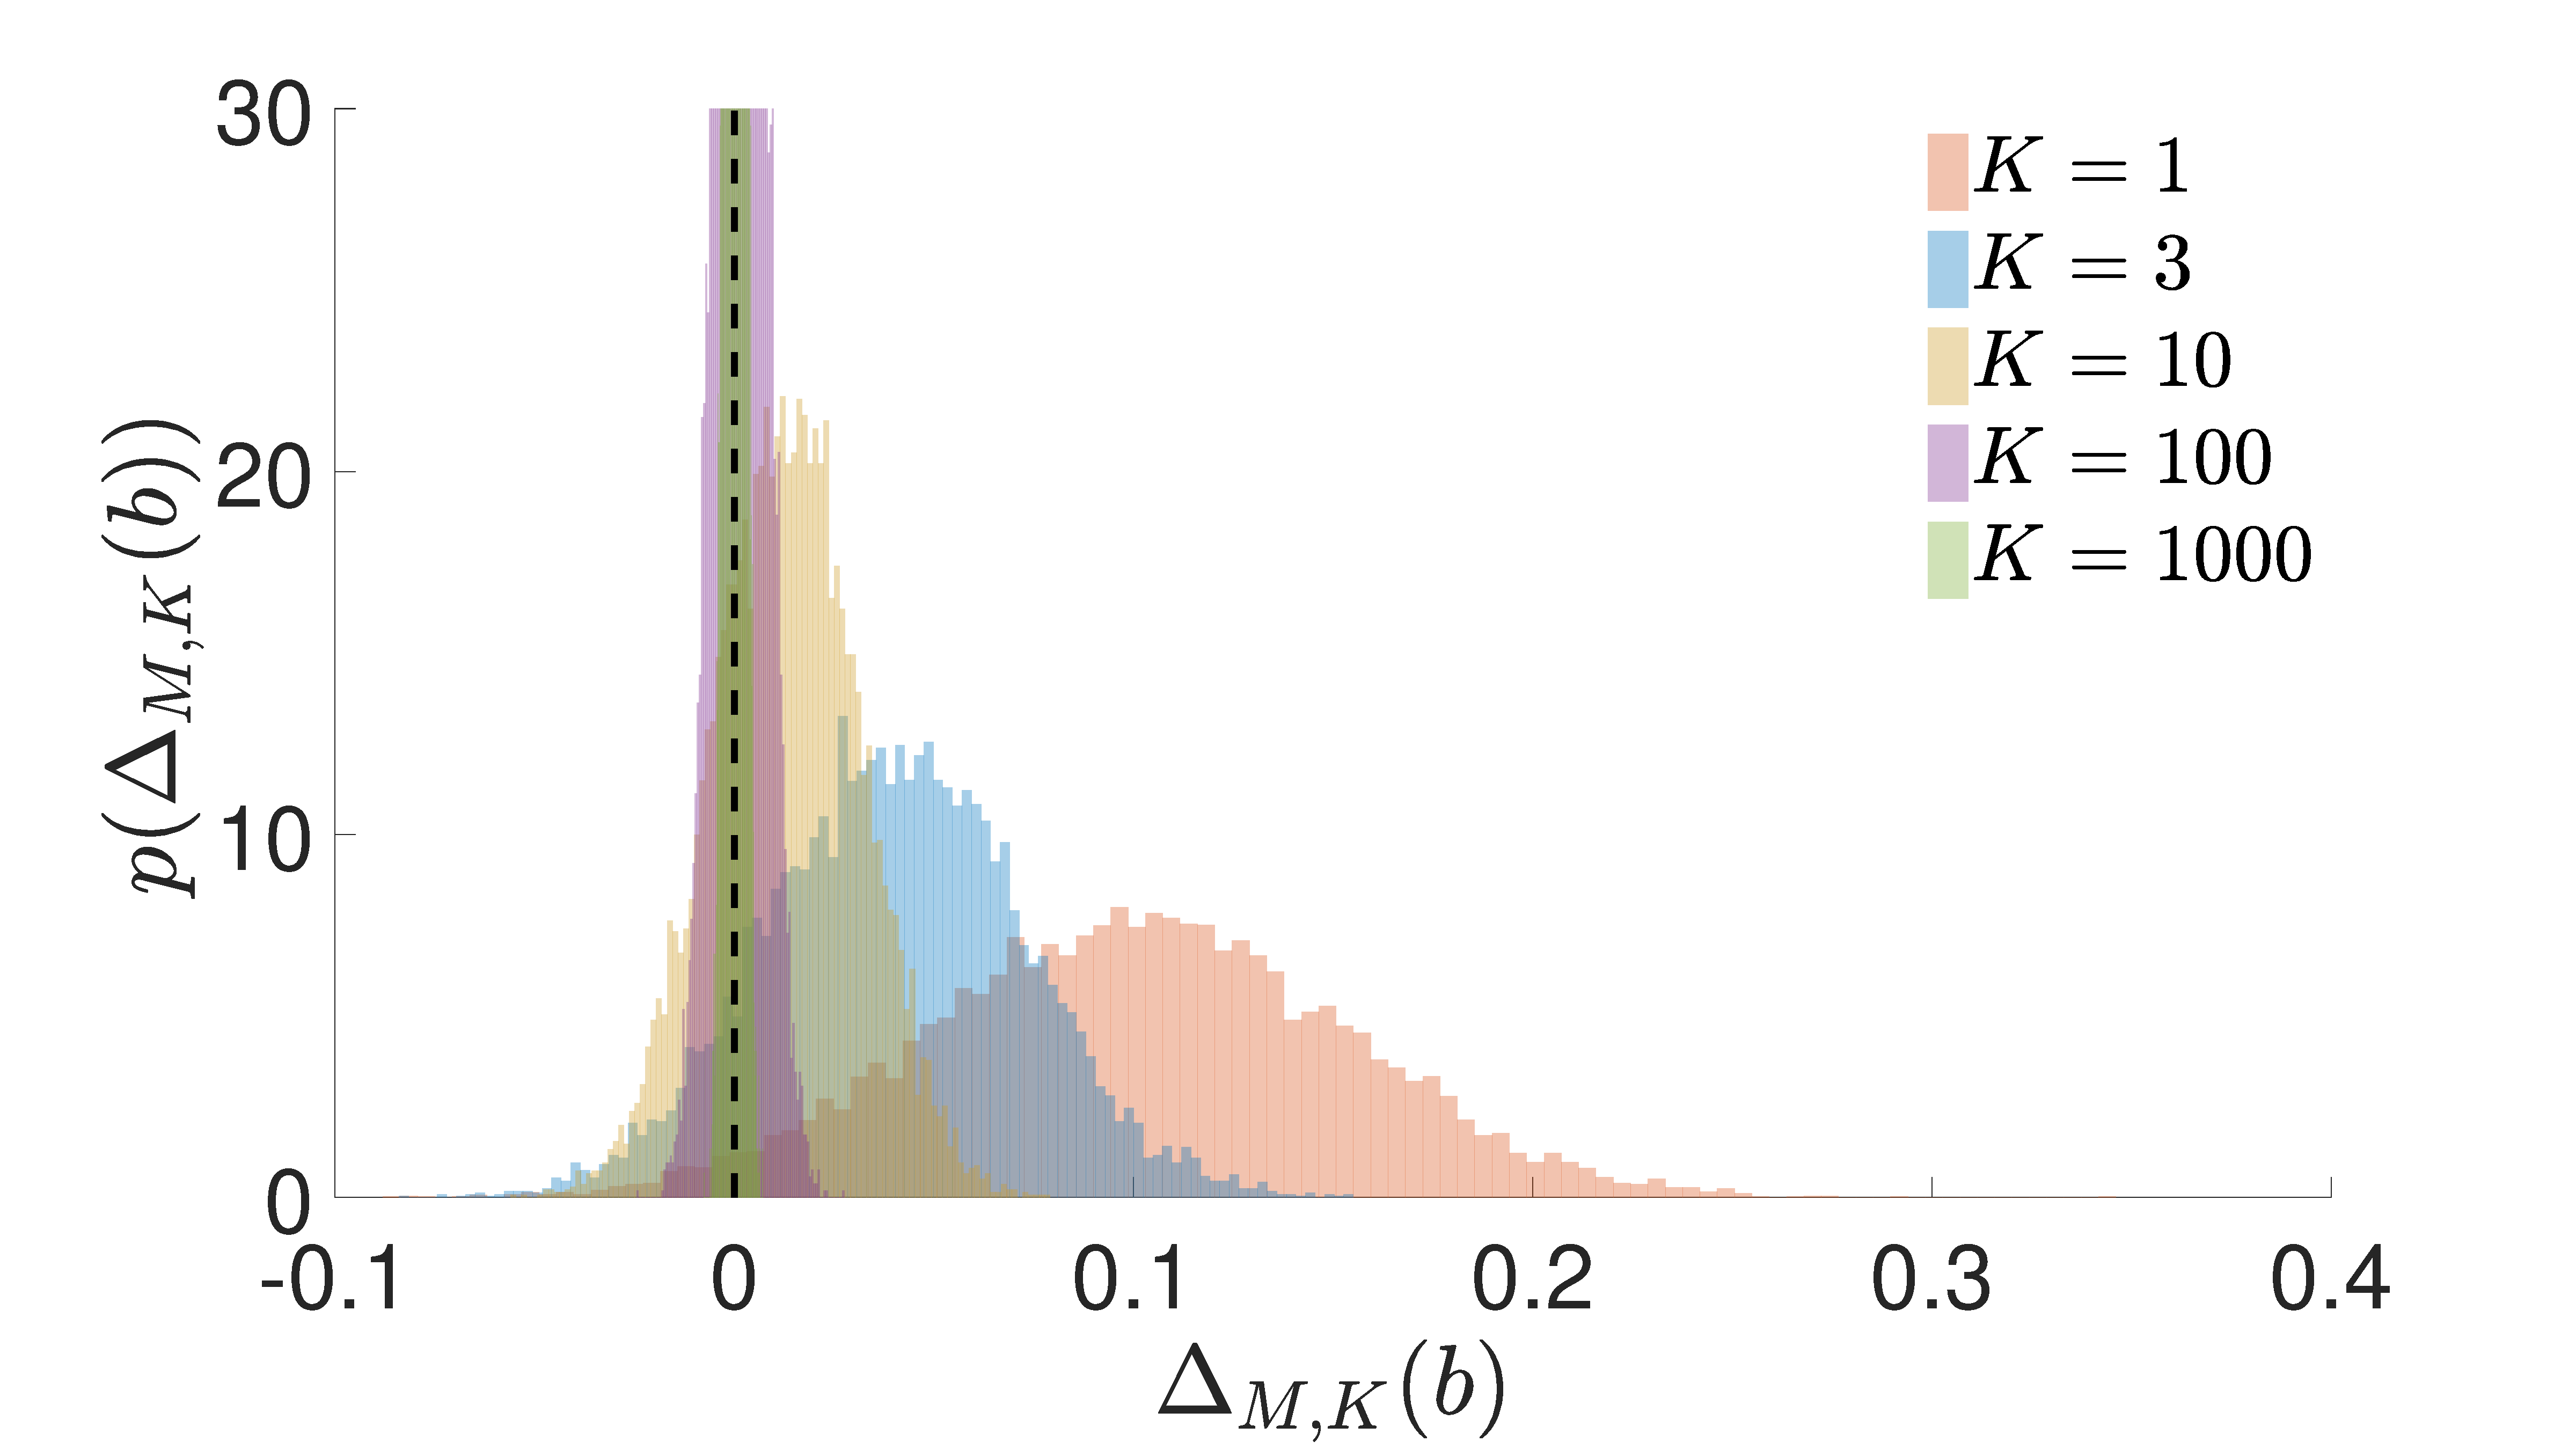
\includegraphics[width=\textwidth]{b_hist_IWAE}
%		\caption{\gls{IWAE} inference network gradient estimates \label{fig:snr/b_hist_iwae}}
%	\end{subfigure}
		\begin{subfigure}[b]{0.45\textwidth}
			\centering
			\includegraphics[width=\textwidth]{figures/tighter_bounds/b_hist_VAE}
			\caption{\gls{VAE} inference network gradient estimates \label{fig:snr/b_hist_vae}}
		\end{subfigure} ~~~~~~~~~~
%	\begin{subfigure}[b]{0.49\textwidth}
%		\centering
%		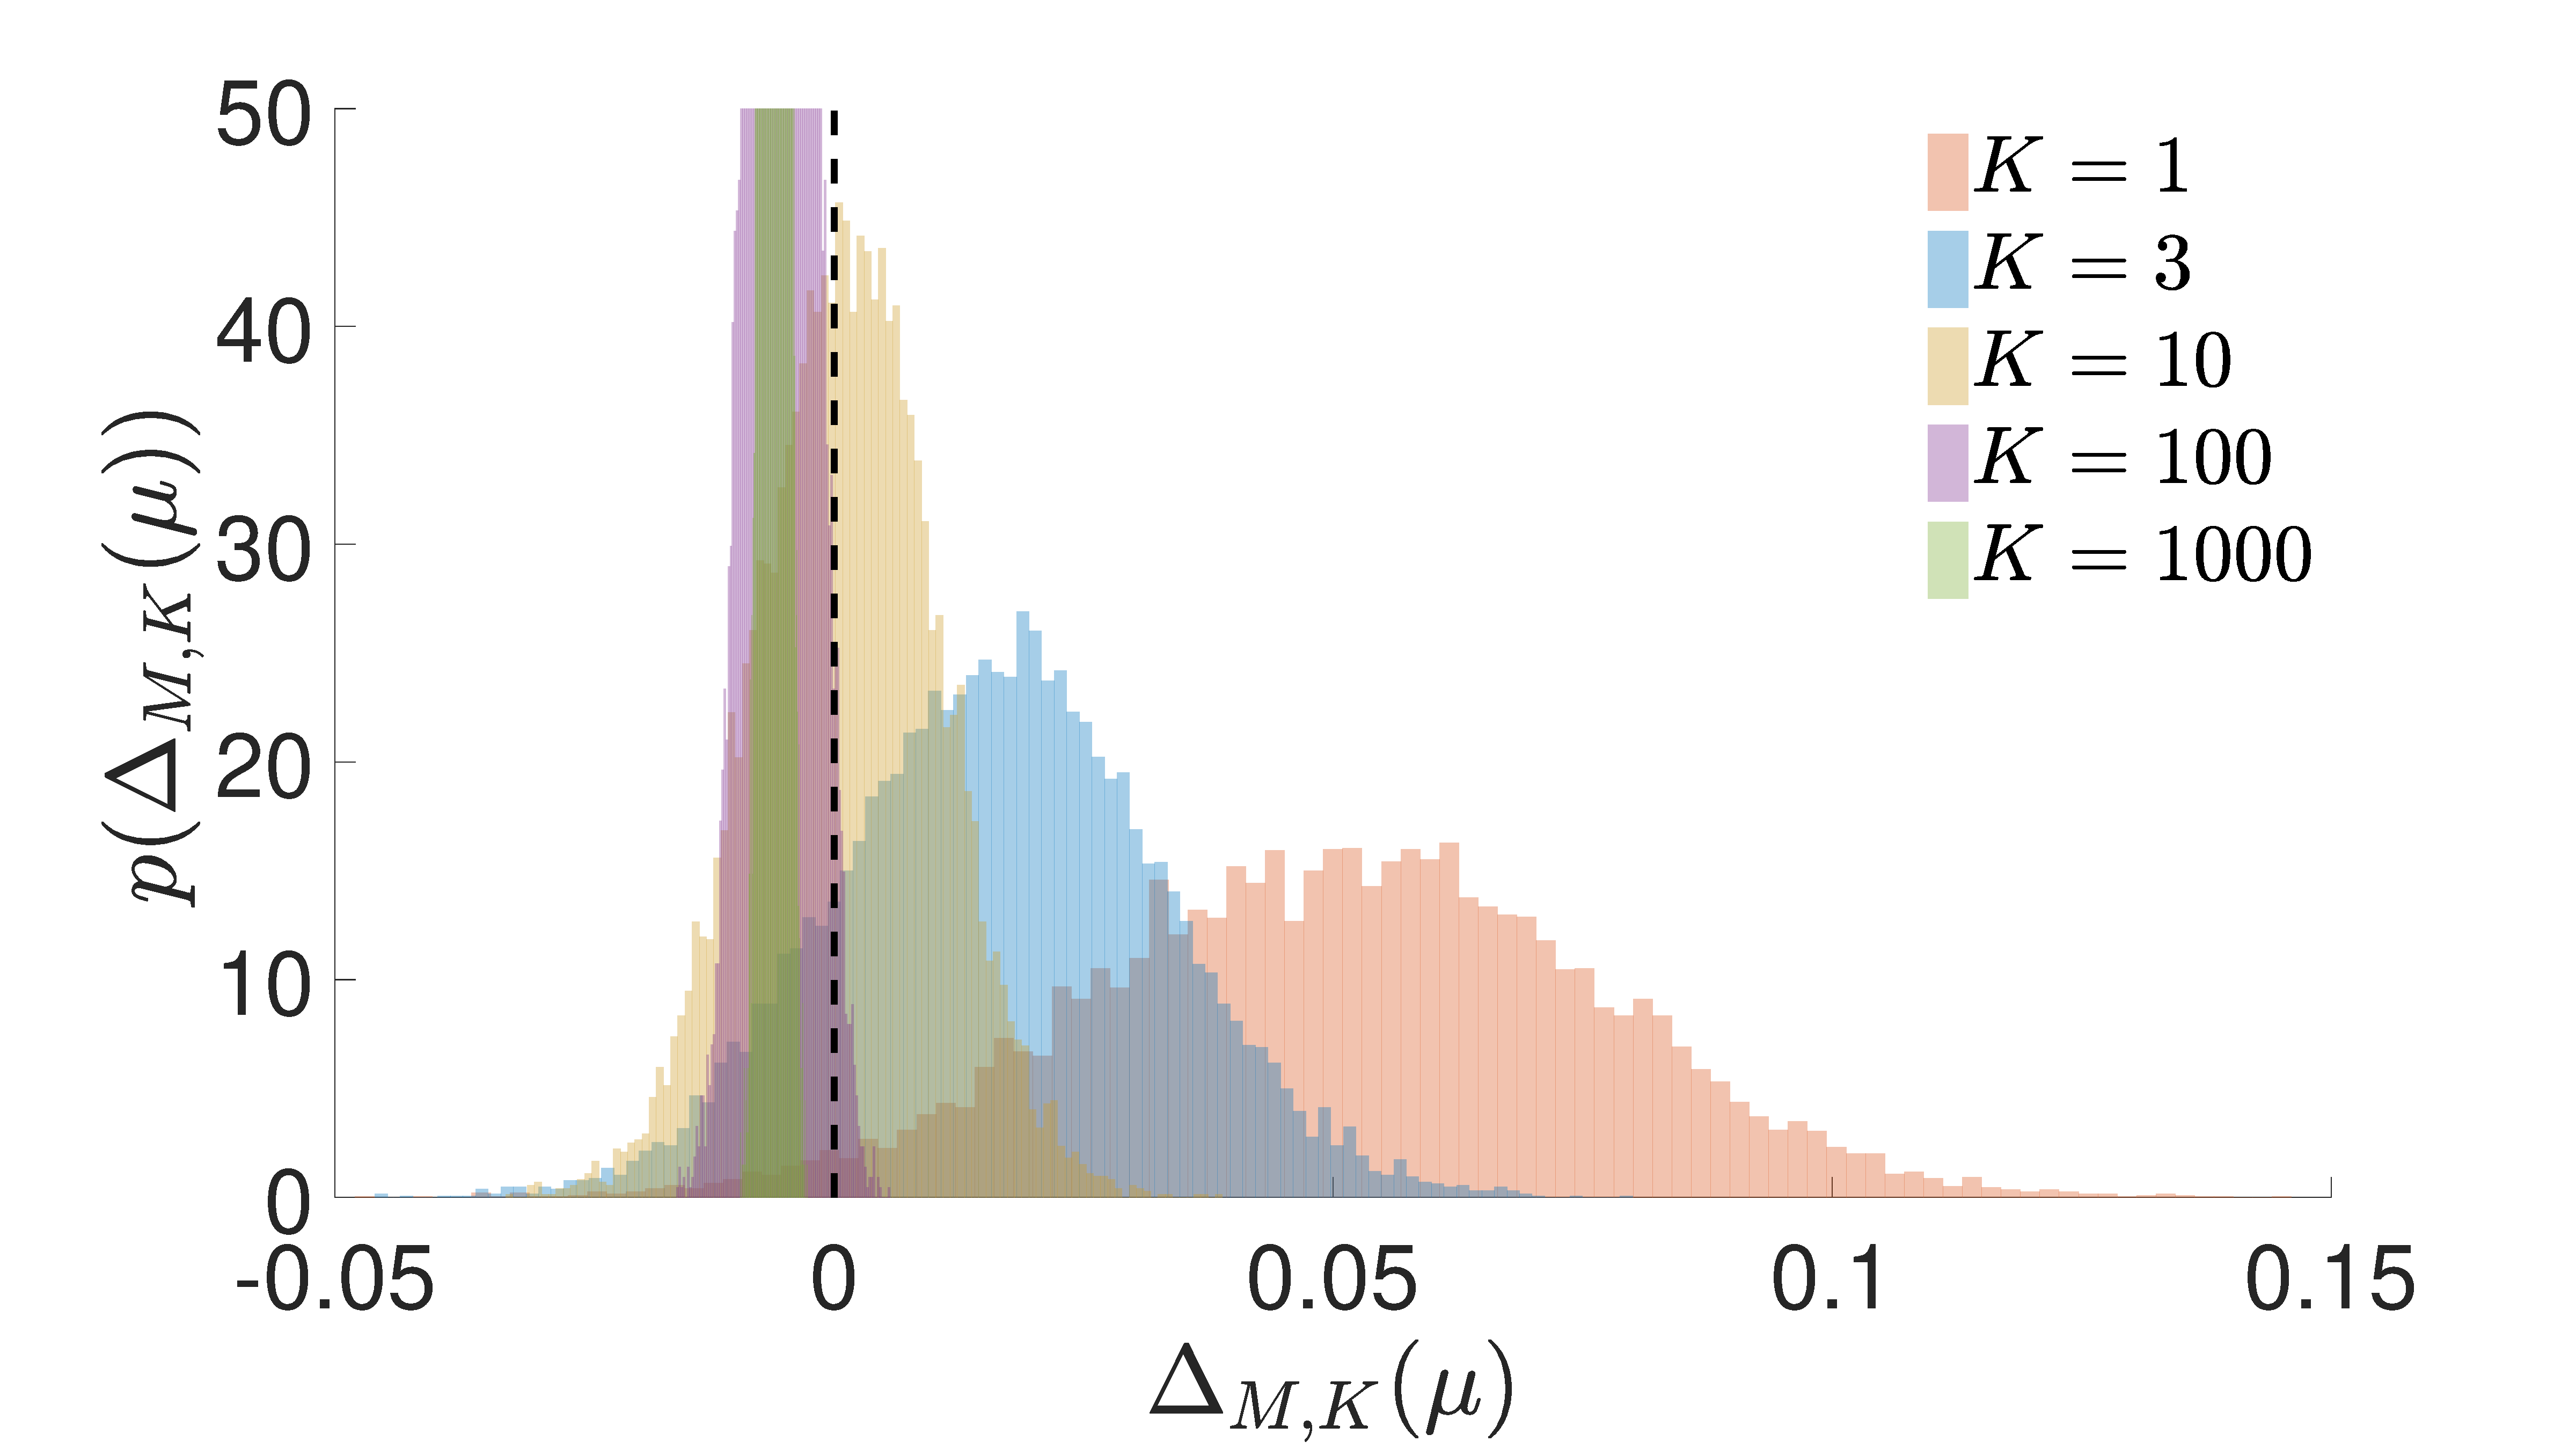
\includegraphics[width=\textwidth]{mu_hist_IWAE}
%		\caption{\gls{IWAE} generative network gradient estimates \label{fig:snr/mu_hist_iwae}}
%	\end{subfigure}
		\begin{subfigure}[b]{0.45\textwidth}
			\centering
			\includegraphics[width=\textwidth]{figures/tighter_bounds/mu_hist_VAE}
			\caption{\gls{VAE} generative network gradient estimates \label{fig:snr/mu_hist_vae}}
		\end{subfigure}
	\caption{Histograms of gradient estimates $\Delta_{M,K}$ for the generative network and 
		the	inference network using the \gls{VAE} ($K=1$) objectives with different values of $M$. \vspace{-12pt}
		\label{fig:snr/hists-vae}}
\end{figure*}

\subsection{Convergence of RMSE for Generative Network}
\label{sec:app:rmse}

\begin{wrapfigure}{r}{0.5\textwidth}
	\centering
	\vspace{-15pt}
	\includegraphics[width=0.47\textwidth]{figures/tighter_bounds/mse_mu}
	\vspace{-10pt}
	\caption{RMSE in $\mu$ gradient estimate to $\nabla_{\mu} \log Z$ 
		\label{fig:snr/rmse}}
	\vspace{-8pt}
\end{wrapfigure} 
As explained in the main paper, the SNR is not an entirely appropriate metric for
the generative network -- a low SNR is still highly problematic, but a high SNR
does not indicate good performance.
It is thus perhaps better to measure
the quality of the gradient estimates for the generative network by looking at the \gls{RMSE}
to $\nabla_{\mu} \log Z$, i.e. $\sqrt{\E \left[\lVert\Delta_{M,K}-\nabla_{\mu} \log Z\rVert_2^2\right]}$.
The convergence of this \gls{RMSE}  is shown in
Figure~\ref{fig:snr/rmse} where the solid lines are the \gls{RMSE} estimates using $10^4$ runs 
and the shaded regions
show the interquartile range of the individual estimates. We see that increasing 
$M$ in the \gls{VAE} reduces the variance
of the estimates but has negligible effect on the \gls{RMSE} due to the fixed bias.  On the
other hand,
we see that increasing $K$ leads to a monotonic improvement, initially improving
at a rate $O(1/K)$ (because the bias is the dominating term in this region),
before settling to the standard Monte Carlo convergence rate of $O(1/\sqrt{K})$
(shown by the dashed lines).

\subsection{Experimental Results for High Variance Regime}
\label{sec:hv}

\vspace{-4pt}

We now present empirical results for a case where our weights are higher variance. Instead
of choosing a point close to the optimum by offsetting parameters with a standard deviation of $0.01$, 
we instead offset using a standard deviation of $0.5$.  We further increased the proposal covariance to $I$
to make it more diffuse.  This is now a scenario where the model is far from its optimum and the proposal
is a very poor match for the model, giving very high variance weights.


We see that the behavior is the
same for variation in $M$, but somewhat distinct for variation in $K$.  
In particular, the \gls{SNR} and \textsc{dsnr} only decrease slowly with $K$ for the inference network, while increasing $K$ no longer has much benefit for the \gls{SNR} of the
inference network.
%Increasing $K$ now also has a remarkably similar impact on the \gls{SNR} and \textsc{dsnr} of
%the gradients of the generative network as on the
%inference network.  
It is clear that, for this
setup, the problem is very far from the asymptotic regime in $K$ such that our theoretical results no
longer directly apply.  Nonetheless, the high-level effect observed is still that the \gls{SNR} of 
the inference
network deteriorates, albeit slowly, as $K$ increases.

\begin{figure}[h]
	\centering
	\begin{subfigure}[b]{0.45\textwidth}
		\centering
		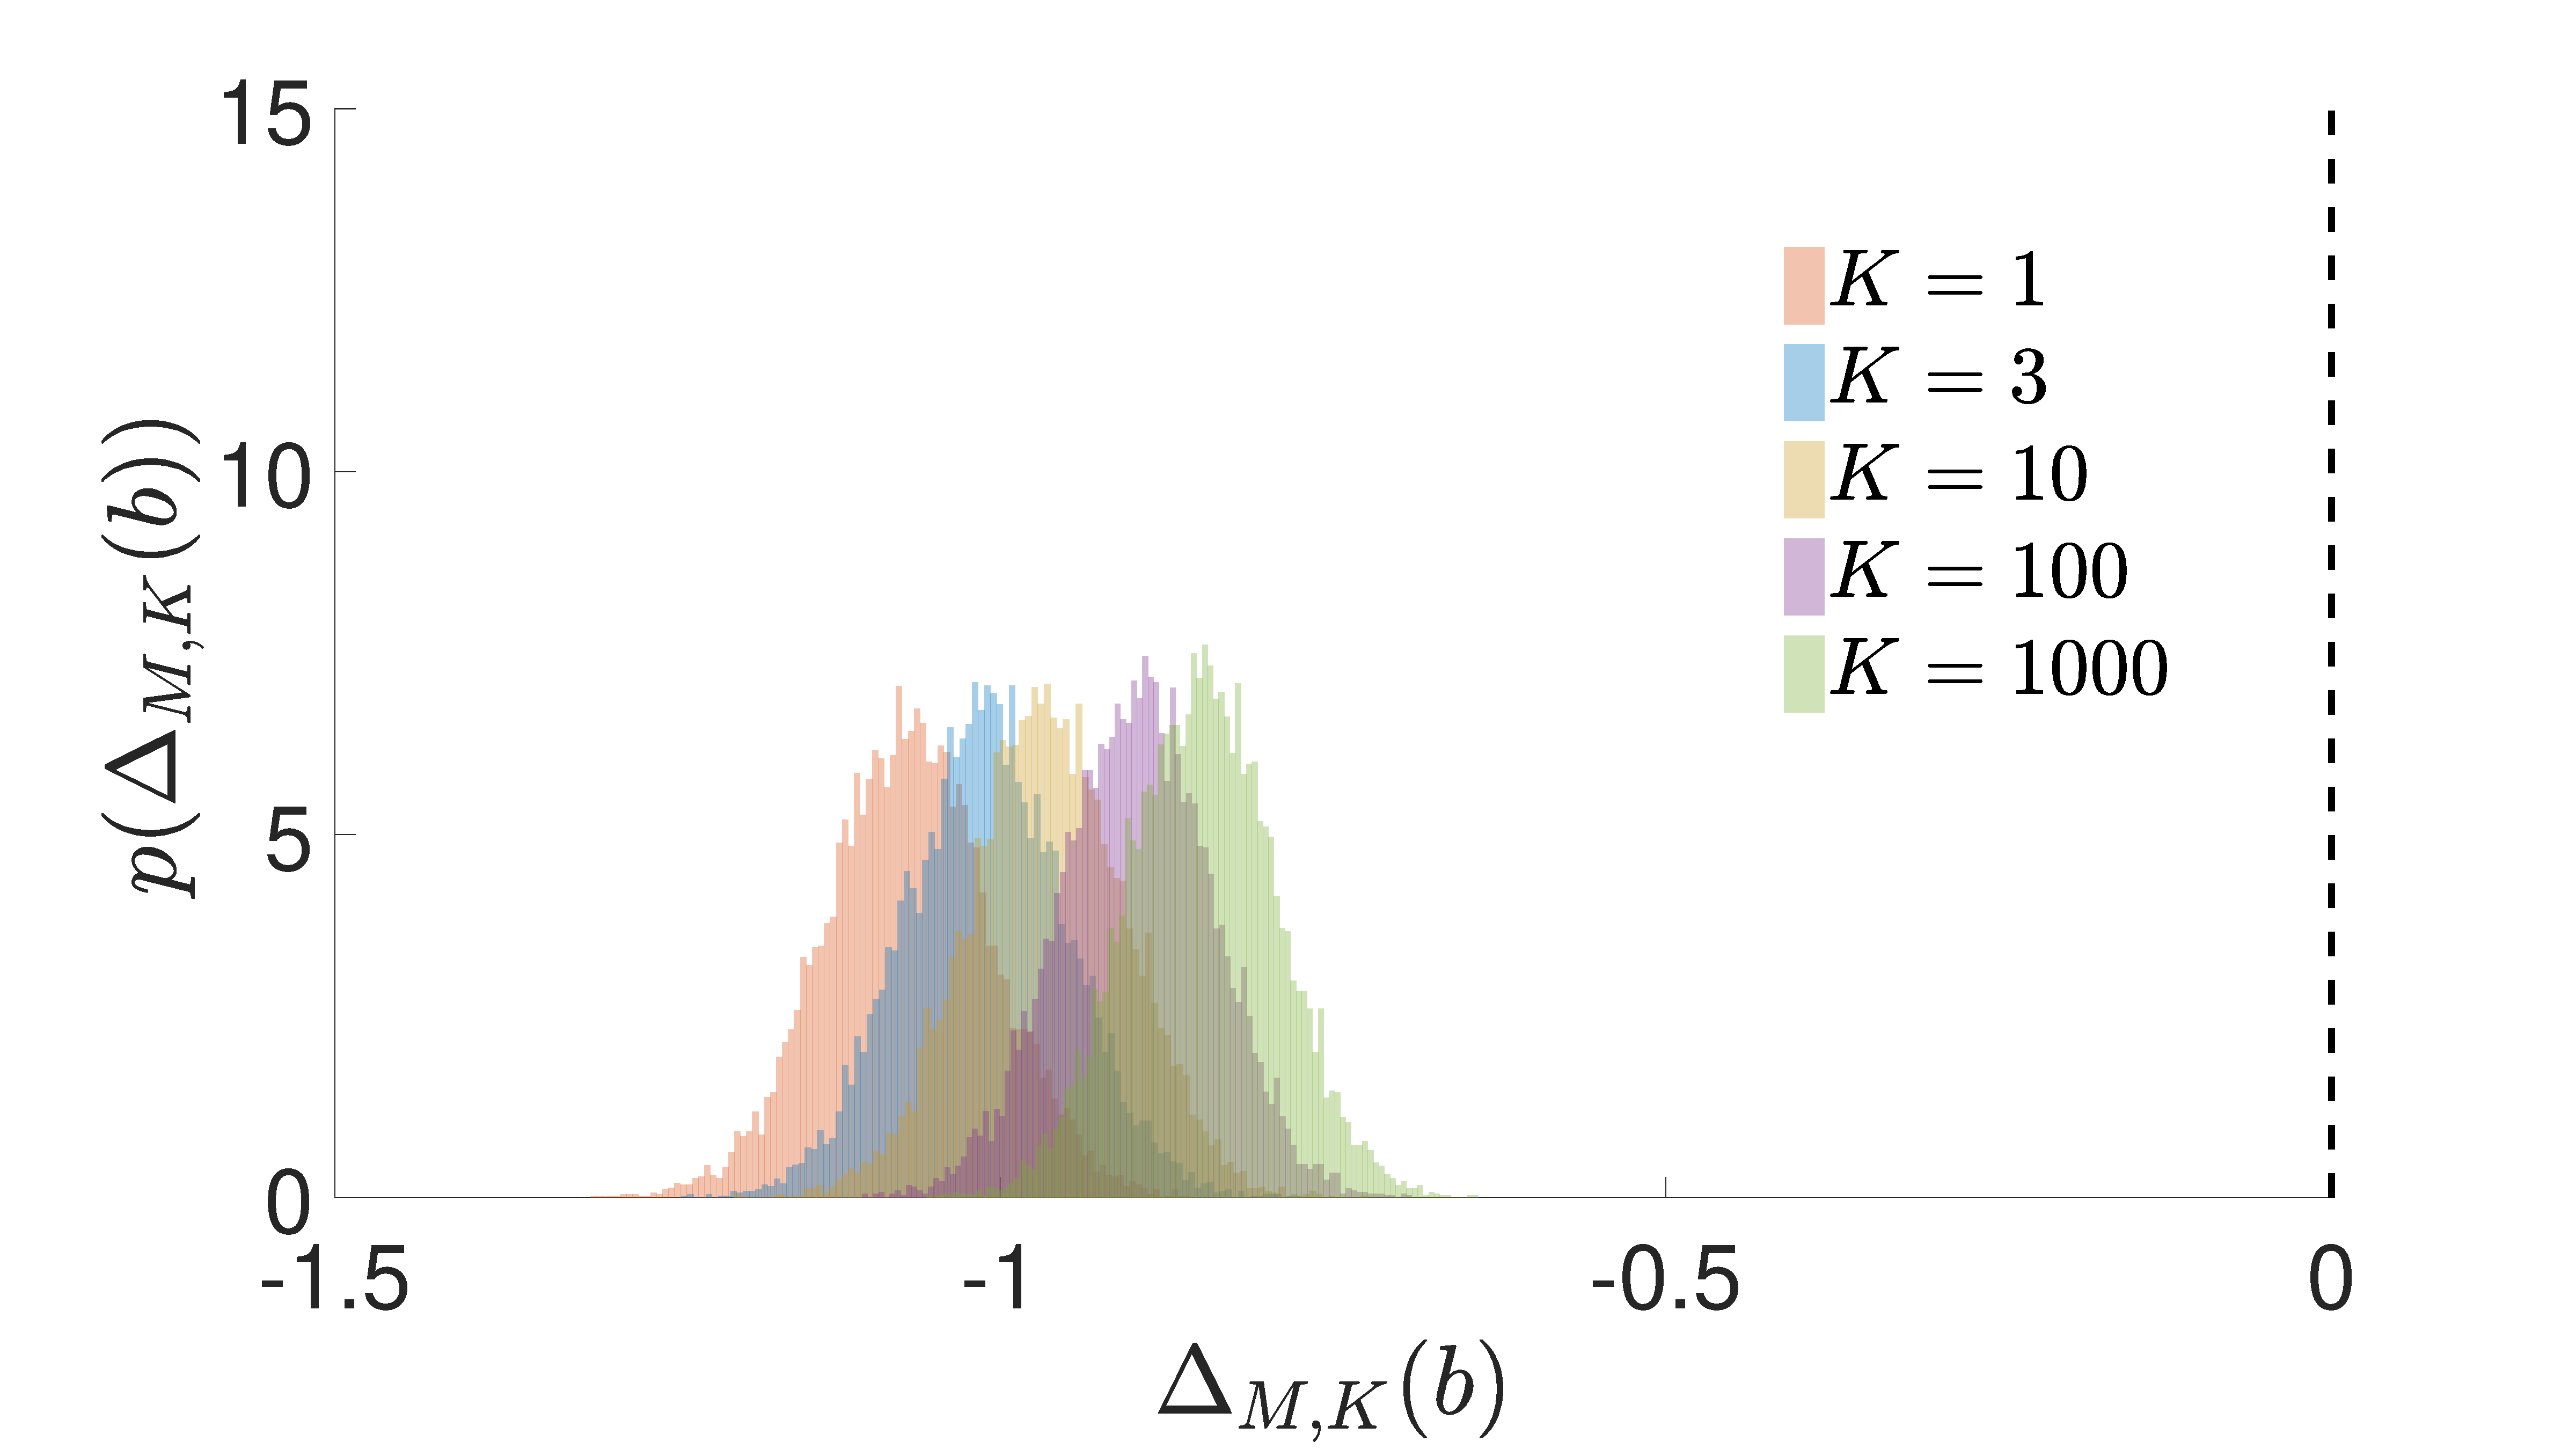
\includegraphics[width=\textwidth]{figures/tighter_bounds/hv_b_hist_IWAE}
		\caption{\gls{IWAE} inference network gradient estimates \label{fig:hv/b_hist_iwae}}
	\end{subfigure} ~~~~~~~~~~
	\begin{subfigure}[b]{0.45\textwidth}
		\centering
		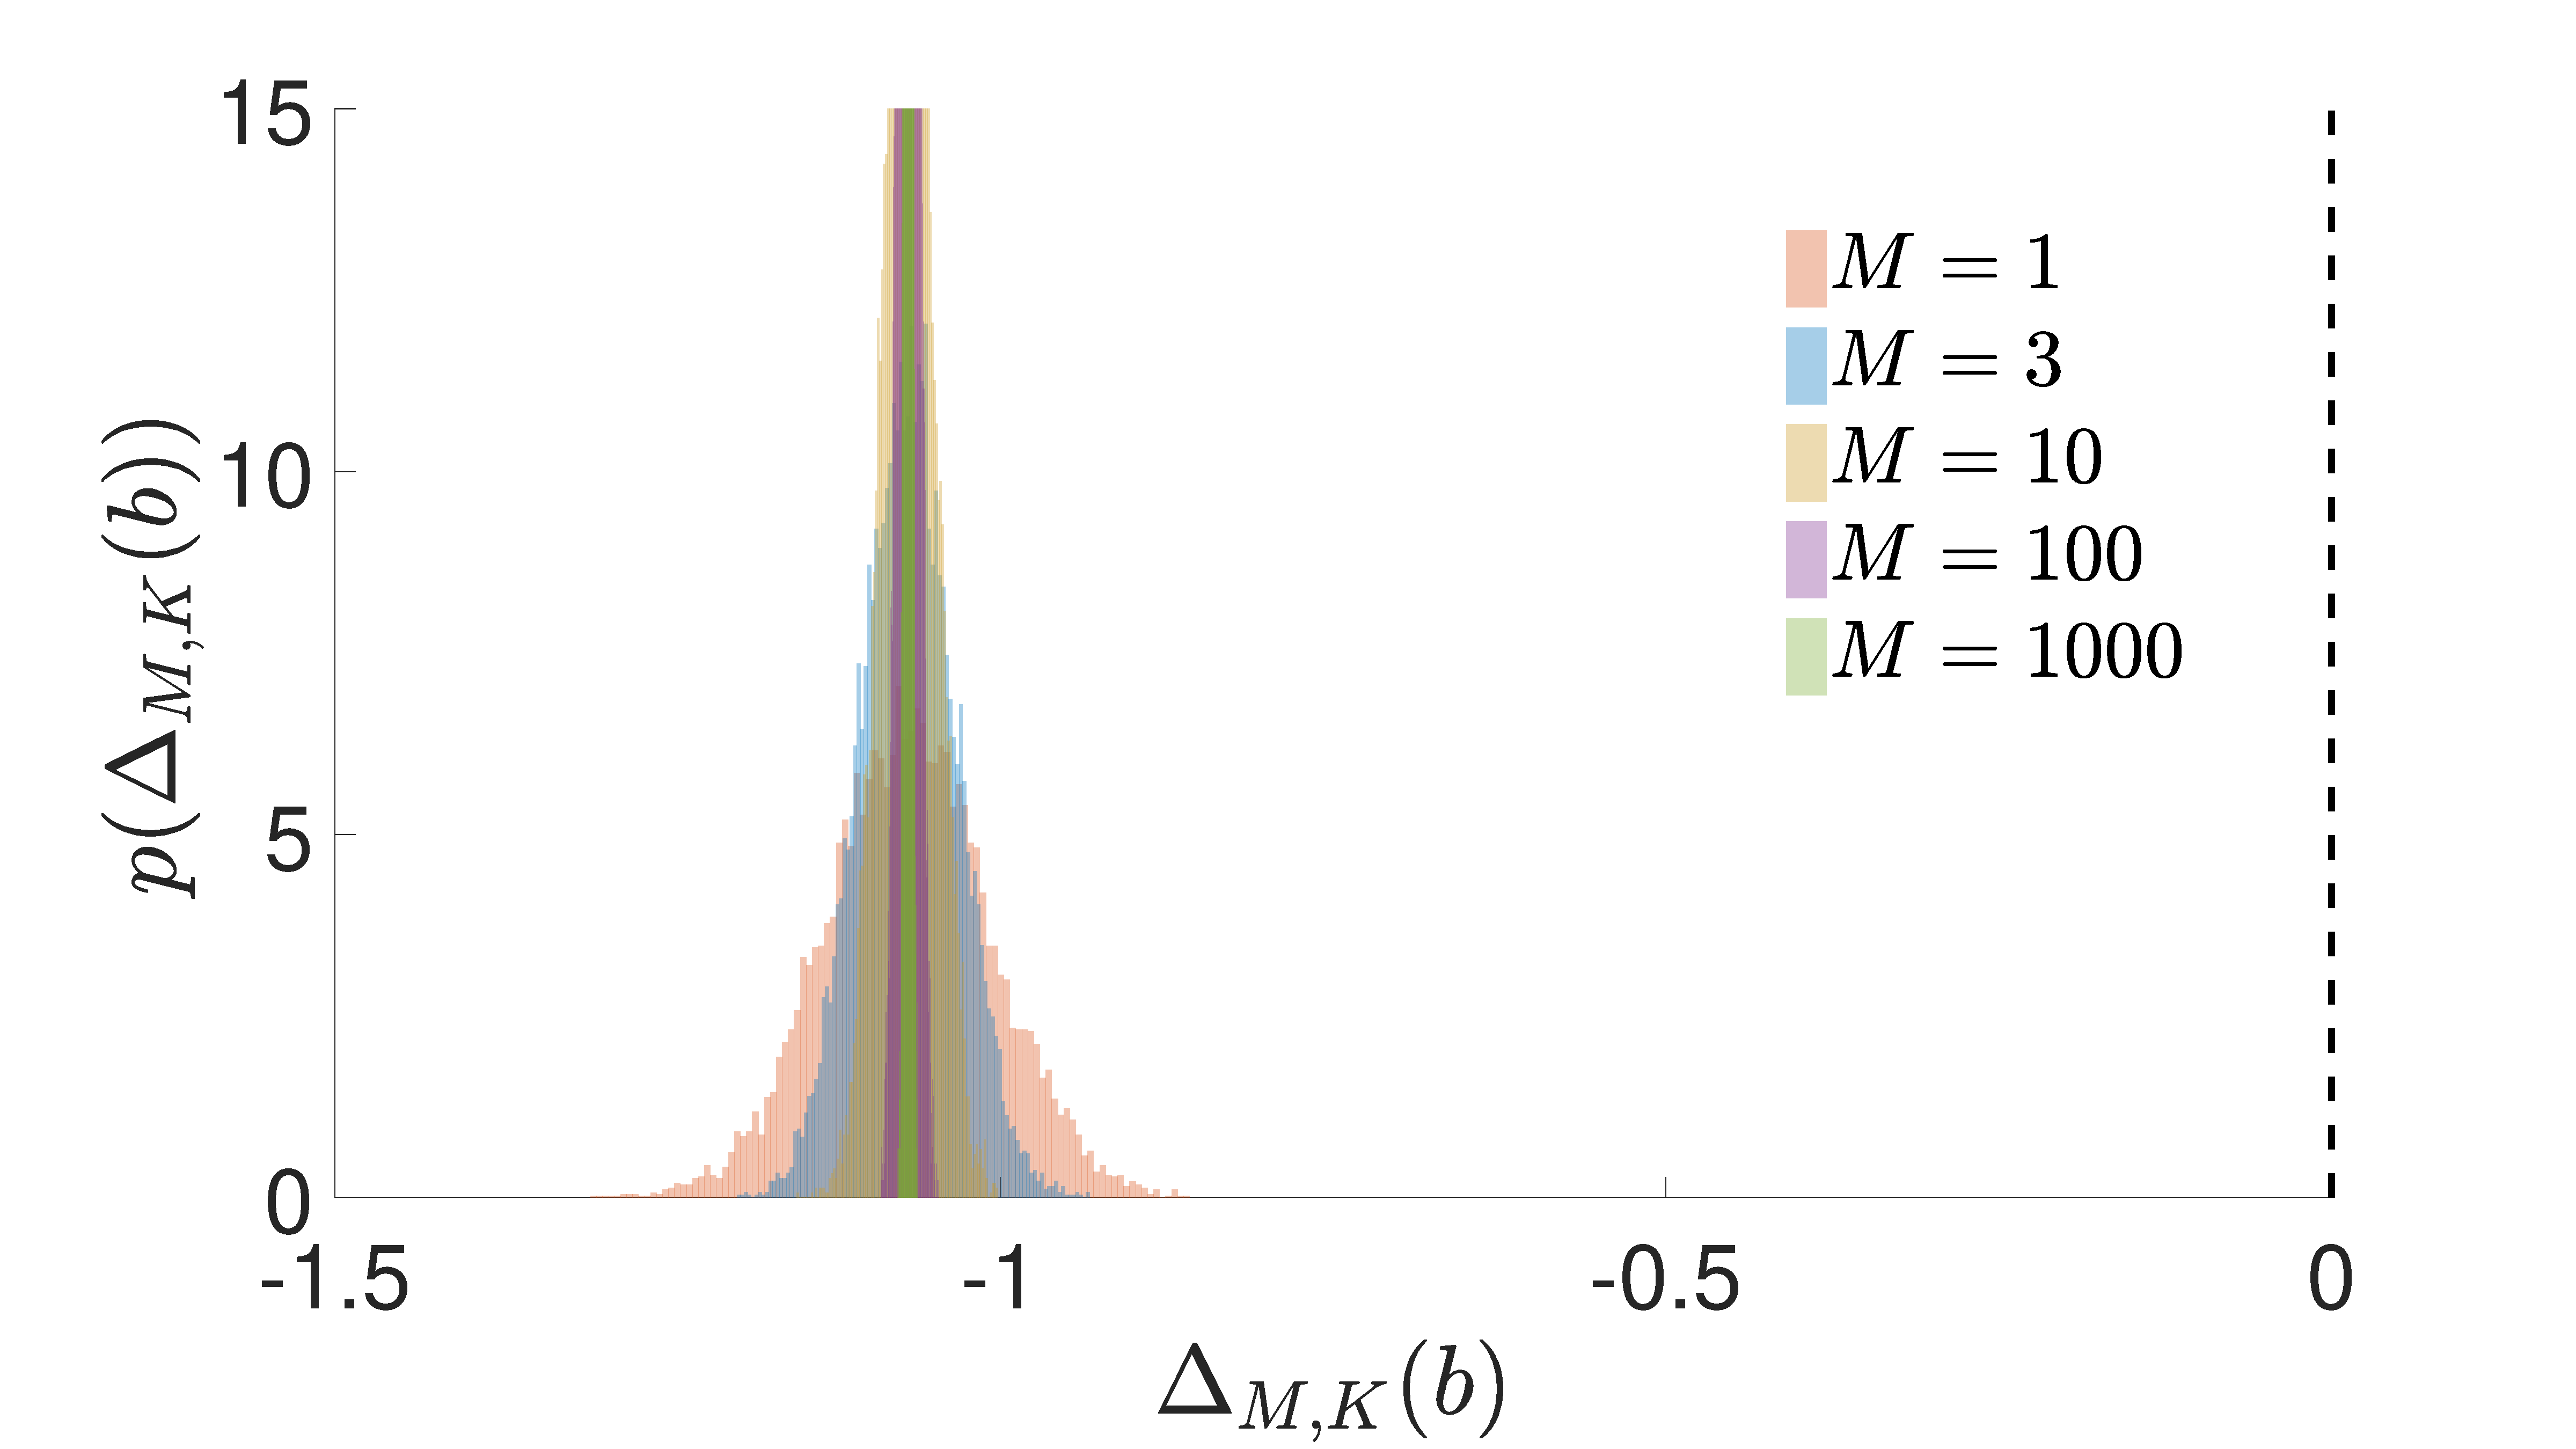
\includegraphics[width=\textwidth]{figures/tighter_bounds/hv_b_hist_VAE}
		\caption{\gls{VAE} inference network gradient estimates \label{fig:hv/b_hist_vae}}
	\end{subfigure}\\
	\begin{subfigure}[b]{0.45\textwidth}
		\centering
		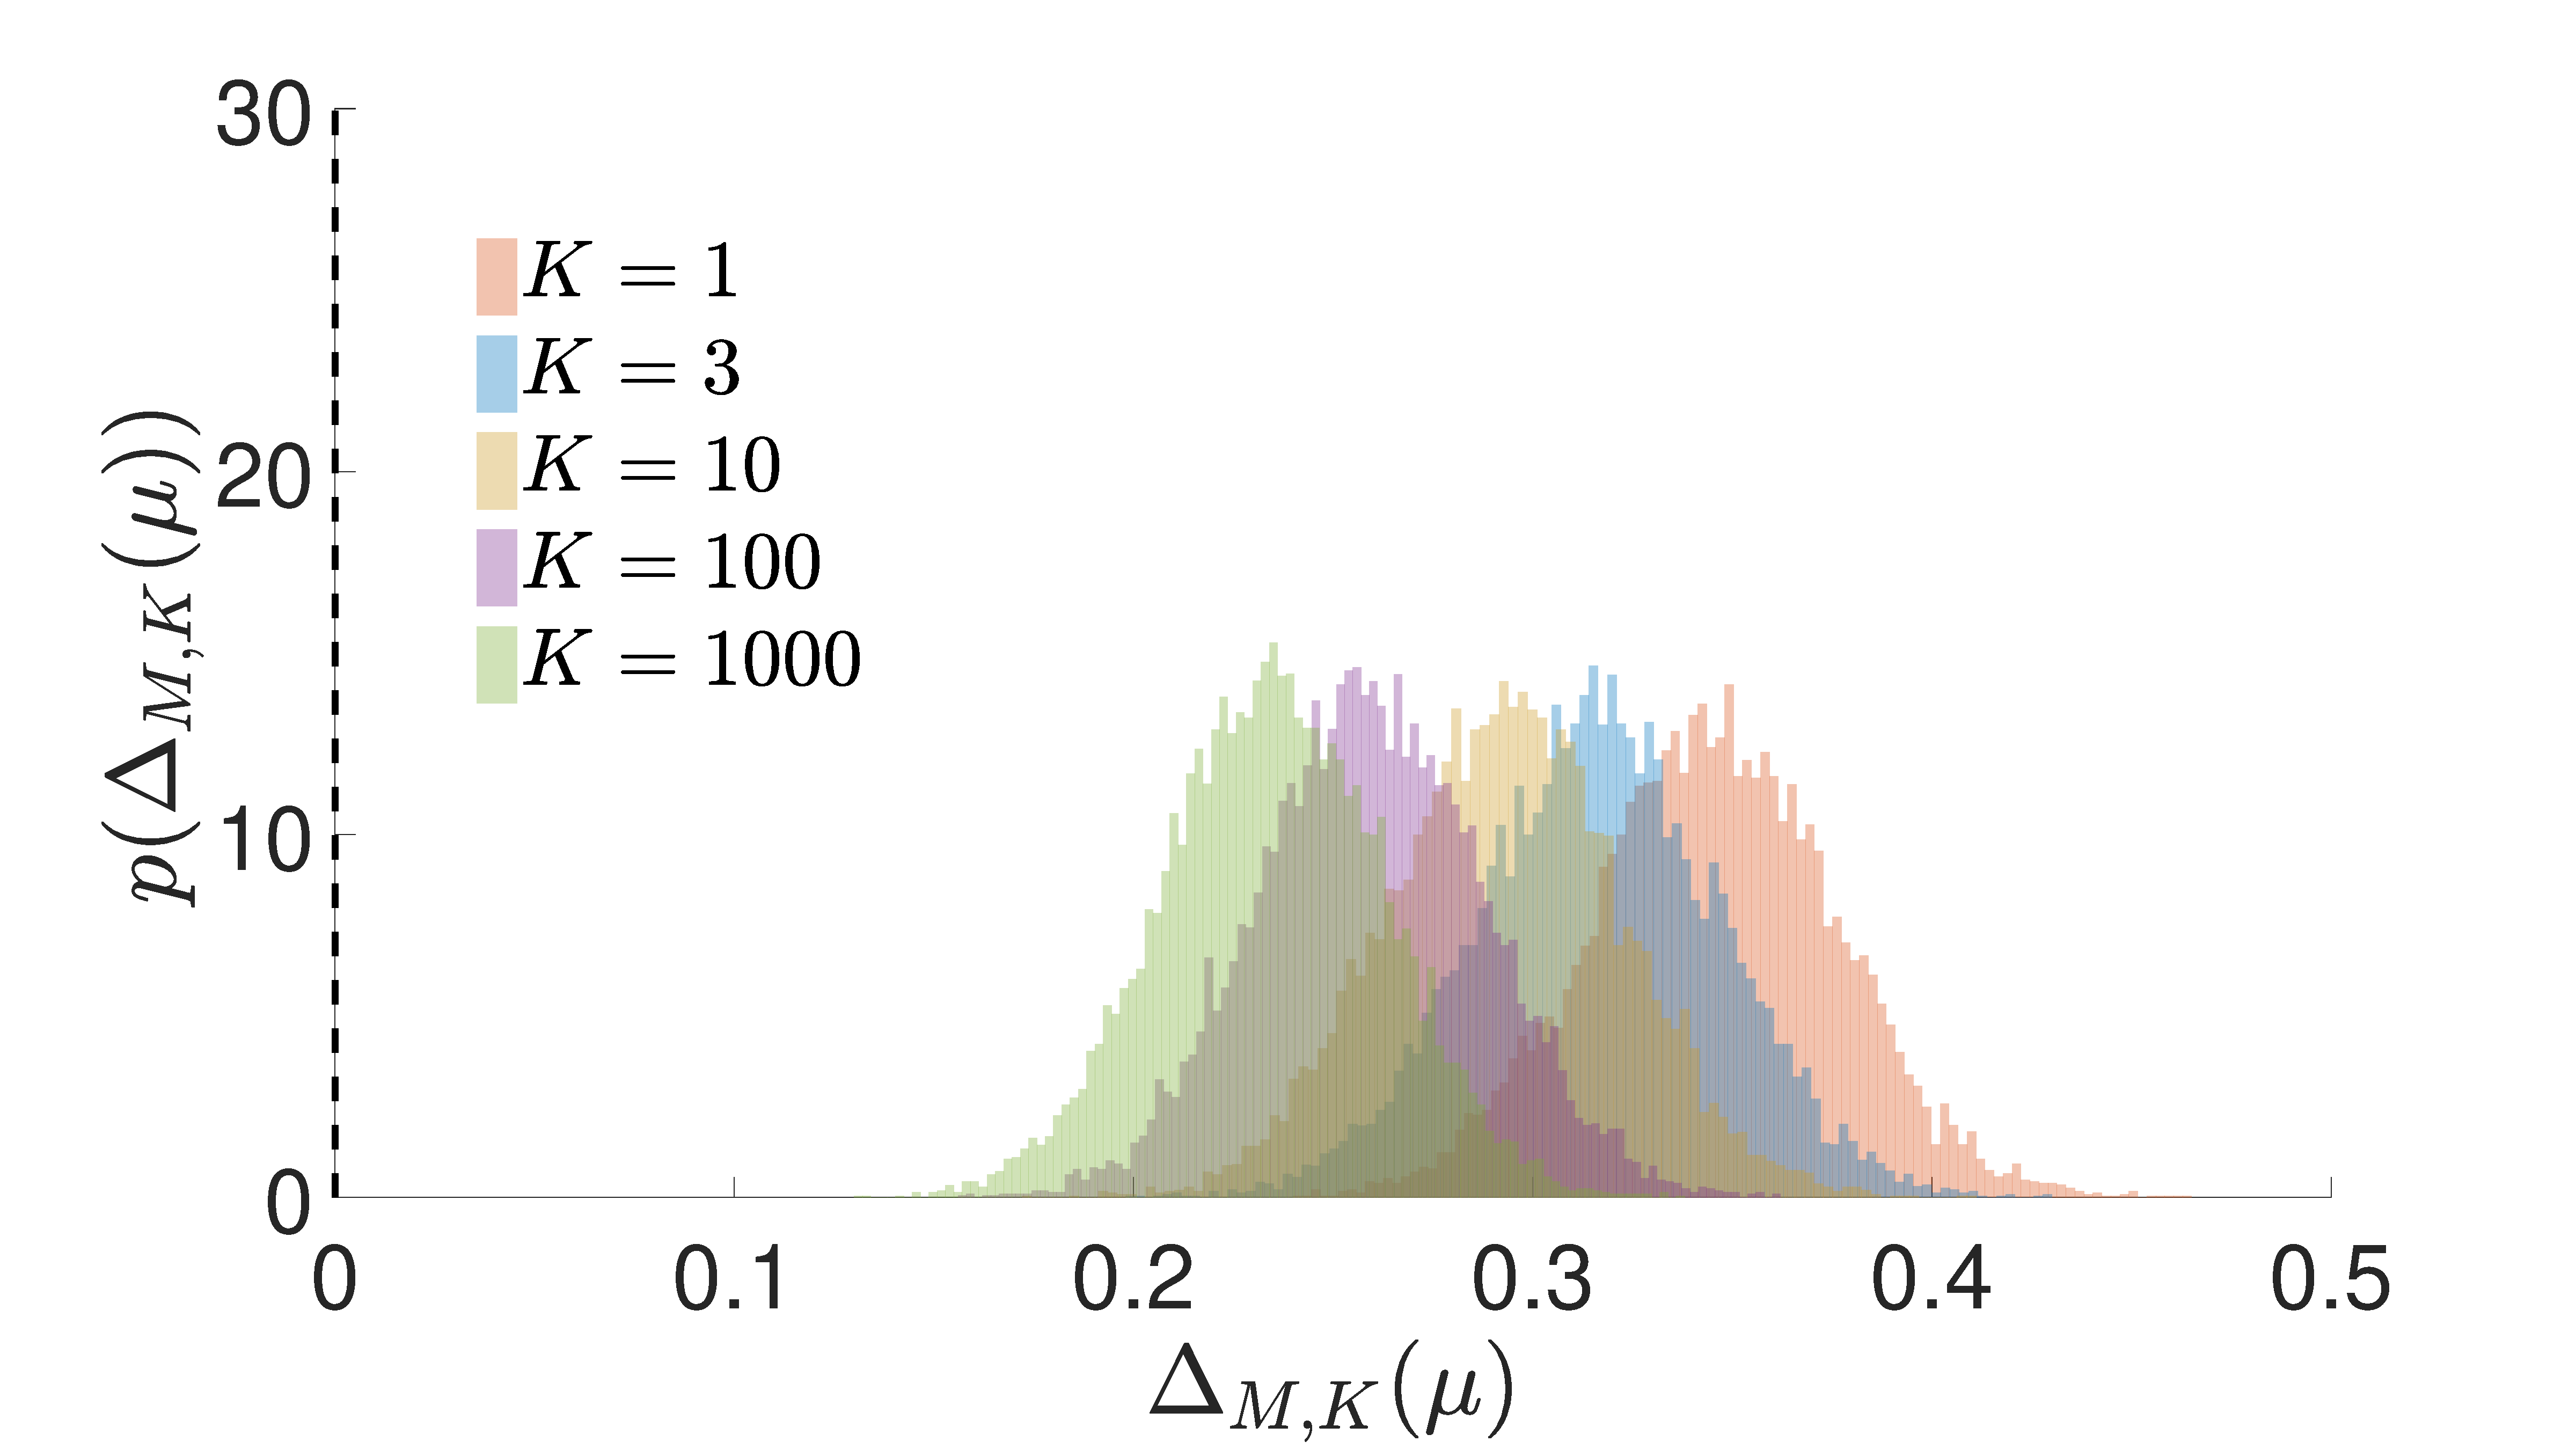
\includegraphics[width=\textwidth]{figures/tighter_bounds/hv_mu_hist_IWAE}
		\caption{\gls{IWAE} generative network gradient estimates \label{fig:hv/mu_hist_iwae}}
	\end{subfigure} ~~~~~~~~~~
	\begin{subfigure}[b]{0.45\textwidth}
		\centering
		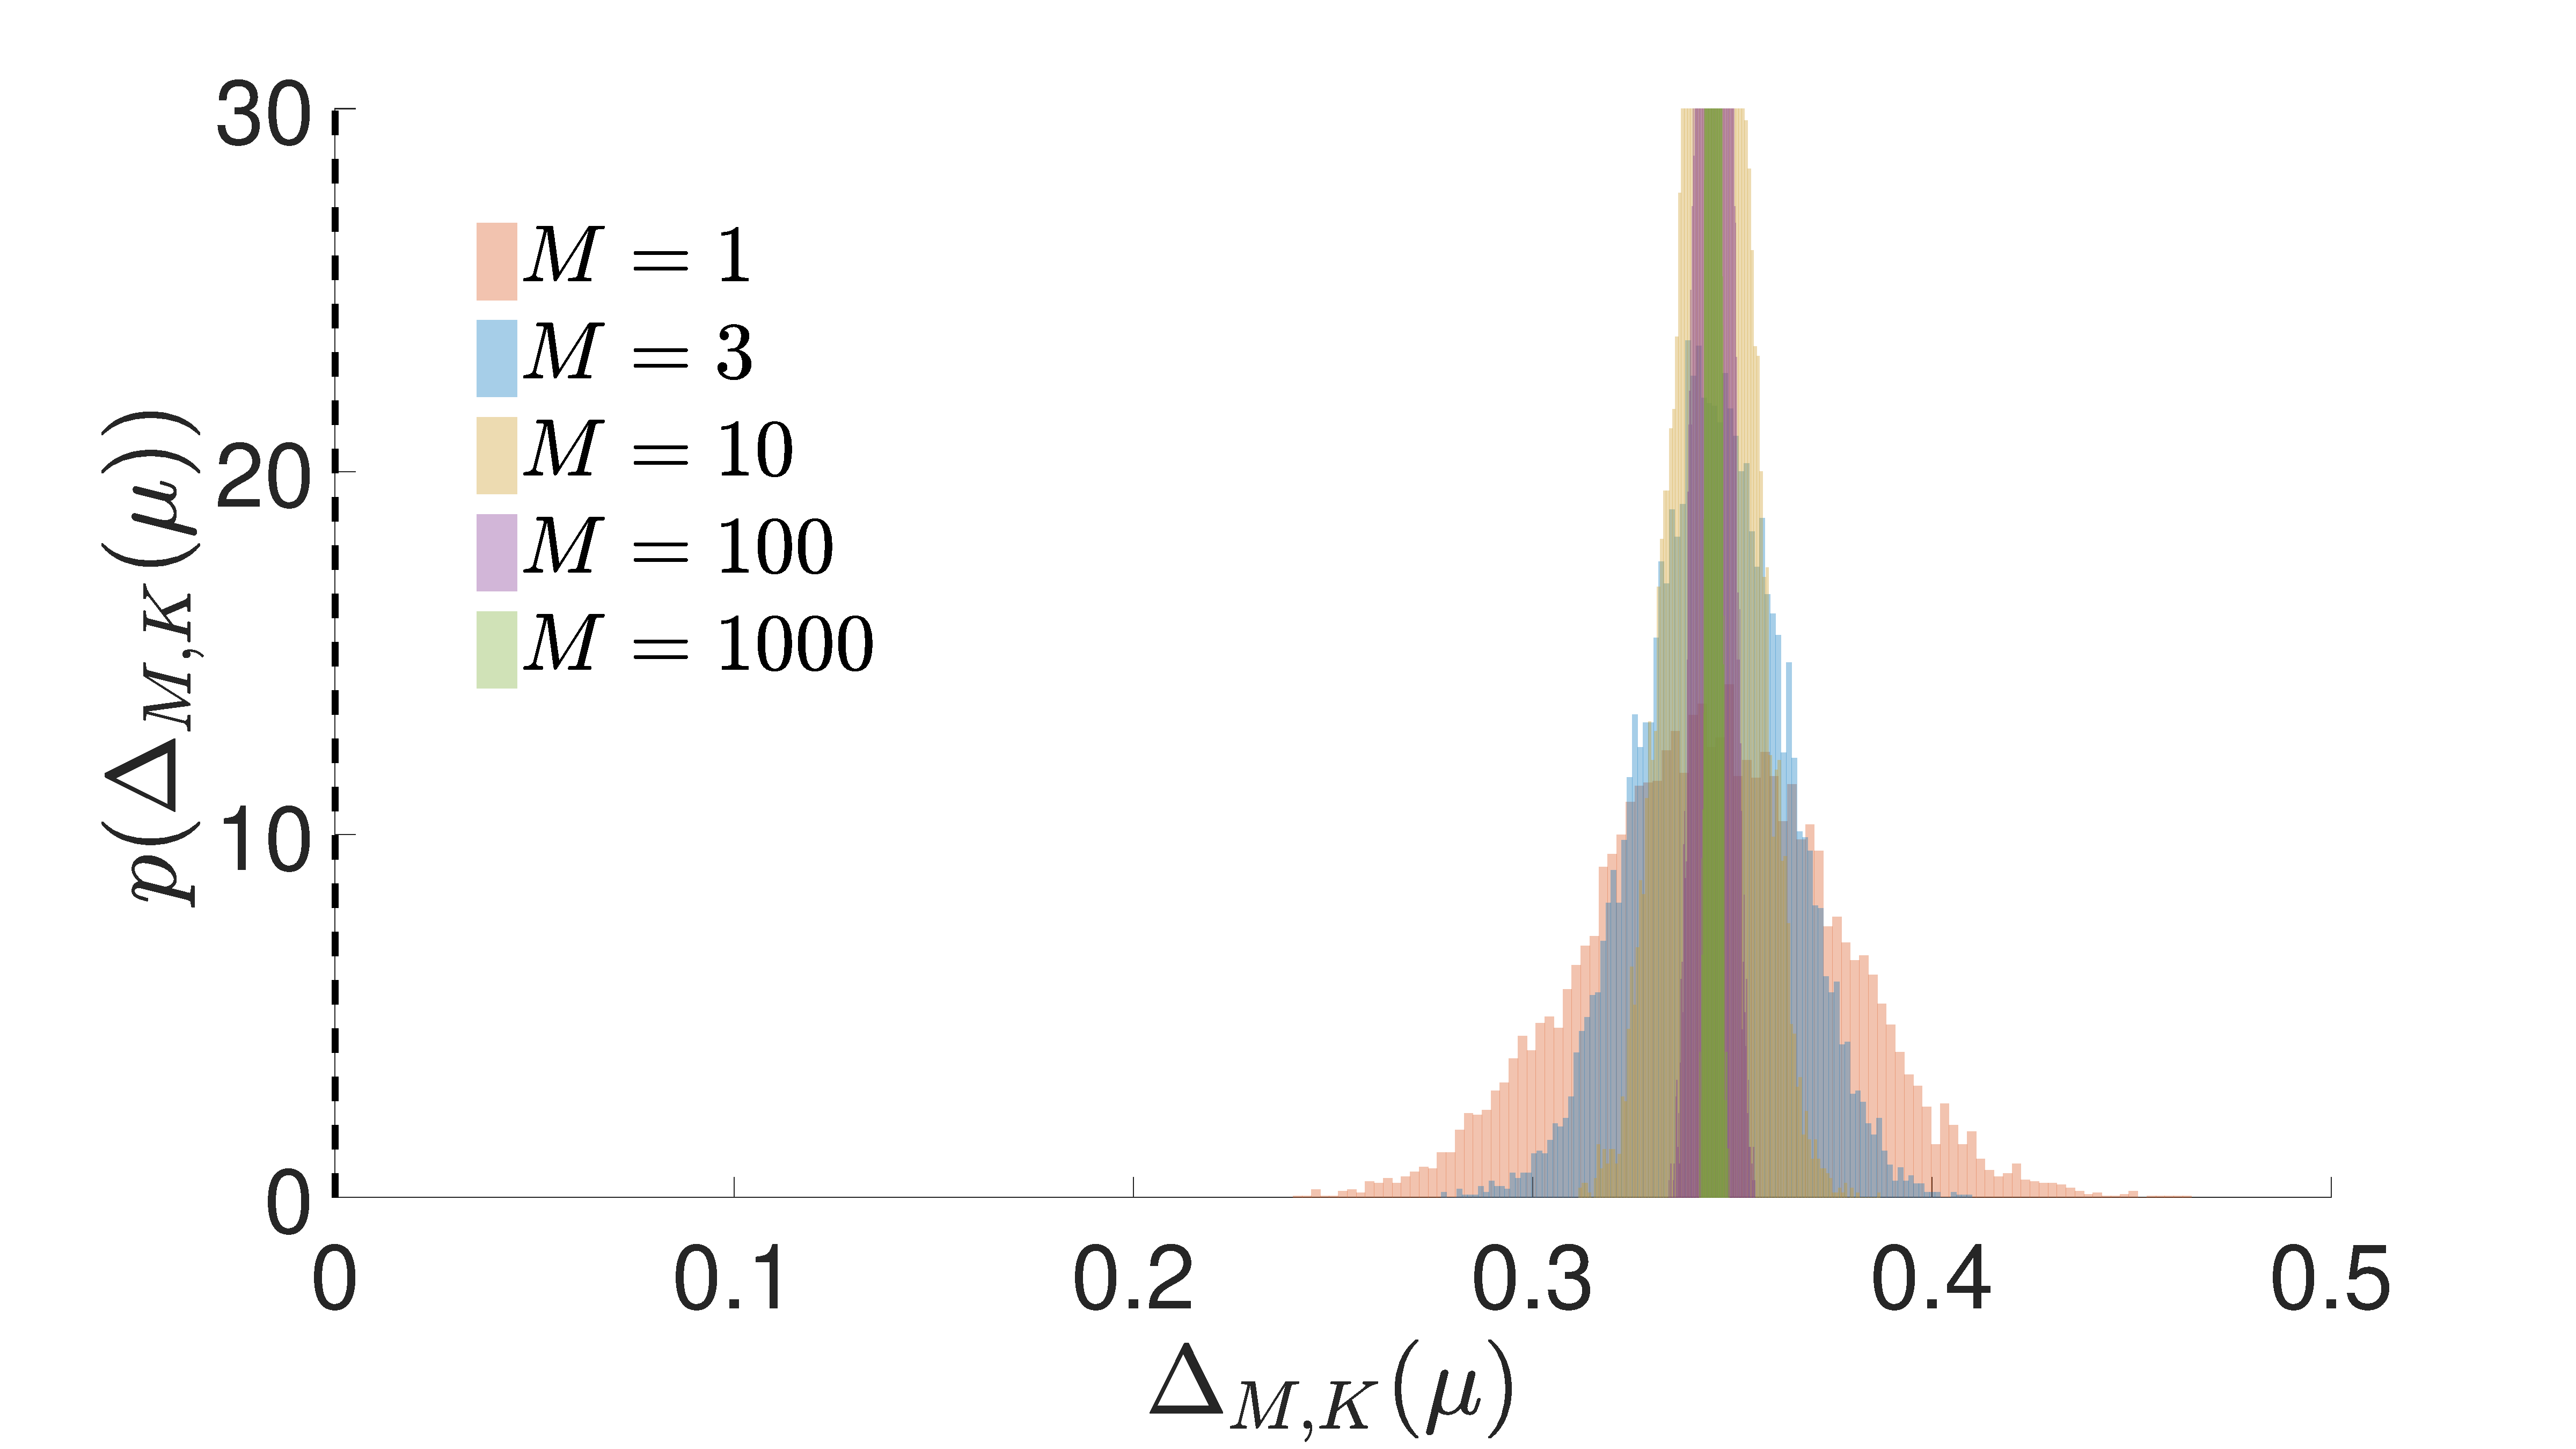
\includegraphics[width=\textwidth]{figures/tighter_bounds/hv_mu_hist_VAE}
		\caption{\gls{VAE} generative network gradient estimates \label{fig:hv/mu_hist_vae}}
	\end{subfigure}
	\caption{Histograms of gradient estimates as per Figure~\ref{fig:snr/hists}.
		\label{fig:hv/hists}
	\vspace{-4pt}}
\end{figure}

\begin{figure}[h]
	\centering
	\begin{subfigure}[b]{0.45\textwidth}
		\centering
		\includegraphics[width=\textwidth]{figures/tighter_bounds/hv_b_conv}
		\caption{Convergence of \gls{SNR} for inference network \label{fig:hv/b}}
	\end{subfigure} ~~~~~~~~~~
	\begin{subfigure}[b]{0.45\textwidth}
		\centering
		\includegraphics[width=\textwidth]{figures/tighter_bounds/hv_mu_conv}
		\caption{Convergence of \gls{SNR} for generative network\label{fig:hv/mu}}
	\end{subfigure}
	\caption{Convergence of signal-to-noise ratios of gradient estimates
		as per Figure~\ref{fig:snr/K_conv}.
		\label{fig:hv/K_conv}}
\end{figure}


\begin{figure}[h]
	\centering
	\begin{subfigure}[b]{0.45\textwidth}
		\centering
		\includegraphics[width=\textwidth]{figures/tighter_bounds/hv_snr_dir}
		\caption{Convergence of \textsc{dsnr} for inference network\label{fig:hv/snr_dir}}
	\end{subfigure}~~~~~~~~~~
	\begin{subfigure}[b]{0.45\textwidth}
		\centering
		\includegraphics[width=\textwidth]{figures/tighter_bounds/hv_snr_dir_mu}
		\caption{Convergence of \textsc{dsnr} for generative network\label{fig:hv/snr_dir_mu}}
	\end{subfigure}
	\caption{Convergence of directional signal-to-noise ratio of gradients estimates 
		as per Figure~\ref{fig:snr/extra}.
		\label{fig:hv/extra_end}}
\end{figure}

\begin{figure}[h]
	\centering
	\begin{subfigure}[b]{0.45\textwidth}
		\centering
		\includegraphics[width=\textwidth]{figures/tighter_bounds/hv_dir_snr_end}
		\caption{Convergence of \textsc{dsnr} for inference network\label{fig:snr/hv_snr_dir_end}}
	\end{subfigure} ~~~~~~~~~~
	\begin{subfigure}[b]{0.45\textwidth}
		\centering
		\includegraphics[width=\textwidth]{figures/tighter_bounds/hv_dir_snr_mu_end}
		\caption{Convergence of \textsc{dsnr} for generative network\label{fig:snr/hv_snr_dir_mu_end}}
	\end{subfigure}
	\caption{Convergence of directional signal-to-noise ratio of gradient estimates where the
		true gradient is taken as $\E \left[\Delta_{1,1000}\right]$ as per
		Figure~\ref{fig:snr/extra_end}.
		\label{fig:snr/hv_extra_end}}
\end{figure}
% !Tex root=tb_icml_2018.tex

\section{Convergence of Deep Generative Model for Alternative Parameter Settings}
\label{sec:app:exp-algs}

Figure~\ref{fig-app:mnistexpt/convergence} shows the convergence of the introduced algorithms under different
settings to those shown in Figure~\ref{fig:mnistexpt/convergence}. Namely we consider $M=4, K=16$ for~\gls{PIWAE} and~\gls{MIWAE} 
and $\beta = 0.05$ for~\gls{CIWAE}.  These settings all represent tighter bounds than those of the main paper.
Similar behavior is seen in terms of the~\gls{IWAE}-64 metric for all algorithms.  \gls{PIWAE} produced
similar mean behavior for all metrics, though the variance was noticeably increased for $\log \hat{p}(x)$.
For~\gls{CIWAE} and~\gls{MIWAE}, we see that the parameter settings represent an explicit trade-off between
the generative network and the inference network:  $\log \hat{p}(x)$ was noticeably increased for both, matching
that of~\gls{IWAE}, while $-\textsc{KL}(Q_{\phi}(z \given x) || P_{\theta}(z \given x))$ was reduced.
Critically, we see here that, as observed for~\gls{PIWAE} in the main paper,~\gls{MIWAE} and~\gls{CIWAE} are able to
match the generative model performance of~\gls{IWAE} whilst improving the KL metric, indicating that they have learned
better inference networks.

\begin{figure*}[h]
	\centering
   	\begin{subfigure}[b]{0.33\textwidth}
        \centering
        \includegraphics[width=\textwidth]{figures/tighter_bounds/optim_convergence_IWAE_64}
        \caption{\textsc{IWAE}$_{64}$ \label{fig-app:mnistexpt/convergence/iwae64}}
    \end{subfigure}
	\begin{subfigure}[b]{0.33\textwidth}
		\centering
		\includegraphics[width=\textwidth]{figures/tighter_bounds/optim_convergence_log_p(x)}
		\caption{$\log \hat{p}(x)$ \label{fig-app:mnistexpt/convergence/logpx}}
	\end{subfigure}
	\begin{subfigure}[b]{0.33\textwidth}
		\centering
		\includegraphics[width=\textwidth]{figures/tighter_bounds/optim_convergence_KL}
		\caption{$-\mathrm{KL}(Q_{\phi}(z \given x) || P_{\theta}(z \given x))$ \label{fig-app:mnistexpt/convergence/kl}}
	\end{subfigure}
	\caption{Convergence of different evaluation metrics for each method.  Plotting conventions as per
		 Figure~\ref{fig:mnistexpt/convergence}.
		\vspace{-12pt}  \label{fig-app:mnistexpt/convergence}}
\end{figure*}
% !Tex root=./tb_icml_2018.tex

\section{Convergence of Toy Gaussian Problem}
\label{sec:app:toy-Gauss}

We finish by assessing the effect of the outlined changes in the quality
of the gradient estimates on the final optimization for our toy Gaussian problem.  Figure~\ref{fig:snr/hd_gaussian}
shows the convergence of running Adam~\citep{kingma2014adam} to optimize $\mu$, $A$, 
and $b$.  This suggests that the effects observed predominantly transfer to the overall
optimization problem.  Interestingly, setting $K=1$ and $M=1000$ gave the best performance
on learning not only the inference network parameters, but also the generative network
parameters.
\begin{figure*}[h]
	\includegraphics[width=\textwidth]{hd_gaussian.pdf}
	\caption{Convergence of optimization for different values of $K$ and $M$. 
		\emph{(Top, left)} $\ELBO_{\text{IS}}$ during training
		(note this represents a different metric for different $K$). \emph{(Top, right)} $L_2$ distance of the generative network parameters from the true maximizer. \emph{(Bottom)} $L_2$ distance of the inference network parameters from the true maximizer. Plots show means over $3$ repeats with $\pm 1$ standard deviation. Optimization is performed using the Adam algorithm with all parameters initialized by sampling from the uniform distribution on $[1.5, 2.5]$.}
	\label{fig:snr/hd_gaussian}
\end{figure*}

%
%\section*{Acknowledgements}
%
%Tom Rainforth is supported by a BP industrial grant. Robert Cornish is supported by an NVIDIA scholarship. Frank Wood is supported under DARPA PPAML through the U.S. AFRL under Cooperative Agreement FA8750-14-2-0006, Sub Award number 61160290-111668.


\end{document}
